% !TeX program = xelatex
% !TeX TS-program = xelatex
% !BIB program = bibtex
% !BIB TS-program = bibtex
% !TeX encoding = UTF-8
% !TeX spellcheck = vi_VN
% =====================================================================
%  BÁO CÁO HỌC PHẦN CT204 — AN TOÀN VÀ BẢO MẬT THÔNG TIN
%  Đề tài: Khung lai mật mã – giấu tin cho truyền ảnh an toàn
%  Biên dịch: XeLaTeX → BibTeX → XeLaTeX → XeLaTeX  (xem README.md)
% =====================================================================
\documentclass[12pt, a4paper, oneside]{report}

% =====================================================================
%  THÔNG TIN CHUNG CỦA BÁO CÁO — chỉ cần sửa ở file này
% =====================================================================
\newcommand{\TenTruong}{TRƯỜNG ĐẠI HỌC CẦN THƠ}
\newcommand{\TenKhoa}{TRƯỜNG CÔNG NGHỆ THÔNG TIN VÀ TRUYỀN THÔNG}
\newcommand{\TenHocPhan}{AN TOÀN VÀ BẢO MẬT THÔNG TIN}
\newcommand{\MaHocPhan}{CT204}

% Tên đề tài (in hoa trên trang bìa)
\newcommand{\TenDeTaiDongMot}{KHUNG LAI MẬT MÃ -- GIẤU TIN}
\newcommand{\TenDeTaiDongHai}{CHO TRUYỀN ẢNH AN TOÀN}
\newcommand{\PhuDeDeTai}{3DES, AES, Chaotic kết hợp giấu tin đa bit LSB}
% Tên ngắn in ở đầu mỗi trang
\newcommand{\TenNgan}{Khung lai mật mã -- giấu tin cho truyền ảnh an toàn}

\newcommand{\BaiBaoGoc}{A Hybrid Crypto-Steganography Framework for Secure Image Transfer}

\newcommand{\GiangVien}{ThS. Phan Bích Chung}
\newcommand{\SinhVien}{Nguyễn Minh Trí}
\newcommand{\MSSV}{B2308398}
\newcommand{\Nganh}{Khoa học máy tính}
\newcommand{\Khoa}{K49}

\newcommand{\NoiThoiGian}{Cần Thơ, tháng 11/2026}
\newcommand{\NgayKy}{Cần Thơ, ngày \ldots{} tháng \ldots{} năm 2026}

% =====================================================================
%  PREAMBLE — biên dịch bằng XeLaTeX (font hệ thống Times New Roman)
% =====================================================================

% ---------------------------------------------------------------- cỡ chữ 13pt
% lớp report chỉ có 10/11/12pt; scrextend (KOMA-Script) đặt lại cỡ chữ gốc thành 13pt
\usepackage[fontsize=13pt]{scrextend}

% ---------------------------------------------------------------- trang
\usepackage[a4paper, left=3cm, right=2cm, top=2.5cm, bottom=2.5cm,
            headheight=15pt, headsep=0.8cm, footskip=1.2cm]{geometry}

% ---------------------------------------------------------------- font & ngôn ngữ
\usepackage{amsmath, amssymb, mathtools}
\usepackage{fontspec}
\usepackage{unicode-math}
\setmainfont{Times New Roman}
\setsansfont{Arial}
\setmonofont{Consolas}[Scale=0.88]
\setmathfont{TeX Gyre Termes Math}
\usepackage{polyglossia}
\setdefaultlanguage{vietnamese}
\setotherlanguage{english}
\PolyglossiaSetup{vietnamese}{indentfirst=true}  % thụt đầu dòng cả đoạn đầu sau tiêu đề

\usepackage{setspace}
\setstretch{1.2}
\usepackage{indentfirst}
\setlength{\parindent}{1cm}
\setlength{\parskip}{3pt plus 1pt}
\usepackage{microtype}
\setlength{\emergencystretch}{3em}  % tránh tràn lề khi dòng có mã nguồn không ngắt được
\usepackage{adjustbox}

% ---------------------------------------------------------------- màu, hình, bảng
\usepackage[table]{xcolor}
\definecolor{ctublue}{HTML}{1F4E8C}
\definecolor{codebg}{HTML}{F5F7FA}
\definecolor{codeframe}{HTML}{C9D3E0}
\definecolor{codekw}{HTML}{1F4E8C}
\definecolor{codestr}{HTML}{A3361B}
\definecolor{codecom}{HTML}{5B6B7B}
\definecolor{tblhead}{HTML}{DCE6F2}
\definecolor{tblrow}{HTML}{F4F7FB}
\definecolor{okgreen}{HTML}{15803D}
\definecolor{badred}{HTML}{B91C1C}

\usepackage{graphicx}
\graphicspath{{figures/}{figures/common/}{figures/results/}{figures/generated/}{figures/ui/}{figures/paper/}}
\usepackage{float}
\usepackage{caption}
\captionsetup{font=small, labelsep=colon, justification=centering, skip=6pt}
\captionsetup[table]{position=top}
\DeclareCaptionListFormat{hinh}{\figurename~#1#2:}
\DeclareCaptionListFormat{bang}{\tablename~#1#2:}
\captionsetup[figure]{listformat=hinh}
\captionsetup[table]{listformat=bang}
\usepackage{subcaption}
\usepackage{booktabs, array, tabularx, longtable}
\renewcommand{\arraystretch}{1.18}
\newcolumntype{L}{>{\raggedright\arraybackslash}X}
\newcolumntype{C}{>{\centering\arraybackslash}X}
\newcolumntype{R}{>{\raggedleft\arraybackslash}X}
\newcolumntype{P}[1]{>{\raggedright\arraybackslash}p{#1}}
\usepackage{siunitx}
\sisetup{group-separator={\,}, group-minimum-digits=5, output-decimal-marker={.},
         detect-all}
\usepackage{enumitem}
\setlist{itemsep=1pt, topsep=3pt, parsep=1pt}
\setlist[itemize,1]{label=--, leftmargin=1.2cm}
\setlist[itemize,2]{label=+, leftmargin=0.8cm}
\setlist[enumerate,1]{leftmargin=1.2cm}

% ---------------------------------------------------------------- TikZ
\usepackage{tikz}
\usetikzlibrary{arrows.meta, positioning, calc, fit, backgrounds, shapes.geometric,
                shapes.misc, matrix, decorations.pathreplacing}
\tikzset{
  >={Stealth[length=2.2mm]},
  box/.style={draw, rounded corners=2pt, align=center, minimum height=8mm,
              inner sep=4pt, fill=white, font=\small},
  pbox/.style={box, fill=tblhead},
  dbox/.style={box, fill=codebg, dashed},
  xorn/.style={draw, circle, inner sep=0pt, minimum size=6mm, font=\small},
  lbl/.style={font=\footnotesize, align=center},
  arr/.style={->, thick},
}
\usepackage{bytefield}

% ---------------------------------------------------------------- mã nguồn
\usepackage{listings}
\lstdefinestyle{py}{
  language=Python,
  basicstyle=\ttfamily\footnotesize\setstretch{1.0},
  keywordstyle=\color{codekw}\bfseries,
  stringstyle=\color{codestr},
  commentstyle=\color{codecom}\itshape,
  numberstyle=\tiny\color{codecom},
  numbers=left, numbersep=6pt, xleftmargin=1.4em, framexleftmargin=1.2em,
  backgroundcolor=\color{codebg}, frame=single, rulecolor=\color{codeframe},
  breaklines=true, columns=fullflexible, keepspaces=true, showstringspaces=false,
  tabsize=4, aboveskip=6pt, belowskip=4pt, upquote=true,
  morekeywords={self, True, False, None, as, with},
}
\lstdefinestyle{plain}{
  basicstyle=\ttfamily\footnotesize\setstretch{1.0}, numbers=none, xleftmargin=0pt,
  framexleftmargin=0pt, commentstyle=\color{codecom}\itshape, morecomment=[l]{\#},
  backgroundcolor=\color{codebg}, frame=single, rulecolor=\color{codeframe},
  columns=fullflexible, keepspaces=true, breaklines=true, aboveskip=6pt, belowskip=4pt,
}
\lstset{style=py}

% ---------------------------------------------------------------- tiêu đề trang
\usepackage{fancyhdr}
\fancypagestyle{noidung}{%
  \fancyhf{}%
  \fancyhead[L]{\small\itshape \TenNgan}%
  \fancyhead[R]{\small\itshape \MaHocPhan}%
  \fancyfoot[C]{\small\thepage}%
  \renewcommand{\headrulewidth}{0.4pt}%
  \renewcommand{\footrulewidth}{0pt}}
\fancypagestyle{dau}{%
  \fancyhf{}%
  \fancyfoot[C]{\small\thepage}%
  \renewcommand{\headrulewidth}{0pt}}

% ---------------------------------------------------------------- tiêu đề chương / mục
\makeatletter
\renewcommand\@makechapterhead[1]{%
  \vspace*{-6pt}%
  {\centering\normalfont\fontsize{16}{21}\selectfont\bfseries
   \ifnum\c@secnumdepth>\m@ne
     \MakeUppercase{\@chapapp}\ \thechapter:\ %
   \fi
   \MakeUppercase{#1}\par}%
  \vspace{16pt}}
\renewcommand\@makeschapterhead[1]{%
  \vspace*{-6pt}%
  {\centering\normalfont\fontsize{16}{21}\selectfont\bfseries\MakeUppercase{#1}\par}%
  \vspace{16pt}}
\renewcommand\section{\@startsection{section}{1}{\z@}%
  {-2.6ex \@plus -0.8ex \@minus -.2ex}{1.0ex \@plus .2ex}%
  {\normalfont\fontsize{14}{17}\selectfont\bfseries}}
\renewcommand\subsection{\@startsection{subsection}{2}{0.6em}%
  {-2.2ex \@plus -0.6ex \@minus -.2ex}{0.8ex \@plus .2ex}%
  {\normalfont\normalsize\bfseries\itshape}}
\renewcommand\subsubsection{\@startsection{subsubsection}{3}{1.2em}%
  {-1.8ex \@plus -0.5ex \@minus -.2ex}{0.6ex \@plus .2ex}%
  {\normalfont\normalsize\itshape}}
\setcounter{secnumdepth}{3}
\setcounter{tocdepth}{2}
\renewcommand\thesubsubsection{\alph{subsubsection}.}
% đánh số hình/bảng/phương trình theo chương
\renewcommand\theequation{\thechapter.\arabic{equation}}
% mục lục: dòng cấp chương in hoa giống tiêu đề chương ("CHƯƠNG 1: ...", "PHỤ LỤC A: ...")
\def\@chapter[#1]#2{%
  \ifnum\c@secnumdepth>\m@ne
    \refstepcounter{chapter}%
    \typeout{\@chapapp\space\thechapter.}%
    \addcontentsline{toc}{chapter}{%
      \protect\texorpdfstring{\protect\MakeUppercase{\@chapapp\ \thechapter:\ #1}}%
                             {\@chapapp\ \thechapter: #1}}%
  \else
    \addcontentsline{toc}{chapter}{#1}%
  \fi
  \chaptermark{#1}%
  \addtocontents{lof}{\protect\addvspace{10\p@}}%
  \addtocontents{lot}{\protect\addvspace{10\p@}}%
  \@makechapterhead{#2}\@afterheading}
% danh mục hình/bảng: ghi đầy đủ "Hình 1.1:" / "Bảng 1.1:"
\renewcommand*\l@figure{\@dottedtocline{1}{0em}{5.6em}}
\renewcommand*\l@table{\@dottedtocline{1}{0em}{5.6em}}
\makeatother

% ---------------------------------------------------------------- tên tiếng Việt
\usepackage{etoolbox}
\gappto\captionsvietnamese{%
  \renewcommand\contentsname{Mục lục}%
  \renewcommand\listfigurename{Danh mục hình}%
  \renewcommand\listtablename{Danh mục bảng}%
  \renewcommand\bibname{Tài liệu tham khảo}%
  \renewcommand\figurename{Hình}%
  \renewcommand\tablename{Bảng}%
  \renewcommand\chaptername{Chương}%
  \renewcommand\appendixname{Phụ lục}%
}
\AtBeginDocument{%
  \renewcommand\lstlistingname{Đoạn mã}%
  \renewcommand\lstlistlistingname{Danh mục đoạn mã}}

% ---------------------------------------------------------------- tài liệu tham khảo
\usepackage[numbers, square, sort&compress]{natbib}
\setlength{\bibsep}{3pt plus 1pt}
\renewcommand{\bibsection}{%
  \chapter*{\bibname}\addcontentsline{toc}{chapter}{TÀI LIỆU THAM KHẢO}}

% ---------------------------------------------------------------- liên kết
\usepackage[hyphens]{url}
\usepackage[colorlinks=true, linkcolor=black, citecolor=black, urlcolor=black,
            bookmarksnumbered=true, unicode=true]{hyperref}
\usepackage{bookmark}

% ---------------------------------------------------------------- tiện ích
% tên tệp/hàm: chữ đơn cách; cho phép xuống dòng sau dấu "_" để không tràn lề
\newcommand{\codeus}{\textunderscore\allowbreak}
\newcommand{\code}[1]{\texttt{\small\let\_\codeus #1}}
\newcommand{\tn}[1]{\textit{#1}}                     % thuật ngữ tiếng Anh
\newcommand{\xor}{\oplus}
\newcommand{\hinh}[1]{Hình~\ref{#1}}
\newcommand{\bang}[1]{Bảng~\ref{#1}}
\newcommand{\doanma}[1]{Đoạn mã~\ref{#1}}
\newcommand{\pt}[1]{(\ref{#1})}
\newcommand{\muc}[1]{mục~\ref{#1}}
\newcommand{\ok}{\ding{51}}   % dấu tick (màu đen)
\newcommand{\no}{\ding{55}}   % dấu chéo (màu đen)
\usepackage{pifont}
% ô tiêu đề bảng có nền
\newcommand{\thead}[1]{\textbf{#1}}   % hàng tiêu đề bảng: in đậm, không tô nền
% khối ghi chú: một khung nền nhạt có tiêu đề in đậm
\newsavebox{\ghichubox}
\newenvironment{ghichu}[1][Nhận xét]{%
  \par\smallskip\noindent
  \begin{lrbox}{\ghichubox}%
  \begin{minipage}{\dimexpr\linewidth-12pt-2\fboxrule\relax}%
  \setlength{\parindent}{0pt}\setlength{\parskip}{3pt}%
  \textbf{\color{ctublue}#1.}\ }%
  {\end{minipage}\end{lrbox}%
  {\setlength{\fboxsep}{6pt}\fcolorbox{codeframe}{codebg}{\usebox{\ghichubox}}}%
  \par\smallskip}


\hypersetup{
  pdftitle={Báo cáo CT204 - Khung lai mật mã - giấu tin cho truyền ảnh an toàn},
  pdfauthor={\SinhVien\space - \MSSV},
  pdfsubject={An toàn và Bảo mật Thông tin (CT204)},
  pdfkeywords={3DES, AES, Chaotic, LSB, Steganography, Image Security}
}

\begin{document}

% ------------------------------------------------------------ phần mở đầu
\pagenumbering{roman}
% ============================== TRANG BÌA ==============================
\begin{titlepage}
\setstretch{1.15}%
\centering
\vspace*{-0.4cm}
{\fontsize{13}{17}\selectfont
 % khung viền đôi vẽ bằng TikZ (overlay: không chiếm chỗ trong dòng chữ)
 \begin{tikzpicture}[remember picture, overlay]
   \draw[line width=2.4pt]
     ($(current page.north west)+(2.4cm,-1.8cm)$) rectangle
     ($(current page.south east)+(-1.6cm,1.8cm)$);
   \draw[line width=0.7pt]
     ($(current page.north west)+(2.58cm,-1.98cm)$) rectangle
     ($(current page.south east)+(-1.78cm,1.98cm)$);
 \end{tikzpicture}%
 BỘ GIÁO DỤC VÀ ĐÀO TẠO\\
 \textbf{\TenTruong}\\
 \textbf{\TenKhoa}\par}
\vspace{4pt}

\includegraphics[width=2.7cm]{ornament}\par
\vspace{0.9cm}

\includegraphics[width=3.6cm]{logo_ctu}\par
\vspace{1.0cm}
{\fontsize{15}{20}\selectfont\bfseries
 BÁO CÁO ĐỒ ÁN HỌC PHẦN\\
 \TenHocPhan\ (\MaHocPhan)\par}
\vfill
{\fontsize{14}{18}\selectfont\bfseries ĐỀ TÀI\par}
\vspace{8pt}
{\fontsize{21}{28}\selectfont\bfseries
 \TenDeTaiDongMot\\ \TenDeTaiDongHai\par}
\vspace{6pt}
{\fontsize{13}{17}\selectfont\bfseries (\PhuDeDeTai)\par}
\vspace{8pt}
{\small\itshape Tái hiện và phân tích bài báo ``\BaiBaoGoc''\\
 (S.\,D.~Raut, S.\,P.~Ugale, D.\,M.~Chandwadkar --- ICITSC 2025)\par}
\vfill
{\fontsize{13}{18}\selectfont
\begin{tabular}{@{}l@{\hspace{2.2cm}}l@{}}
  \textbf{Giảng viên hướng dẫn} & \textbf{Sinh viên thực hiện}\\[2pt]
  \GiangVien & \SinhVien\\
             & MSSV: \MSSV\\
             & Ngành: \Nganh\ -- \Khoa
\end{tabular}\par}
\vspace{1.6cm}
{\fontsize{13}{17}\selectfont \NoiThoiGian\par}
\vspace*{-0.4cm}
\end{titlepage}
   % bìa chính
% ============================== TRANG BÌA ==============================
\begin{titlepage}
\setstretch{1.15}%
\centering
\vspace*{-0.4cm}
{\fontsize{13}{17}\selectfont
 % khung viền đôi vẽ bằng TikZ (overlay: không chiếm chỗ trong dòng chữ)
 \begin{tikzpicture}[remember picture, overlay]
   \draw[line width=2.4pt]
     ($(current page.north west)+(2.4cm,-1.8cm)$) rectangle
     ($(current page.south east)+(-1.6cm,1.8cm)$);
   \draw[line width=0.7pt]
     ($(current page.north west)+(2.58cm,-1.98cm)$) rectangle
     ($(current page.south east)+(-1.78cm,1.98cm)$);
 \end{tikzpicture}%
 BỘ GIÁO DỤC VÀ ĐÀO TẠO\\
 \textbf{\TenTruong}\\
 \textbf{\TenKhoa}\par}
\vspace{4pt}

\includegraphics[width=2.7cm]{ornament}\par
\vspace{0.9cm}

\includegraphics[width=3.6cm]{logo_ctu}\par
\vspace{1.0cm}
{\fontsize{15}{20}\selectfont\bfseries
 BÁO CÁO ĐỒ ÁN HỌC PHẦN\\
 \TenHocPhan\ (\MaHocPhan)\par}
\vfill
{\fontsize{14}{18}\selectfont\bfseries ĐỀ TÀI\par}
\vspace{8pt}
{\fontsize{21}{28}\selectfont\bfseries
 \TenDeTaiDongMot\\ \TenDeTaiDongHai\par}
\vspace{6pt}
{\fontsize{13}{17}\selectfont\bfseries (\PhuDeDeTai)\par}
\vspace{8pt}
{\small\itshape Tái hiện và phân tích bài báo ``\BaiBaoGoc''\\
 (S.\,D.~Raut, S.\,P.~Ugale, D.\,M.~Chandwadkar --- ICITSC 2025)\par}
\vfill
{\fontsize{13}{18}\selectfont
\begin{tabular}{@{}l@{\hspace{2.2cm}}l@{}}
  \textbf{Giảng viên hướng dẫn} & \textbf{Sinh viên thực hiện}\\[2pt]
  \GiangVien & \SinhVien\\
             & MSSV: \MSSV\\
             & Ngành: \Nganh\ -- \Khoa
\end{tabular}\par}
\vspace{1.6cm}
{\fontsize{13}{17}\selectfont \NoiThoiGian\par}
\vspace*{-0.4cm}
\end{titlepage}
   % bìa phụ (giống bìa chính)
\pagestyle{dau}
% ======================= NHẬN XÉT CỦA GIẢNG VIÊN =======================
\chapter*{Nhận xét của giảng viên}
\thispagestyle{empty}
\vspace{0.4cm}
\noindent
\foreach \i in {1,...,14}{%
  \rule{\linewidth}{0.4pt}\par\vspace{0.62cm}\noindent}
\vspace{0.6cm}
\hfill
\begin{tabular}{c}
  \NgayKy\\
  \textit{(Ký và ghi rõ họ tên)}
\end{tabular}
\hspace*{0.5cm}

% ============================== LỜI CẢM ƠN ==============================
\chapter*{Lời cảm ơn}
\thispagestyle{empty}

Lời đầu tiên, em xin gửi lời cảm ơn chân thành đến quý thầy cô Trường Công nghệ Thông tin
và Truyền thông, Trường Đại học Cần Thơ, đã tận tình giảng dạy và truyền đạt cho em những
kiến thức nền tảng trong suốt quá trình học tập tại trường.

Đặc biệt, em xin bày tỏ lòng biết ơn sâu sắc đến cô \GiangVien, giảng viên phụ trách học
phần An toàn và Bảo mật Thông tin. Những bài giảng và sự hướng dẫn của cô đã giúp em hình
thành cách nhìn có hệ thống về mật mã học, từ các hệ mã khối kinh điển như DES, AES đến cách
đánh giá một lược đồ bảo mật bằng các tiêu chí định lượng. Đây chính là nền tảng để em có
thể đọc, phân tích và tái hiện lại bài báo khoa học được chọn làm đề tài.

Trong quá trình thực hiện, em đã cố gắng tìm hiểu kỹ bài báo gốc, cài đặt lại toàn bộ
hệ thống và kiểm chứng kết quả trên tập dữ liệu lớn. Tuy nhiên, do kiến thức và thời gian
còn hạn chế, báo cáo khó tránh khỏi những thiếu sót. Em rất mong nhận được sự góp ý của
quý thầy cô để em có thể hoàn thiện hơn.

Em xin chân thành cảm ơn!

\vspace{1cm}
\hfill
\begin{tabular}{c}
  \NoiThoiGian\\
  Sinh viên thực hiện\\[1.6cm]
  \textbf{\SinhVien}
\end{tabular}
\hspace*{0.8cm}


\cleardoublepage
\setcounter{page}{1}
\tableofcontents
\cleardoublepage
\phantomsection\addcontentsline{toc}{chapter}{DANH MỤC HÌNH}
\listoffigures
\cleardoublepage
\phantomsection\addcontentsline{toc}{chapter}{DANH MỤC BẢNG}
\listoftables
% ========================= DANH MỤC TỪ VIẾT TẮT =========================
\chapter*{Danh mục từ viết tắt}
\addcontentsline{toc}{chapter}{DANH MỤC TỪ VIẾT TẮT}

{\small\setstretch{1.0}\renewcommand{\arraystretch}{1.12}
\begin{longtable}{@{}P{2.6cm}P{6.4cm}P{6.0cm}@{}}
\toprule
\thead{Viết tắt} & \thead{Tiếng Anh} & \thead{Tiếng Việt}\\
\midrule
\endfirsthead
\toprule
\thead{Viết tắt} & \thead{Tiếng Anh} & \thead{Tiếng Việt}\\
\midrule
\endhead
\bottomrule
\endfoot
AES     & Advanced Encryption Standard & Chuẩn mã hóa nâng cao\\
BER     & Bit Error Rate & Tỷ lệ lỗi bit\\
CBC     & Cipher Block Chaining & Chế độ móc xích khối mã\\
CIA     & Confidentiality, Integrity, Availability & Bí mật, toàn vẹn, sẵn sàng\\
CRC     & Cyclic Redundancy Check & Mã kiểm tra dư vòng\\
CSV     & Comma-Separated Values & Tệp dữ liệu phân tách bằng dấu phẩy\\
DES     & Data Encryption Standard & Chuẩn mã hóa dữ liệu\\
3DES    & Triple DES (TDEA) & Mã hóa DES ba lần\\
ECB     & Electronic Codebook & Chế độ sách mã điện tử\\
ECC     & Elliptic Curve Cryptography & Mật mã đường cong elliptic\\
EDE     & Encrypt--Decrypt--Encrypt & Mã hóa -- giải mã -- mã hóa\\
GUI     & Graphical User Interface & Giao diện đồ họa người dùng\\
IV      & Initialization Vector & Vectơ khởi tạo\\
JIT     & Just-In-Time compilation & Biên dịch tức thời\\
KPA     & Known-Plaintext Attack & Tấn công biết bản rõ\\
LSB     & Least Significant Bit & Bit ít quan trọng nhất\\
MITM    & Man-In-The-Middle & Tấn công người đứng giữa\\
MSE     & Mean Squared Error & Sai số bình phương trung bình\\
NIST    & National Institute of Standards and Technology & Viện Tiêu chuẩn và Công nghệ Quốc gia Hoa Kỳ\\
NPCR    & Number of Pixels Change Rate & Tỷ lệ số điểm ảnh thay đổi\\
PKCS    & Public-Key Cryptography Standards & Bộ tiêu chuẩn mật mã khóa công khai\\
PNG     & Portable Network Graphics & Định dạng ảnh nén không mất dữ liệu\\
PoV     & Pairs of Values & Cặp giá trị (kiểm định $\chi^2$)\\
PRNG    & Pseudo-Random Number Generator & Bộ sinh số giả ngẫu nhiên\\
PSNR    & Peak Signal-to-Noise Ratio & Tỷ số tín hiệu đỉnh trên nhiễu\\
SHA     & Secure Hash Algorithm & Thuật toán băm an toàn\\
SSIM    & Structural Similarity Index & Chỉ số tương đồng cấu trúc\\
UACI    & Unified Average Changing Intensity & Cường độ thay đổi trung bình hợp nhất\\
\end{longtable}}


% ------------------------------------------------------------ nội dung chính
\cleardoublepage
\pagenumbering{arabic}
\pagestyle{noidung}
\makeatletter\let\ps@plain\ps@noidung\makeatother  % trang đầu chương cũng có tiêu đề

% =====================================================================
\chapter{Tổng quan về an toàn và bảo mật thông tin}
\label{chap:tongquan}
% =====================================================================

\section{Các khái niệm cơ bản}

Mật mã học (\tn{cryptography}) là ngành khoa học nghiên cứu các kỹ thuật bảo vệ thông tin
bằng cách biến đổi dữ liệu từ dạng có thể đọc được sang dạng không thể hiểu được đối với
người không có thẩm quyền. Mục đích của mật mã học là bảo đảm tính bí mật, tính toàn vẹn
và tính xác thực của thông tin trong quá trình lưu trữ cũng như truyền tải
\cite{stallings2020, menezes1996}. Ngày nay, mật mã học hiện diện trong hầu hết hoạt động
số: từ giao thức HTTPS khi duyệt web, giao dịch ngân hàng trực tuyến cho đến việc chia sẻ
hình ảnh trên mạng xã hội.

\subsection{Mã hóa và giải mã}

\textbf{Mã hóa} (\tn{encryption}) là quá trình dùng một thuật toán $E$ và một khóa $K$ để
biến bản rõ (\tn{plaintext}) $P$ thành bản mã (\tn{ciphertext}) $C$. \textbf{Giải mã}
(\tn{decryption}) là quá trình ngược lại, dùng thuật toán $D$ để khôi phục bản rõ từ bản mã:
\begin{equation}
  C = E_K(P), \qquad P = D_{K'}(C).
  \label{eq:enc-dec}
\end{equation}
Một hệ mật hoạt động đúng phải thỏa điều kiện $D_{K'}\bigl(E_K(P)\bigr) = P$ với mọi bản rõ
$P$. Nếu $K' = K$ ta có hệ mật khóa đối xứng; nếu $K' \neq K$ và không thể suy ra $K'$ từ
$K$ một cách hiệu quả, ta có hệ mật khóa bất đối xứng (khóa công khai).

\subsection{Khóa mã hóa và nguyên lý Kerckhoffs}

Khóa là thông tin bí mật quyết định phép biến đổi cụ thể của thuật toán. Theo
\textbf{nguyên lý Kerckhoffs} \cite{kerckhoffs1883}, độ an toàn của một hệ mật chỉ được phép
dựa vào bí mật của khóa, không được dựa vào việc giữ kín thuật toán. Hệ quả trực tiếp là
không gian khóa phải đủ lớn để chống tấn công vét cạn và khóa phải được sinh, lưu trữ, phân
phối an toàn. Nguyên lý này sẽ được dùng ở Chương~\ref{chap:vandung} để đánh giá lớp mã hóa
Chaotic của bài báo, vốn có các tham số được công bố công khai.

\section{Các mục tiêu của an toàn thông tin}

An toàn thông tin hướng đến bảo đảm ba thuộc tính cốt lõi thường gọi là bộ ba \textbf{CIA},
cùng với thuộc tính chống chối bỏ \cite{stallings2020}:
\begin{itemize}
  \item \textbf{Tính bí mật} (\tn{Confidentiality}): thông tin chỉ được truy cập bởi những
        người có thẩm quyền. Mã hóa là công cụ chính để đạt được tính bí mật.
  \item \textbf{Tính toàn vẹn} (\tn{Integrity}): thông tin không bị sửa đổi trái phép, hoặc
        nếu bị sửa đổi thì phải phát hiện được. Công cụ thường dùng là hàm băm mật mã, mã xác
        thực thông điệp (MAC) và chữ ký số.
  \item \textbf{Tính sẵn sàng} (\tn{Availability}): hệ thống và dữ liệu luôn sẵn sàng phục
        vụ người dùng hợp pháp khi cần; mối đe dọa điển hình là tấn công từ chối dịch vụ.
  \item \textbf{Tính chống chối bỏ} (\tn{Non-repudiation}): người gửi không thể phủ nhận đã
        gửi và người nhận không thể phủ nhận đã nhận thông tin; công cụ chính là chữ ký số.
\end{itemize}

Bên cạnh bộ ba CIA, trong bài toán truyền ảnh còn có một yêu cầu đặc thù là \textbf{tính
không thể nhận biết} (\tn{undetectability}): đối phương không được biết rằng có một thông
điệp bí mật đang được truyền đi. Đây chính là mục tiêu của kỹ thuật giấu tin trình bày ở
mục~\ref{sec:giautin}.

\section{Các loại thuật toán mật mã}

\subsection{Mã hóa đối xứng}

Mã hóa đối xứng dùng cùng một khóa bí mật cho cả mã hóa và giải mã. Hai bên liên lạc phải
chia sẻ trước khóa này qua một kênh an toàn. Ưu điểm lớn nhất của mã hóa đối xứng là tốc độ
cao, phù hợp để mã hóa khối lượng dữ liệu lớn như hình ảnh hay video \cite{stallings2020}.
Các thuật toán đối xứng chia thành hai nhóm:
\begin{itemize}
  \item \textbf{Mã khối} (\tn{block cipher}): xử lý dữ liệu theo từng khối có kích thước cố
        định, ví dụ DES và 3DES (khối 64 bit), AES (khối 128 bit). Để mã hóa thông điệp dài
        hơn một khối, mã khối được dùng kèm một \textbf{chế độ hoạt động} (\tn{mode of
        operation}) như ECB, CBC, CTR hay GCM \cite{sp80038a}.
  \item \textbf{Mã dòng} (\tn{stream cipher}): sinh ra một dòng khóa (\tn{keystream}) giả
        ngẫu nhiên rồi XOR với bản rõ theo từng byte hoặc từng bit, ví dụ RC4, ChaCha20. Các
        lược đồ mã hóa ảnh dựa trên hệ hỗn loạn cũng thường có cấu trúc của mã dòng.
\end{itemize}

Chế độ hoạt động ảnh hưởng trực tiếp đến độ an toàn khi mã hóa ảnh. Với chế độ ECB, các khối
bản rõ giống nhau cho ra các khối bản mã giống nhau nên đường nét của ảnh vẫn lộ ra trên bản
mã. Chế độ CBC khắc phục điều này bằng cách XOR mỗi khối bản rõ với khối bản mã liền trước
trước khi mã hóa; đây cũng là chế độ mà bài báo được tái hiện lựa chọn cho cả 3DES và AES.

\subsection{Mã hóa bất đối xứng}

Mã hóa bất đối xứng dùng một cặp khóa: khóa công khai để mã hóa (hoặc xác minh chữ ký) và
khóa riêng để giải mã (hoặc ký). Hệ RSA dựa trên độ khó của bài toán phân tích số nguyên lớn
ra thừa số nguyên tố, còn \textbf{mật mã đường cong elliptic} (ECC) dựa trên bài toán logarit
rời rạc trên nhóm điểm của đường cong elliptic. Với cùng mức an toàn, ECC cần khóa ngắn hơn
RSA nhiều lần \cite{katz2020}. Mã hóa bất đối xứng chậm hơn đáng kể so với mã đối xứng nên
trong thực tế thường chỉ dùng để trao đổi khóa phiên và ký số. Bài báo gốc có nhắc đến ECC,
nhưng như sẽ phân tích ở Chương~\ref{chap:baibao}, thành phần ``ECC'' trong bài báo thực chất
chỉ là một mặt nạ giả ngẫu nhiên được \emph{mô phỏng}, không có phép toán đường cong nào.

\subsection{Hàm băm mật mã}

Hàm băm mật mã $H$ ánh xạ đầu vào có độ dài tùy ý thành giá trị băm có độ dài cố định
(ví dụ 256 bit với SHA-256). Một hàm băm mật mã tốt có các tính chất:
\begin{itemize}
  \item \textbf{Một chiều}: biết $h$, không thể tìm được $m$ sao cho $H(m) = h$;
  \item \textbf{Kháng va chạm}: rất khó tìm hai đầu vào $m_1 \neq m_2$ với $H(m_1) = H(m_2)$;
  \item \textbf{Hiệu ứng tuyết lở}: thay đổi một bit đầu vào làm khoảng một nửa số bit đầu ra
        thay đổi.
\end{itemize}
Trong đề tài này, SHA-256 được dùng để \emph{dẫn xuất khóa} một cách tất định từ hạt giống
cấu hình hoặc từ mật khẩu người dùng (mục~\ref{sec:caidat}). Cần phân biệt hàm băm mật mã với
mã kiểm tra dư vòng CRC: CRC chỉ phát hiện lỗi ngẫu nhiên do kênh truyền gây ra, \emph{không}
chống được sửa đổi có chủ đích vì kẻ tấn công có thể tính lại CRC.

\section{Giấu tin trong ảnh số}
\label{sec:giautin}

\subsection{Khái niệm và mô hình}

Giấu tin (\tn{steganography}) là kỹ thuật nhúng một thông điệp bí mật vào một vật mang
(\tn{cover}) như ảnh, âm thanh hay video sao cho sự tồn tại của thông điệp không bị phát
hiện \cite{johnson1998, cheddad2010}. Mô hình kinh điển của giấu tin là ``bài toán người tù''
của Simmons \cite{simmons1984}: hai tù nhân muốn trao đổi kế hoạch vượt ngục qua người cai
ngục; mọi thư từ đều bị đọc, và chỉ cần một dấu hiệu khả nghi là liên lạc bị cắt. Vì vậy
thông điệp phải được giấu trong những lá thư trông hoàn toàn bình thường. Các thành phần của
một hệ giấu tin được minh họa ở \hinh{fig:stego-model}.

\begin{figure}[H]
\centering
\resizebox{\linewidth}{!}{%
\begin{tikzpicture}[node distance=4mm and 6mm, every node/.append style={font=\footnotesize}]
  \node[box] (msg) {Thông điệp\\bí mật};
  \node[box, above=of msg] (cover) {Ảnh phủ\\(\tn{cover})};
  \node[box, below=of msg] (key) {Khóa giấu tin\\(\tn{stego-key})};
  \node[pbox, right=9mm of msg, minimum height=13mm] (emb) {Bộ nhúng\\(\tn{embedding})};
  \node[box, right=of emb] (stego) {Ảnh mang tin\\(\tn{stego})};
  \node[dbox, right=of stego, minimum height=13mm] (ch) {Kênh công khai\\(bị giám sát)};
  \node[pbox, right=of ch, minimum height=13mm] (ext) {Bộ trích xuất\\(\tn{extraction})};
  \node[box, right=of ext] (out) {Thông điệp\\khôi phục};
  \draw[arr] (cover.east) -| ($(emb.north west)+(-3mm,0)$) -- ($(emb.north west)+(0,0)$);
  \draw[arr] (msg) -- (emb);
  \draw[arr] (key.east) -| ($(emb.south west)+(-3mm,0)$) -- ($(emb.south west)+(0,0)$);
  \draw[arr] (emb) -- (stego);
  \draw[arr] (stego) -- (ch);
  \draw[arr] (ch) -- (ext);
  \draw[arr] (ext) -- (out);
  \draw[arr, dashed] (key.south) -- ++(0,-3mm) -| node[lbl, pos=0.25, below] {cùng khóa ở phía nhận} (ext.south);
\end{tikzpicture}}
\caption{Mô hình tổng quát của một hệ giấu tin}
\label{fig:stego-model}
\end{figure}

\subsection{Các yêu cầu đối với một hệ giấu tin}

Một hệ giấu tin trong ảnh được đánh giá theo ba yêu cầu có quan hệ đánh đổi lẫn nhau:
\begin{itemize}
  \item \textbf{Tính vô hình} (\tn{imperceptibility}): ảnh mang tin phải giống ảnh phủ đến
        mức mắt người không phân biệt được, thường đo bằng PSNR và SSIM;
  \item \textbf{Dung lượng} (\tn{capacity}): số bit có thể nhúng trên mỗi điểm ảnh; tăng dung
        lượng thường làm giảm tính vô hình;
  \item \textbf{Độ bền vững} (\tn{robustness}): khả năng giữ được thông điệp khi ảnh bị xử lý
        như nén, lọc nhiễu, cắt xén.
\end{itemize}
Ngoài ra còn yêu cầu \textbf{an toàn trước phân tích giấu tin} (\tn{steganalysis}): các phép
kiểm định thống kê không được phân biệt ảnh mang tin với ảnh tự nhiên.

\subsection{Phân loại kỹ thuật giấu tin trong ảnh}

Theo miền nhúng, kỹ thuật giấu tin trong ảnh được chia thành \cite{cheddad2010}:
\begin{itemize}
  \item \textbf{Miền không gian}: sửa trực tiếp giá trị điểm ảnh. Tiêu biểu là kỹ thuật
        \textbf{LSB} (\tn{Least Significant Bit}) thay các bit thấp nhất của điểm ảnh bằng bit
        thông điệp. LSB đơn giản, dung lượng lớn, nhưng rất mong manh trước nén mất dữ liệu.
  \item \textbf{Miền biến đổi}: nhúng vào hệ số của các phép biến đổi như DCT (nền tảng của
        JPEG) hoặc DWT; bền vững hơn nhưng dung lượng thấp hơn.
  \item \textbf{Giấu tin thích nghi}: chọn vị trí nhúng theo độ phức tạp cục bộ của ảnh (vùng
        có nhiều kết cấu) để giảm khả năng bị phát hiện \cite{holub2014}.
\end{itemize}

\subsection{Phân tích giấu tin}

Phân tích giấu tin là lĩnh vực đối nghịch, nhằm phát hiện sự tồn tại của thông điệp ẩn. Với
LSB, hai phương pháp nổi tiếng là \textbf{tấn công thị giác} (quan sát trực tiếp mặt phẳng bit
thấp nhất) và \textbf{kiểm định $\chi^2$ trên cặp giá trị} (\tn{Pairs of Values}) của Westfeld
và Pfitzmann \cite{westfeld2000}. Phép kiểm định thứ hai khai thác hiện tượng: khi LSB bị thay
bằng bit ngẫu nhiên, tần suất của mỗi cặp giá trị $(2k, 2k+1)$ trong histogram bị san bằng.
Phương pháp RS của Fridrich và cộng sự \cite{fridrich2001} còn ước lượng được độ dài thông
điệp đã nhúng. Chương~\ref{chap:vandung} sẽ áp dụng kiểm định $\chi^2$ lên 8000 ảnh mang tin để
đánh giá khả năng bị phát hiện của lược đồ trong bài báo.

\section{Mật mã học và giấu tin: hai lớp bảo vệ bổ sung cho nhau}

Mật mã học và giấu tin giải quyết hai khía cạnh khác nhau của cùng một bài toán.
\bang{tab:crypto-vs-stego} tóm tắt sự khác biệt giữa hai kỹ thuật.

\begin{table}[H]
\centering
\caption{So sánh mật mã học và giấu tin}
\label{tab:crypto-vs-stego}
\small
\begin{tabularx}{\linewidth}{@{}P{3.4cm}LL@{}}
\toprule
\thead{Tiêu chí} & \thead{Mật mã học} & \thead{Giấu tin}\\
\midrule
Mục tiêu chính & Che giấu \emph{nội dung} thông điệp & Che giấu \emph{sự tồn tại} của thông điệp\\
Dạng dữ liệu truyền & Bản mã trông như nhiễu ngẫu nhiên, dễ gây chú ý & Ảnh tự nhiên, không gây nghi ngờ\\
Khi bị phát hiện & Nội dung vẫn an toàn nếu khóa an toàn & Nội dung bị lộ nếu không được mã hóa\\
Cơ sở an toàn & Độ khó tính toán, không gian khóa & Tính vô hình, khả năng chống phân tích thống kê\\
Điểm yếu & Thu hút sự chú ý của kẻ tấn công & Không tự bảo vệ nội dung\\
\bottomrule
\end{tabularx}
\end{table}

Có thể tóm gọn: \emph{mật mã an toàn nhưng không vô hình, còn giấu tin vô hình nhưng không an
toàn} \cite{raut2026hybrid}. Kết hợp hai kỹ thuật theo trình tự ``mã hóa trước, nhúng sau''
cho phép tận dụng ưu điểm của cả hai. Nếu ảnh mang tin không bị nghi ngờ, kẻ tấn công không
biết có gì để tấn công. Nếu bị phát hiện và trích xuất, dữ liệu thu được vẫn chỉ là bản mã
không có ý nghĩa khi thiếu khóa. Thêm vào đó, bản mã có phân bố bit gần đều nên khi nhúng vào
LSB sẽ hành xử như nhiễu ngẫu nhiên, giúp các độ đo chất lượng ảnh có thể dự đoán được bằng
lý thuyết. Đây chính là động lực của khung lai mật mã -- giấu tin được trình bày trong bài
báo và được tái hiện trong báo cáo này.

% =====================================================================
\chapter{Tổng quan về bài báo}
\label{chap:baibao}
% =====================================================================

\section{Mô tả bài báo}

Bài báo được chọn làm đề tài là \emph{``\BaiBaoGoc''} của Snehal Dipak Raut, Sunita P. Ugale và
Dinesh M. Chandwadkar, công bố tại hội nghị ICITSC 2025 \cite{raut2026hybrid}. Thông tin chính của
bài báo được tóm tắt trong \bang{tab:paper-info}.

\begin{table}[H]
\centering
\caption{Thông tin bài báo được tái hiện}
\label{tab:paper-info}
\small
\begin{tabularx}{\linewidth}{@{}P{3.6cm}L@{}}
\toprule
\thead{Mục} & \thead{Nội dung}\\
\midrule
Tên bài báo & \BaiBaoGoc\\
Tác giả & S.\,D.~Raut, S.\,P.~Ugale, D.\,M.~Chandwadkar (K.\,K.~Wagh Institute of Engineering Education and Research, Nashik, Ấn Độ)\\
Nơi công bố & ICITSC 2025 (FusionX Global), Tập 2, tr. 175--182, SCITEPRESS, 2026\\
DOI & 10.5220/0014598700004852\\
Từ khóa & 3DES, AES, Chaos Encryption, Data Security, LSB Steganography\\
Công cụ cài đặt & MATLAB R2024a\\
Dữ liệu thực nghiệm & Linnaeus 5 -- 8000 ảnh màu $256\times256$, 5 lớp \cite{chaladze2017}\\
\bottomrule
\end{tabularx}
\end{table}

Bài toán mà bài báo hướng đến là \textbf{truyền ảnh an toàn qua mạng không tin cậy}, nơi dữ
liệu có thể bị nghe lén, chặn bắt hoặc sửa đổi (chẳng hạn bởi tấn công người đứng giữa -- MITM).
Các tác giả nhận định rằng chỉ mã hóa thì bản mã trông như nhiễu và dễ thu hút sự chú ý, còn chỉ
giấu tin thì nội dung sẽ lộ ngay khi bị phát hiện. Từ đó bài báo đề xuất một \textbf{khung lai
mật mã -- giấu tin} hai lớp: ảnh bí mật được mã hóa bằng một trong ba thuật toán (\textbf{3DES},
\textbf{AES} hoặc \textbf{mã hóa hỗn loạn kết hợp mặt nạ giả ngẫu nhiên}), sau đó bản mã được
nhúng vào 1--3 bit thấp của một ảnh phủ màu $256\times256$.

Đóng góp chính của bài báo gồm:
\begin{itemize}
  \item Xây dựng ba biến thể của cùng một khung: \textbf{3DES-LSB}, \textbf{AES-LSB} và
        \textbf{Chaotic + PRNG Masking LSB};
  \item Đánh giá trên toàn bộ 8000 ảnh của Linnaeus 5 bằng một bộ độ đo gồm chất lượng thị giác
        (MSE, PSNR, SSIM), độ an toàn thống kê (NPCR, UACI, entropy, hệ số tương quan) và tốc độ
        mã hóa;
  \item Đưa ra khuyến nghị: phương pháp hỗn loạn nhanh hơn khoảng hai bậc độ lớn nên phù hợp
        ứng dụng thời gian thực, còn AES/3DES phù hợp với các hệ thống cần tuân thủ chuẩn mật mã.
\end{itemize}

\section{Vấn đề và giải pháp liên quan đến bài toán}

\subsection{Kiến thức cơ sở}

\subsubsection{DES và Triple DES (3DES)}

DES (\tn{Data Encryption Standard}) là mã khối cấu trúc Feistel 16 vòng, khối 64 bit, khóa
56 bit hiệu dụng (64 bit kể cả 8 bit chẵn lẻ). Với sức mạnh tính toán hiện nay, khóa 56 bit
có thể bị vét cạn nên DES không còn an toàn. \textbf{Triple DES} (3DES, hay TDEA) kéo dài tuổi
thọ của DES bằng cách áp dụng DES ba lần theo trình tự \textbf{mã hóa -- giải mã -- mã hóa}
(EDE) với ba khóa con $K_1, K_2, K_3$ \cite{sp80067}:
\begin{equation}
  C = E_{K_3}\Bigl(D_{K_2}\bigl(E_{K_1}(P)\bigr)\Bigr), \qquad
  P = D_{K_1}\Bigl(E_{K_2}\bigl(D_{K_3}(C)\bigr)\Bigr).
  \label{eq:3des}
\end{equation}
Với ba khóa độc lập (khóa 192 bit, tức 168 bit hiệu dụng), do tấn công gặp nhau ở giữa
(\tn{meet-in-the-middle}) nên độ an toàn thực tế của 3DES chỉ khoảng 112 bit. Thiết kế EDE còn
bảo đảm tương thích ngược: khi $K_1 = K_2 = K_3$, 3DES suy biến thành DES đơn. Vì kích thước khối
chỉ 64 bit, 3DES dễ bị tấn công va chạm khi mã hóa lượng dữ liệu lớn với cùng một khóa
(tấn công Sweet32 \cite{bhargavan2016}). NIST đã không cho phép dùng 3DES để mã hóa dữ liệu mới
sau năm 2023 \cite{sp800131a}.

\begin{figure}[H]
\centering
\begin{tikzpicture}[node distance=7mm]
  \node (p) {$P$ (64 bit)};
  \node[pbox, right=of p] (e1) {$E_{K_1}$\\DES};
  \node[pbox, right=of e1] (d2) {$D_{K_2}$\\DES$^{-1}$};
  \node[pbox, right=of d2] (e3) {$E_{K_3}$\\DES};
  \node[right=of e3] (c) {$C$ (64 bit)};
  \draw[arr] (p) -- (e1); \draw[arr] (e1) -- (d2); \draw[arr] (d2) -- (e3); \draw[arr] (e3) -- (c);
  \node[lbl, below=2mm of d2] {Khóa 192 bit $= K_1 \,\|\, K_2 \,\|\, K_3$ (mỗi khóa 64 bit gồm 56 bit hiệu dụng)};
\end{tikzpicture}
\caption{Cấu trúc mã hóa 3DES theo trình tự EDE}
\label{fig:3des}
\end{figure}

\subsubsection{Chuẩn mã hóa nâng cao AES}

AES (\tn{Advanced Encryption Standard}) được NIST chuẩn hóa năm 2001 để thay thế DES
\cite{fips197, daemen2002}. AES là mạng thay thế -- hoán vị (SPN) làm việc trên khối 128 bit được
biểu diễn thành ma trận trạng thái $4\times4$ byte. Với khóa 128, 192 và 256 bit, số vòng tương ứng
là 10, 12 và 14. Mỗi vòng (trừ vòng cuối không có MixColumns) gồm bốn phép biến đổi:
\begin{itemize}
  \item \textbf{SubBytes}: thay thế từng byte qua hộp S-box phi tuyến xây dựng từ phép nghịch đảo
        trong trường hữu hạn $\mathrm{GF}(2^8)$ kết hợp biến đổi affine, tạo tính \emph{hỗn loạn}
        (\tn{confusion});
  \item \textbf{ShiftRows}: dịch vòng hàng $i$ của ma trận trạng thái sang trái $i$ byte;
  \item \textbf{MixColumns}: nhân mỗi cột với một ma trận cố định trên $\mathrm{GF}(2^8)$, tạo tính
        \emph{khuếch tán} (\tn{diffusion});
  \item \textbf{AddRoundKey}: XOR trạng thái với khóa vòng sinh ra từ thuật toán mở rộng khóa.
\end{itemize}
Đến nay chưa có tấn công thực tế nào làm suy yếu đáng kể AES khi được dùng đúng cách. Các CPU
hiện đại còn có tập lệnh phần cứng AES-NI giúp AES đạt tốc độ rất cao.

\subsubsection{Chế độ CBC và đệm PKCS\#7}

Cả 3DES và AES trong bài báo đều chạy ở \textbf{chế độ CBC} (\tn{Cipher Block Chaining})
\cite{sp80038a}. Bản rõ được chia thành các khối $P_1, \dots, P_n$; mỗi khối được XOR với khối
bản mã trước đó rồi mới đưa vào hàm mã hóa, với khối đầu tiên dùng vectơ khởi tạo IV:
\begin{equation}
  C_0 = \mathit{IV}, \qquad C_i = E_K\left(P_i \xor C_{i-1}\right), \qquad
  P_i = D_K(C_i) \xor C_{i-1}, \quad i = 1, \dots, n.
  \label{eq:cbc}
\end{equation}
Từ \pt{eq:cbc} có thể rút ra hai tính chất sẽ được kiểm chứng ở Chương~\ref{chap:vandung}:
\begin{itemize}
  \item \textbf{Lan truyền khi mã hóa}: thay đổi một bit ở khối $P_i$ làm thay đổi toàn bộ các
        khối $C_i, C_{i+1}, \dots, C_n$, nhưng không ảnh hưởng các khối đứng trước $C_i$;
  \item \textbf{Lan truyền lỗi khi giải mã}: một bit lỗi trong $C_i$ làm hỏng hoàn toàn khối
        $P_i$ và đảo đúng một bit tương ứng trong $P_{i+1}$; các khối khác không bị ảnh hưởng.
\end{itemize}

\begin{figure}[H]
\centering
\begin{tikzpicture}[x=3.4cm, y=1cm]
  \foreach \i/\x in {1/1, 2/2, 3/3}{
    \node (p\i) at (\x, 2.2) {$P_{\i}$};
    \node[xorn] (x\i) at (\x, 1.3) {$\oplus$};
    \node[pbox, minimum width=16mm] (e\i) at (\x, 0.2) {$E_K$};
    \node (c\i) at (\x, -0.9) {$C_{\i}$};
    \draw[arr] (p\i) -- (x\i);
    \draw[arr] (x\i) -- (e\i);
    \draw[arr] (e\i) -- (c\i);
  }
  \node (iv) at (0.2, 1.3) {$\mathit{IV}$};
  \draw[arr] (iv) -- (x1);
  \draw[arr] ($(e1.south)+(0,-0.35)$) -| ++(0.5,0) |- (x2);
  \draw[arr] ($(e2.south)+(0,-0.35)$) -| ++(0.5,0) |- (x3);
\end{tikzpicture}
\caption{Mã hóa ở chế độ CBC}
\label{fig:cbc}
\end{figure}

Vì mã khối chỉ xử lý dữ liệu có độ dài là bội số của kích thước khối $b$ ($b=8$ byte với 3DES,
$b=16$ byte với AES), bản rõ phải được \textbf{đệm} (\tn{padding}). Chuẩn PKCS\#7
\cite{rfc5652} thêm $n = b - (|M| \bmod b)$ byte, mỗi byte có giá trị bằng $n$
($1 \le n \le b$). Ví dụ, với $b = 8$ và bản rõ dài 5 byte thì cần thêm 3 byte
\code{03 03 03}; nếu bản rõ đã đủ bội số của $b$ thì vẫn thêm nguyên một khối gồm $b$ byte
giá trị $b$. Khi giải mã, nếu byte cuối không tạo thành chuỗi đệm hợp lệ thì phép gỡ đệm báo
lỗi. Tính chất này khiến việc giải mã bằng sai khóa gần như luôn bị phát hiện, vì khối cuối
giải mã ra dữ liệu rác. Ảnh $156\times156$ (\num{24336} byte) sau khi đệm thành \num{24344}
byte với 3DES và \num{24352} byte với AES.

\subsubsection{Hệ hỗn loạn và ánh xạ Logistic}

Hệ hỗn loạn (\tn{chaotic system}) là hệ động lực tất định nhưng có hành vi trông như ngẫu nhiên
và \textbf{cực kỳ nhạy cảm với điều kiện đầu}. Tính chất này giống các yêu cầu hỗn loạn và khuếch
tán của Shannon \cite{shannon1949}, nên hệ hỗn loạn được dùng rộng rãi để thiết kế mã hóa ảnh
\cite{kocarev2001}. Ánh xạ \textbf{Logistic} là một trong những hệ hỗn loạn đơn giản nhất
\cite{may1976}:
\begin{equation}
  x_{n+1} = r \cdot x_n \cdot (1 - x_n), \qquad x_n \in (0, 1),\; r \in (0, 4].
  \label{eq:logistic}
\end{equation}
Khi $r$ tăng từ khoảng $3$ trở lên, hệ trải qua chuỗi rẽ nhánh nhân đôi chu kỳ và bước vào miền
hỗn loạn khi $r \gtrsim 3.57$ (\hinh{fig:logistic}a). Bài báo chọn $x_0 = 0.785398$ và
$r = 3.999$, sát giá trị $4$ để chuỗi phân bố trên gần như toàn bộ khoảng $(0,1)$.
\hinh{fig:logistic}b cho thấy hai quỹ đạo xuất phát từ $x_0$ và $x_0 + 10^{-10}$ trùng nhau ở
khoảng 30 bước đầu rồi tách rời hoàn toàn.

\begin{figure}[H]
\centering
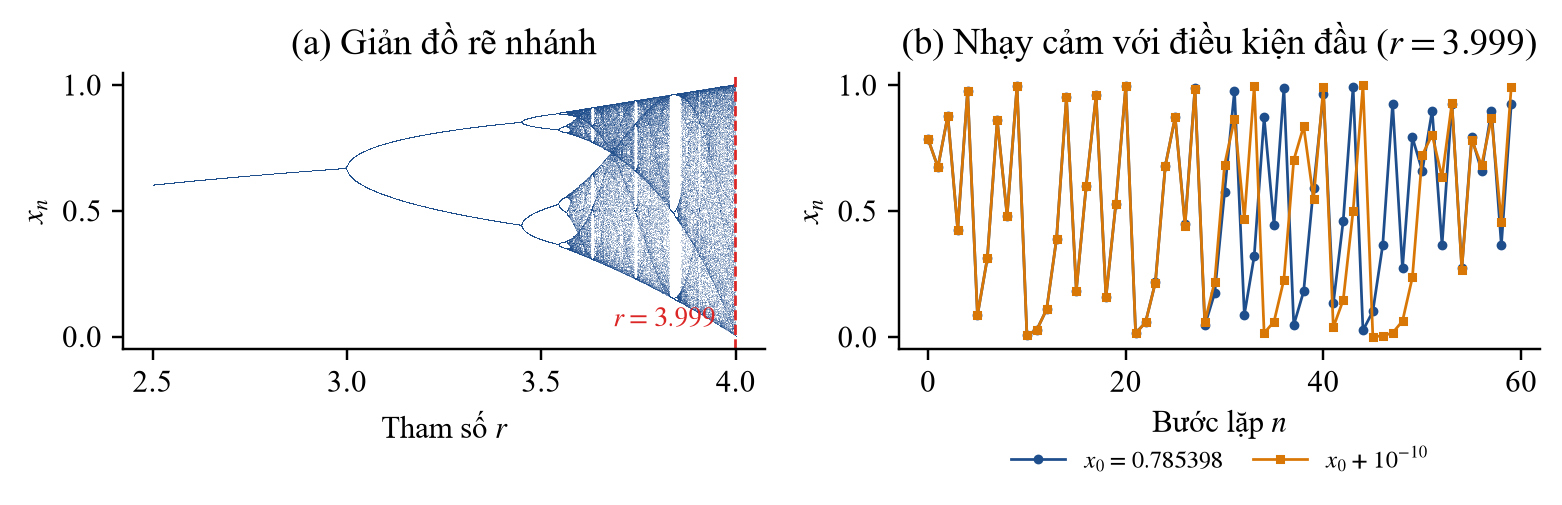
\includegraphics[width=\linewidth]{logistic_map}
\caption{Ánh xạ Logistic: (a) giản đồ rẽ nhánh theo $r$; (b) độ nhạy với điều kiện đầu}
\label{fig:logistic}
\end{figure}

Tuy vậy, cần lưu ý rằng ``hỗn loạn'' không đồng nghĩa với ``an toàn mật mã''. Alvarez và Li
\cite{alvarez2006} chỉ ra nhiều lược đồ mã hóa hỗn loạn bị phá vì không gian khóa nhỏ, phân bố
chuỗi không đều hoặc dùng lại dòng khóa. Đây là cơ sở để đánh giá lớp mã hóa hỗn loạn của bài
báo ở mục~\ref{sec:antoan-morong}.

\subsubsection{Toán tử XOR và mã dòng}

Phép XOR ($\xor$) có các tính chất giao hoán, kết hợp, $A \xor 0 = A$ và tự nghịch đảo
$A \xor A = 0$. Do đó nếu $C = P \xor K$ thì $P = C \xor K$, tức cùng một phép toán được dùng cho
cả mã hóa và giải mã. Khi dòng khóa $K$ thật sự ngẫu nhiên, dài bằng bản rõ và \emph{chỉ dùng một
lần}, ta có sổ mật mã dùng một lần (\tn{one-time pad}), an toàn tuyệt đối theo Shannon
\cite{shannon1949}. Ngược lại, nếu cùng một dòng khóa được dùng cho hai bản rõ $P_1, P_2$ thì:
\begin{equation}
  C_1 \xor C_2 = (P_1 \xor K) \xor (P_2 \xor K) = P_1 \xor P_2,
  \label{eq:twotime}
\end{equation}
nghĩa là dòng khóa bị triệt tiêu và cấu trúc của hai bản rõ lộ ra. Hơn nữa, chỉ cần biết một
cặp $(P_1, C_1)$ là kẻ tấn công khôi phục được $K = P_1 \xor C_1$ \cite{katz2020}.

\subsubsection{Giấu tin LSB đa bit}

Với điểm ảnh 8 bit có giá trị $c$, kỹ thuật \textbf{$k$-LSB} thay $k$ bit thấp nhất của $c$ bằng
một nhóm $k$ bit thông điệp có giá trị $m \in \{0, \dots, 2^k - 1\}$:
\begin{equation}
  s = c - (c \bmod 2^k) + m, \qquad |s - c| \le 2^k - 1.
  \label{eq:klsb}
\end{equation}
Mỗi kênh màu R, G, B được dùng như một ``điểm'' nhúng độc lập nên ảnh màu $H \times W$ có dung
lượng $3HWk$ bit. \hinh{fig:lsb-example} minh họa nhúng 1 bit và 3 bit vào một giá trị kênh màu.

\begin{figure}[H]
\centering
\begin{tikzpicture}[
  bit/.style={draw, minimum width=6mm, minimum height=6mm, font=\ttfamily\small, inner sep=0pt},
  hb/.style={bit, fill=orange!25}]
  \node[anchor=east] at (-0.2, 0) {$c = 154$:};
  \foreach \b [count=\i] in {1,0,0,1,1,0,1,0}{ \node[bit] at (\i*0.6, 0) {\b}; }
  \node[anchor=east] at (-0.2, -1) {1-LSB, $m=1$:};
  \foreach \b [count=\i] in {1,0,0,1,1,0,1}{ \node[bit] at (\i*0.6, -1) {\b}; }
  \node[hb] at (4.8, -1) {1};
  \node[anchor=west] at (5.4, -1) {$s = 155,\ |s-c| = 1$};
  \node[anchor=east] at (-0.2, -2) {3-LSB, $m=5$:};
  \foreach \b [count=\i] in {1,0,0,1,1}{ \node[bit] at (\i*0.6, -2) {\b}; }
  \foreach \b [count=\i] in {1,0,1}{ \node[hb] at (3.0+\i*0.6, -2) {\b}; }
  \node[anchor=west] at (5.4, -2) {$s = 157,\ |s-c| = 3 \le 7$};
\end{tikzpicture}
\caption{Ví dụ nhúng 1-LSB và 3-LSB vào một giá trị kênh màu (ô tô màu là bit thông điệp)}
\label{fig:lsb-example}
\end{figure}

Khi bit thông điệp là ngẫu nhiên đều và độc lập với ảnh phủ (đúng với bản mã tốt), $k$ bit thấp
của $c$ và $m$ đều phân bố đều trên $\{0,\dots,L-1\}$ với $L = 2^k$. Sai số bình phương kỳ vọng
tại mỗi kênh khi đó bằng:
\begin{equation}
  \mathbb{E}\bigl[(s-c)^2\bigr] = 2\,\mathrm{Var}(U_L) = \frac{L^2 - 1}{6}
  = \begin{cases} 0.5 & k = 1,\\ 2.5 & k = 2,\\ 10.5 & k = 3. \end{cases}
  \label{eq:lsb-mse}
\end{equation}
Công thức \pt{eq:lsb-mse} là chìa khóa để giải thích các con số MSE và PSNR trong bài báo:
nhúng 1-LSB lấp đầy toàn bộ ảnh cho $\mathrm{MSE} \approx 0.5$, tương ứng
$\mathrm{PSNR} = 10\log_{10}(255^2/0.5) \approx \SI{51.14}{dB}$.

\subsection{Tiêu chí đánh giá}
\label{sec:tieuchi}

Bài báo dùng ba nhóm tiêu chí: chất lượng thị giác của ảnh mang tin, độ an toàn thống kê của bản
mã và tốc độ thực thi.

\subsubsection{Sai số bình phương trung bình và PSNR}

Với ảnh phủ $I$ và ảnh mang tin $K$ kích thước $M \times N$ (mỗi điểm ảnh có $c$ kênh):
\begin{equation}
  \mathrm{MSE} = \frac{1}{MNc}\sum_{i,j,ch}\bigl[I(i,j,ch) - K(i,j,ch)\bigr]^2, \qquad
  \mathrm{PSNR} = 10\log_{10}\frac{255^2}{\mathrm{MSE}} \;(\mathrm{dB}).
  \label{eq:mse-psnr}
\end{equation}
MSE càng nhỏ và PSNR càng lớn thì ảnh mang tin càng giống ảnh phủ; PSNR trên khoảng
\SI{40}{dB} thường được coi là không phân biệt được bằng mắt thường. Bài báo ghi mẫu số của MSE
là $M \times N$; tuy nhiên để ra được $\mathrm{MSE} \approx 0.5$ như Bảng~2 của bài báo thì phải
chia cho toàn bộ $M \times N \times 3$ phần tử (giống hàm \code{immse} của MATLAB).

\subsubsection{Chỉ số tương đồng cấu trúc SSIM}

SSIM \cite{wang2004ssim} so sánh độ sáng, độ tương phản và cấu trúc cục bộ của hai ảnh $x, y$:
\begin{equation}
  \mathrm{SSIM}(x,y) = \frac{(2\mu_x\mu_y + C_1)(2\sigma_{xy} + C_2)}
                            {(\mu_x^2 + \mu_y^2 + C_1)(\sigma_x^2 + \sigma_y^2 + C_2)},
  \label{eq:ssim}
\end{equation}
trong đó $\mu$, $\sigma^2$, $\sigma_{xy}$ là trung bình, phương sai và hiệp phương sai tính trên cửa
sổ trượt; $C_1 = (0.01\cdot255)^2$, $C_2 = (0.03\cdot255)^2$. SSIM nằm trong $[-1, 1]$ và bằng 1
khi hai ảnh giống hệt nhau.

\subsubsection{Phân tích histogram}

Histogram biểu diễn tần suất xuất hiện của từng mức xám. Ảnh tự nhiên có histogram nhiều đỉnh,
không đều; một thuật toán mã hóa tốt phải cho histogram bản mã gần như \emph{phẳng}, nhờ đó chống
được tấn công thống kê. Ngược lại, histogram của ảnh mang tin phải gần như trùng với histogram ảnh
phủ để không để lại dấu vết.

\subsubsection{Phân tích vi sai: NPCR và UACI}

NPCR (\tn{Number of Pixels Change Rate}) đo tỷ lệ điểm ảnh khác nhau giữa hai ảnh $I_1, I_2$
kích thước $m\times n$; UACI (\tn{Unified Average Changing Intensity}) đo độ chênh cường độ trung
bình \cite{wu2011npcr}:
\begin{equation}
  \mathrm{NPCR} = \frac{1}{mn}\sum_{i,j} D(i,j)\times100\%, \quad
  D(i,j) = \begin{cases}0 & I_1(i,j) = I_2(i,j)\\ 1 & I_1(i,j) \neq I_2(i,j)\end{cases},
  \label{eq:npcr}
\end{equation}
\begin{equation}
  \mathrm{UACI} = \frac{1}{mn}\sum_{i,j}\frac{|I_1(i,j) - I_2(i,j)|}{255}\times100\%.
  \label{eq:uaci}
\end{equation}
Với hai ảnh ngẫu nhiên đều và độc lập, giá trị kỳ vọng là
$\mathrm{NPCR} = (1 - 2^{-8})\times100\% \approx 99.609\%$ và $\mathrm{UACI} \approx 33.464\%$
\cite{wu2011npcr}. Cần lưu ý: theo định nghĩa chuẩn của phân tích vi sai, $I_1$ và $I_2$ là
\emph{hai bản mã} của hai bản rõ chỉ khác nhau một điểm ảnh. Bài báo lại tính NPCR, UACI giữa
\emph{ảnh bí mật và bản mã của chính nó}; khác biệt này được phân tích ở
mục~\ref{sec:antoan-morong}.

\subsubsection{Entropy thông tin}

Entropy Shannon \cite{shannon1948} đo độ bất định trung bình của một điểm ảnh:
\begin{equation}
  H = -\sum_{i=0}^{L-1} p_i \log_2 p_i \quad (\text{bit}),
  \label{eq:entropy}
\end{equation}
với $L = 256$ mức xám và $p_i$ là xác suất xuất hiện mức $i$. Giá trị tối đa là 8 bit, đạt được
khi phân bố đều; bản mã tốt phải có entropy rất gần 8.

\subsubsection{Hệ số tương quan}

Hệ số tương quan Pearson giữa hai dãy giá trị $x, y$ độ dài $N$:
\begin{equation}
  r_{xy} = \frac{\sum_{i=1}^N (x_i - \bar x)(y_i - \bar y)}
                {\sqrt{\sum_{i=1}^N (x_i - \bar x)^2}\sqrt{\sum_{i=1}^N (y_i - \bar y)^2}}.
  \label{eq:corr}
\end{equation}
Bài báo dùng $r$ giữa ảnh bí mật và bản mã (kỳ vọng $r \approx 0$). Một cách dùng phổ biến khác
là tương quan giữa các cặp \emph{điểm ảnh kề nhau} theo chiều ngang, dọc, chéo: ảnh tự nhiên có
$r$ gần 1, bản mã tốt phải có $r$ gần 0.

\subsubsection{Thời gian mã hóa}

Thời gian mã hóa (\tn{EncTime}) đo chi phí tính toán của bước mã hóa ảnh bí mật; giá trị càng nhỏ
thì thuật toán càng phù hợp cho ứng dụng thời gian thực hoặc thiết bị hạn chế tài nguyên.

\subsection{Kỹ thuật áp dụng trong bài báo}

\subsubsection{Kiến trúc tổng thể}

Khung đề xuất gồm hai lớp nối tiếp (\hinh{fig:paper-arch}). Ở phía gửi, ảnh bí mật xám được
chuyển thành chuỗi byte và mã hóa thành ``ảnh mã hóa'' trông như nhiễu; sau đó bản mã được nhúng
vào các bit LSB của ảnh phủ màu để tạo ảnh mang tin. Ở phía nhận, các bit LSB được trích xuất để
dựng lại bản mã và giải mã bằng đúng khóa để thu lại ảnh bí mật.

\begin{figure}[H]
\centering
\resizebox{\linewidth}{!}{%
\begin{tikzpicture}[every node/.append style={font=\footnotesize}]
  \node[box] (si) {Ảnh bí mật\\(xám)};
  \node[pbox, right=8mm of si] (enc) {Mã hóa\\3DES / AES / Chaotic};
  \node[pbox, right=17mm of enc] (st) {Giấu tin\\LSB (1--3 bit)};
  \node[box, above=7mm of st] (cov) {Ảnh phủ\\RGB $256\times256$};
  \node[pbox, right=22mm of st] (dr) {Trích xuất\\và giải mã};
  \node[box, right=8mm of dr] (rs) {Ảnh bí mật\\khôi phục};
  \draw[arr] (si) -- (enc);
  \draw[arr] (enc) -- node[lbl, above] {bản mã} (st);
  \draw[arr] (cov) -- (st);
  \draw[arr] (st) -- node[lbl, above, pos=0.28] {ảnh stego} (dr);
  \draw[arr] (dr) -- (rs);
  \node[lbl, below=2mm of enc] {khóa $K$};
  \node[lbl, below=2mm of dr] {khóa $K$};
  \coordinate (mid) at ($(st.east)!0.6!(dr.west)$);
  \draw[dashed, gray] ($(mid)+(0,0.9)$) -- ($(mid)+(0,-0.8)$);
  \node[lbl, gray, anchor=south] at ($(mid)+(0,0.9)$) {kênh công khai};
\end{tikzpicture}}
\caption{Sơ đồ khối của hệ mật mã -- giấu tin kết hợp (vẽ lại theo Hình~1 của bài báo
\cite{raut2026hybrid})}
\label{fig:paper-arch}
\end{figure}

\subsubsection{Phương pháp 3DES-LSB}

\begin{enumerate}
  \item Chuyển ảnh bí mật thành chuỗi byte; mã hóa bằng 3DES khóa 192 bit (24 byte), IV 64 bit
        (8 byte), chế độ CBC, trình tự EDE.
  \item Xác định số bit LSB cần dùng trên mỗi kênh màu (1--3 bit) từ kích thước bản mã và số điểm
        ảnh của ảnh phủ.
  \item Chuyển bản mã thành chuỗi bit và nhúng vào các bit LSB của ảnh phủ RGB.
  \item Phía nhận trích các bit LSB, dựng lại bản mã, giải mã bằng cùng khóa và IV.
  \item Định hình lại (\tn{reshape}) dữ liệu giải mã về kích thước ban đầu của ảnh bí mật.
  \item Tính các độ đo chất lượng (MSE, PSNR, SSIM) và an toàn (NPCR, UACI, tương quan, entropy).
\end{enumerate}

\subsubsection{Phương pháp AES-LSB}

Quy trình hoàn toàn tương tự 3DES-LSB, chỉ khác lớp mã hóa: AES-128 với khóa 16 byte, IV 16 byte,
chế độ CBC. Kích thước khối 128 bit khiến bản mã được đệm thành bội số của 16 byte.

\subsubsection{Phương pháp Chaotic + PRNG Masking}

Lớp mã hóa thứ ba là một mã dòng gồm hai mặt nạ cùng độ dài $N$ với chuỗi byte ảnh bí mật $S$
(\hinh{fig:paper-chaotic}):
\begin{itemize}
  \item \textbf{Mặt nạ hỗn loạn}: sinh dãy $\{x_n\}$ theo \pt{eq:logistic} với $x_0 = 0.785398$,
        $r = 3.999$, rồi co giãn về khoảng $0$--$255$;
  \item \textbf{Mặt nạ ``ECC'' mô phỏng}: một dãy byte giả ngẫu nhiên sinh từ một hạt giống
        (\tn{seed}) cố định, được tác giả gọi là mô phỏng dòng khóa ECC.
\end{itemize}
Bản mã được tính bằng hai phép XOR liên tiếp, và giải mã chính là lặp lại đúng phép toán đó:
\begin{equation}
  \mathit{encBytes} = S \xor \mathit{chaosMask} \xor \mathit{eccMask}.
  \label{eq:chaotic}
\end{equation}
Nếu số bit cần nhúng vượt quá dung lượng 3-LSB, ảnh phủ được phóng to trước khi nhúng.

\begin{figure}[H]
\centering
\resizebox{0.92\linewidth}{!}{%
\begin{tikzpicture}[every node/.append style={font=\footnotesize}]
  \node[box] (s) at (0,0) {Ảnh bí mật\\dạng byte $S$};
  \node[xorn] (x1) at (3.6,0) {$\oplus$};
  \node[xorn] (x2) at (8.4,0) {$\oplus$};
  \node[box] (out) at (11.4,0) {Bản mã\\\textit{encBytes}};
  \node[pbox] (cm) at (3.6,2.1) {Sinh mặt nạ hỗn loạn\\Logistic $(x_0,\, r,\, N)$};
  \node[pbox] (em) at (8.4,2.1) {Sinh mặt nạ ``ECC'' (PRNG)\\seed cố định, độ dài $N$};
  \draw[arr] (s) -- (x1);
  \draw[arr] (cm) -- node[lbl, right] {\textit{chaosMask}} (x1);
  \draw[arr] (x1) -- (x2);
  \draw[arr] (em) -- node[lbl, right] {\textit{eccMask}} (x2);
  \draw[arr] (x2) -- (out);
\end{tikzpicture}}
\caption{Lớp mã hóa Chaotic + PRNG Masking (vẽ lại theo Hình~2 của bài báo \cite{raut2026hybrid})}
\label{fig:paper-chaotic}
\end{figure}

\subsubsection{So sánh ba phương pháp}

\bang{tab:paper-table1} tóm tắt các thông số kỹ thuật của ba phương pháp theo Bảng~1 của bài báo.

\begin{table}[H]
\centering
\caption{So sánh ba phương pháp trong bài báo (theo Bảng~1 của \cite{raut2026hybrid})}
\label{tab:paper-table1}
\small
\begin{tabularx}{\linewidth}{@{}P{2.6cm}LLL@{}}
\toprule
\thead{Tiêu chí} & \thead{3DES-LSB} & \thead{AES-LSB} & \thead{Chaotic-LSB}\\
\midrule
Thuật toán & 3DES 192 bit, CBC & AES 128 bit, CBC & Logistic + mặt nạ PRNG\\
Kích thước khối & 64 bit & 128 bit & Không có (mã dòng)\\
Khóa / tham số & Khóa 24 byte + IV 8 byte & Khóa 16 byte + IV 16 byte & $x_0 = 0.785398$, $r = 3.999$, mặt nạ ECC mô phỏng\\
Đệm & Bội số 8 byte & Bội số 16 byte & Không đệm\\
\bottomrule
\end{tabularx}
\end{table}

\subsubsection{Thực nghiệm và kết quả công bố}

Bài báo thực nghiệm trên bộ dữ liệu \textbf{Linnaeus 5} \cite{chaladze2017} gồm 8000 ảnh màu
$256\times256$ thuộc 5 lớp \code{berry}, \code{bird}, \code{dog}, \code{flower}, \code{other}
(mỗi lớp 1200 ảnh huấn luyện và 400 ảnh kiểm tra). Ảnh bí mật là ảnh xám ``coins'' có sẵn trong
MATLAB. Mỗi ảnh của Linnaeus 5 lần lượt làm ảnh phủ; các độ đo được tính trung bình trên toàn bộ
8000 ảnh và trình bày trong \bang{tab:paper-table2}.

\begin{table}[H]
\centering
\caption{Kết quả công bố trong Bảng~2 của bài báo (trung bình trên 8000 ảnh)}
\label{tab:paper-table2}
\small
\begin{tabular}{@{}lrrr@{}}
\toprule
\thead{Độ đo} & \thead{3DES} & \thead{AES} & \thead{Chaotic + PRNG}\\
\midrule
MSE                  & 0.499975 & 0.500006 & 0.499321\\
PSNR (dB)            & 51.15389 & 51.15373 & 51.14436\\
SSIM                 & 0.998495 & 0.998494 & 0.998099\\
EncTime (s)          & 0.003552 & 0.000601 & 3.62E-05\\
NPCR (\%)            & 99.59214 & 99.61924 & 99.63957\\
UACI (\%)            & 30.80843 & 30.81756 & 30.96067\\
Hệ số tương quan     & 0.00032  & $-0.00407$ & $-0.00984$\\
Entropy              & 7.047627 & 7.047762 & 6.952836\\
\bottomrule
\end{tabular}
\end{table}

Từ các kết quả trên, bài báo kết luận: chất lượng thị giác của ba phương pháp gần như như nhau
(PSNR $\approx$ \SI{51.15}{dB}, SSIM $\approx 0.998$); phương pháp hỗn loạn nhanh hơn AES khoảng 17
lần và nhanh hơn 3DES khoảng 98 lần, có NPCR/UACI nhỉnh hơn nhưng entropy thấp hơn (6.95 so với
khoảng 7.05); lựa chọn phương pháp tùy thuộc yêu cầu về tốc độ hay về tuân thủ chuẩn mật mã.

\subsection{Ưu nhược điểm của giải pháp đề xuất}

\subsubsection{Ưu điểm}

\begin{itemize}
  \item \textbf{Bảo vệ hai lớp}: lớp mã hóa bảo vệ nội dung, lớp giấu tin che giấu sự tồn tại của
        thông điệp; ngay cả khi bị trích xuất, dữ liệu vẫn vô nghĩa nếu không có khóa.
  \item \textbf{Chất lượng ảnh mang tin cao}: ở chế độ 1-LSB, PSNR đạt trên \SI{51}{dB}, sai khác
        hoàn toàn không nhận thấy bằng mắt thường.
  \item \textbf{Thiết kế mô-đun}: cùng một khung có thể thay lớp mã hóa (3DES, AES, hỗn loạn) mà
        không ảnh hưởng lớp giấu tin.
  \item \textbf{Thực nghiệm quy mô lớn}: đánh giá trên 8000 ảnh với nhiều độ đo, có so sánh định
        lượng giữa ba thuật toán.
\end{itemize}

\subsubsection{Nhược điểm và các điểm chưa rõ}

Trong quá trình đọc và tái hiện, em nhận thấy bài báo còn một số hạn chế về mặt an toàn và nhiều
chi tiết kỹ thuật không được công bố, khiến việc tái hiện chính xác gặp khó khăn:
\begin{itemize}
  \item \textbf{Thiếu chi tiết cài đặt}: không công bố kích thước ảnh bí mật, giá trị khóa/IV, cách
        lượng tử hóa dãy Logistic về byte, chuẩn đệm, thứ tự trải phẳng điểm ảnh, công thức phóng to
        ảnh phủ và cách bên nhận biết số bit LSB, kích thước ảnh, độ dài bản mã.
  \item \textbf{Mâu thuẫn nội tại}: nếu dùng ảnh ``coins'' $246\times300$ thì bắt buộc phải nhúng
        3-LSB và MSE phải khoảng 10.5 theo \pt{eq:lsb-mse}, trong khi Bảng~2 báo MSE $\approx 0.5$
        (đặc trưng của 1-LSB). Entropy $\approx 7.05$ cũng quá thấp so với một bản mã tốt
        ($\approx 8$), gợi ý rằng entropy được đo trên ảnh mang tin chứ không phải trên bản mã.
  \item \textbf{Lớp ``ECC'' chỉ là mô phỏng}: không có phép toán đường cong elliptic nào; mặt nạ thực
        chất là đầu ra của một bộ sinh số giả ngẫu nhiên với seed cố định.
  \item \textbf{Quản lý khóa yếu}: các tham số $x_0$, $r$ của lớp hỗn loạn được công bố công khai,
        trái với nguyên lý Kerckhoffs; dòng khóa không phụ thuộc vào ảnh nên bị dùng lại cho mọi ảnh.
  \item \textbf{Giấu tin không bền vững}: kỹ thuật LSB thay thế bị phá hủy hoàn toàn khi ảnh bị
        nén JPEG hoặc thêm nhiễu, và dễ bị phát hiện bởi phân tích thống kê. Bài báo không đánh giá
        các khía cạnh này.
  \item \textbf{Không có cơ chế toàn vẹn}: chế độ CBC không xác thực bản mã, nên một ảnh mang tin bị
        sửa đổi vẫn có thể được giải mã ra dữ liệu sai mà không có cảnh báo.
\end{itemize}

Các điểm chưa rõ nói trên được giải quyết bằng mười quyết định thiết kế trình bày ở
mục~\ref{sec:diemmu}. Các hạn chế về an toàn được kiểm chứng bằng thực nghiệm ở
mục~\ref{sec:antoan-morong}.

% =====================================================================
\chapter{Vận dụng kỹ thuật trong báo cáo môn học}
\label{chap:vandung}
% =====================================================================

Để kiểm chứng các kết luận của bài báo, em đã cài đặt lại toàn bộ khung lai mật mã -- giấu tin
bằng ngôn ngữ Python thay cho MATLAB R2024a mà các tác giả sử dụng. Sản phẩm gồm ba phần: một
thư viện lõi (mã hóa, giấu tin, đánh giá), các kịch bản dòng lệnh để tái hiện Hình~4--5 và
Bảng~2 của bài báo, và một ứng dụng desktop chạy ngoại tuyến để trình diễn trực quan. Chương này
trình bày kiến trúc, các quyết định thiết kế, cách cài đặt, giao diện, kiểm thử và kết quả thực
nghiệm, kèm theo một số phân tích an toàn mở rộng mà bài báo chưa thực hiện.

\section{Mục tiêu và phạm vi tái hiện}

Các mục tiêu cụ thể của phần vận dụng:
\begin{enumerate}
  \item Cài đặt đúng ba lớp mã hóa (3DES-CBC, AES-128-CBC, Chaotic + PRNG) và lớp giấu tin LSB
        đa bit theo mô tả của bài báo, bảo đảm khôi phục ảnh bí mật \emph{chính xác từng bit}
        ($\mathrm{MSE} = 0$).
  \item Làm rõ và xử lý nhất quán các chi tiết bài báo không công bố hoặc mô tả mâu thuẫn.
  \item Tái hiện Hình~4, Hình~5 (một cặp ảnh mẫu) và Bảng~2 (8000 ảnh Linnaeus 5) của bài báo,
        đối chiếu định lượng với số liệu gốc.
  \item Đánh giá thêm các khía cạnh an toàn mà bài báo chưa đề cập: độ nhạy khóa, phân tích vi
        sai đúng định nghĩa, tấn công biết bản rõ, khả năng chống chỉnh sửa và khả năng bị phát hiện.
  \item Xây dựng ứng dụng desktop trực quan, đóng gói thành tệp thực thi chạy độc lập trên
        Windows.
\end{enumerate}

\section{Kiến trúc và luồng xử lý hệ thống}

\subsection{Công nghệ sử dụng}

Hệ thống được viết bằng Python 3.12 và chỉ dùng các thư viện mã nguồn mở phổ biến
(\bang{tab:tech}). Toàn bộ tham số thuật toán được tập trung trong một tệp cấu hình YAML duy nhất
(\path{configs/default.yaml}), không có giá trị nào được viết cứng trong mã nguồn.

\begin{table}[H]
\centering
\caption{Công nghệ và thư viện sử dụng}
\label{tab:tech}
\small
\begin{tabularx}{\linewidth}{@{}P{3.4cm}P{1.9cm}L@{}}
\toprule
\thead{Thư viện} & \thead{Phiên bản} & \thead{Vai trò}\\
\midrule
Python & 3.12.8 & Ngôn ngữ cài đặt (môi trường ảo \code{.venv})\\
PyCryptodome \cite{pycryptodome} & 3.24.1 & Mã khối DES3, AES chế độ CBC; đệm PKCS\#7\\
NumPy \cite{harris2020numpy} & 2.2.6 & Biểu diễn ảnh, thao tác bit vectơ hóa, sinh số giả ngẫu nhiên PCG64\\
Numba \cite{lam2015numba} & 0.68.1 & Biên dịch JIT vòng lặp ánh xạ Logistic sang mã máy\\
OpenCV \cite{bradski2000} & 4.14.0 & Đọc/ghi ảnh, phóng to ảnh phủ (nội suy bicubic), nén JPEG thử nghiệm\\
scikit-image \cite{vanderwalt2014} & 0.26.0 & SSIM cửa sổ Gauss; ảnh mẫu \code{coins}\\
SciPy, pandas & 1.18.1, 2.3.3 & Thống kê, kiểm định $\chi^2$; tổng hợp kết quả benchmark ra CSV\\
Matplotlib & 3.11.2 & Vẽ histogram và biểu đồ (giao diện OOP, không dùng \code{pyplot} trong GUI)\\
Tkinter/ttk, Pillow & 8.6, 13.0.0 & Giao diện desktop; hiển thị ảnh\\
pytest & 8.4.2 & Kiểm thử tự động (347 ca kiểm thử)\\
PyInstaller & 6.22.3 & Đóng gói ứng dụng thành tệp \code{.exe}\\
\bottomrule
\end{tabularx}
\end{table}

\subsection{Kiến trúc phân lớp}

Mã nguồn được tổ chức thành các gói độc lập theo trách nhiệm (\hinh{fig:architecture}). Tầng mã
hóa áp dụng \textbf{mẫu thiết kế Strategy}: lớp trừu tượng \code{BaseCipher} quy định giao diện
chung \code{encrypt(bytes) -> bytes} và \code{decrypt(bytes) -> bytes}, ba lớp con
\code{DES3Cipher}, \code{AESCipher}, \code{ChaoticCipher} cài đặt cụ thể, và hàm
\code{create\_cipher} khởi tạo thuật toán theo tên. Nhờ đó tầng giấu tin, tầng đánh giá và giao
diện chỉ phụ thuộc vào giao diện chung; việc thêm một thuật toán mới không phải sửa các tầng khác.

\begin{figure}[H]
\centering
\begin{adjustbox}{max width=\linewidth}
\begin{tikzpicture}[
  layer/.style={draw, rounded corners=3pt, fill=codebg, inner sep=4pt},
  mod/.style={box, text width=34mm, minimum height=11mm, font=\footnotesize},
  core/.style={box, text width=42mm, minimum height=16mm, font=\footnotesize},
  wide/.style={box, text width=144mm, minimum height=8mm, font=\footnotesize}]
  % tầng trình diễn: GUI và kịch bản dòng lệnh
  \node[mod, fill=tblhead] (app) {\code{app.py}\\GUI Tkinter (4 tab)};
  \node[mod, fill=tblhead, right=3.5mm of app]  (ctrl) {\code{ui/controller.py}\\nghiệp vụ của GUI};
  \node[mod, fill=tblhead, right=3.5mm of ctrl] (cli1) {\code{run\_single.py}\\Hình 4--5};
  \node[mod, fill=tblhead, right=3.5mm of cli1] (cli2) {\code{run\_benchmark.py}\\Bảng 2, CSV};
  % pipeline
  \node[wide, below=8mm of $(ctrl.south)!0.5!(cli1.south)$] (pipe)
      {\code{pipeline.py}: \code{hide()}, \code{reveal()}, \code{run\_pipeline()} --- mã hóa (đo thời gian)
       $\rightarrow$ nhúng $\rightarrow$ trích $\rightarrow$ giải mã $\rightarrow$ tính độ đo};
  % lõi
  \node[core, below=8mm of pipe] (stego) {\code{stego/lsb.py}\\header 16 byte\\nhúng/trích $k$-LSB};
  \node[core, left=4mm of stego] (crypto) {\code{crypto/}\\\code{BaseCipher} (Strategy)\\DES3, AES, Chaotic};
  \node[core, right=4mm of stego] (metrics) {\code{metrics/}\\\code{visual.py}, \code{security.py}\\MSE, PSNR, NPCR, \ldots};
  \node[wide, fill=white, below=8mm of stego] (cfg)
      {\code{config.py} + \code{default.yaml}: $x_0$, $r$, seed khóa, độ dài khóa/IV, kích thước ảnh phủ, số LSB tối đa};
  \begin{scope}[on background layer]
    \node[layer, fit=(app)(cli2)] {};
    \node[layer, fit=(crypto)(metrics)] {};
  \end{scope}
  \foreach \n in {app, ctrl, cli1, cli2}{ \draw[arr] (\n.south) -- (\n.south |- pipe.north); }
  \foreach \n in {crypto, stego, metrics}{
    \draw[arr] (\n.north |- pipe.south) -- (\n.north);
    \draw[arr, dashed] (\n.south |- cfg.north) -- (\n.south); }
\end{tikzpicture}
\end{adjustbox}
\caption{Kiến trúc phân lớp của hệ thống tái hiện}
\label{fig:architecture}
\end{figure}

\subsection{Luồng xử lý phía gửi và phía nhận}

\hinh{fig:flow} mô tả luồng dữ liệu hoàn chỉnh. Điểm khác biệt quan trọng so với bài báo là phía
nhận \textbf{chỉ cần ảnh mang tin và khóa}: mọi siêu dữ liệu cần thiết (số bit LSB, kích thước ảnh
bí mật, độ dài bản mã) được đọc từ một header 16 byte nhúng sẵn trong ảnh.

\begin{figure}[H]
\centering
\begin{tikzpicture}[node distance=5mm and 7mm, every node/.style={font=\footnotesize}]
  \node[box] (s) {Ảnh bí mật\\$H_s\times W_s$, uint8};
  \node[pbox, right=of s] (b) {\code{tobytes()}\\(thứ tự hàng)};
  \node[pbox, right=of b] (e) {\code{cipher.encrypt}\\(đo EncTime)};
  \node[pbox, right=of e] (h) {Header 16 B\\+ bản mã};
  \node[pbox, right=of h] (em) {\code{lsb.embed}\\$k$-LSB};
  \node[box, above=of em] (c) {Ảnh phủ RGB\\$256\times256$};
  \node[box, below=8mm of em] (st) {Ảnh stego\\(.png)};
  \node[pbox, left=of st] (ex) {\code{lsb.extract}\\đọc header};
  \node[pbox, left=of ex] (d) {\code{cipher.decrypt}\\gỡ đệm};
  \node[pbox, left=of d] (r) {reshape\\$(H_s, W_s)$};
  \node[box, left=of r] (rec) {Ảnh khôi phục\\MSE $=0$};
  \draw[arr] (s) -- (b); \draw[arr] (b) -- (e); \draw[arr] (e) -- (h); \draw[arr] (h) -- (em);
  \draw[arr] (c) -- (em); \draw[arr] (em) -- (st); \draw[arr] (st) -- (ex);
  \draw[arr] (ex) -- (d); \draw[arr] (d) -- (r); \draw[arr] (r) -- (rec);
  \node[lbl, above=1mm of b, xshift=8mm] {\textbf{Phía gửi}};
  \node[lbl, below=1mm of d, xshift=8mm] {\textbf{Phía nhận}};
\end{tikzpicture}
\caption{Luồng xử lý gửi -- nhận của hệ thống}
\label{fig:flow}
\end{figure}

\subsection{Cấu trúc mã nguồn}

\begin{lstlisting}[style=plain, caption={Cấu trúc thư mục mã nguồn}, label={lst:tree}]
SOURCES/
|-- app.py                      # diem vao ung dung desktop
|-- configs/default.yaml        # nguon tham so duy nhat
|-- src/
|   |-- config.py               # doc YAML, chuan hoa duong dan
|   |-- pipeline.py             # hide / reveal / run_pipeline
|   |-- crypto/  base.py, des3_cipher.py, aes_cipher.py, chaotic_cipher.py
|   |-- stego/   lsb.py         # header 16 byte + nhung/trich k-LSB
|   |-- metrics/ visual.py, security.py
|   `-- ui/      app_window.py, controller.py, worker.py, plots.py, tabs/...
|-- scripts/     run_single.py, run_benchmark.py
|-- tests/       test_crypto.py, test_lsb.py, test_metrics.py,
|                test_pipeline.py, test_ui_controller.py
|-- packaging/ct204_app.spec    # cau hinh PyInstaller
`-- results/     benchmark_results.csv, benchmark_summary_table2.csv, single/
\end{lstlisting}

\section{Giải quyết các điểm mù kỹ thuật của bài báo}
\label{sec:diemmu}

Bài báo không công bố mã nguồn và bỏ ngỏ nhiều chi tiết. Em đã liệt kê mười ``điểm mù''
(ký hiệu BM-01 đến BM-10). Với mỗi điểm mù, em so sánh các phương án và chọn một phương án duy
nhất có lý do rõ ràng (\bang{tab:bm}). Mục này trình bày chi tiết ba quyết định ảnh hưởng nhiều
nhất đến việc đối chiếu kết quả.

{\small
\begin{longtable}{@{}P{1.3cm}P{5.6cm}P{8.1cm}@{}}
\caption{Mười điểm mù kỹ thuật và quyết định thiết kế đã chọn}
\label{tab:bm}\\
\toprule
\thead{Mã} & \thead{Điểm mù trong bài báo} & \thead{Quyết định thiết kế}\\
\midrule
\endfirsthead
\toprule
\thead{Mã} & \thead{Điểm mù trong bài báo} & \thead{Quyết định thiết kế}\\
\midrule
\endhead
\bottomrule
\endfoot
BM-01 & Không công bố kích thước ảnh ``coins''; mâu thuẫn giữa Hình~5 (3-LSB) và MSE $\approx 0.5$ ở Bảng~2 (1-LSB)
      & Ảnh mẫu chuẩn hóa về $246\times300$ (đúng \code{coins.png} của MATLAB) để tái hiện Hình~4--5; hỗ trợ tham số \code{--secret-size 156 156} để tái hiện Bảng~2 ở chế độ 1-LSB\\
BM-02 & Thứ tự trải phẳng byte (MATLAB theo cột, NumPy theo hàng)
      & Thống nhất thứ tự hàng (C-contiguous), kênh màu xen kẽ RGB $(H, W, 3)$ ở mọi bước\\
BM-03 & Không công bố khóa, IV, seed; không rõ dùng một khóa hay khóa riêng cho mỗi ảnh
      & Dẫn xuất tất định có phân tách miền: $\mathrm{SHA\text{-}256}(\text{seed}:\text{nhãn})$ làm hạt giống PRNG; mặc định khóa cố định, có tùy chọn \code{--vary-key-per-image}\\
BM-04 & Không nêu cách đưa $x_n \in (0,1)$ về byte; ``ECC'' không có đường cong elliptic
      & $\mathit{chaosMask}[n] = \min(\lfloor 256\,x_{n+1} \rfloor, 255)$ lấy từ $x_1$; mặt nạ ECC $=$ PCG64(\code{ecc\_seed}) sinh byte đều\\
BM-05 & Không nêu chuẩn đệm; bản mã sau đệm dài hơn $H_s W_s$ nên không reshape được
      & Đệm PKCS\#7, nhúng \emph{toàn bộ} bản mã; chỉ cắt $H_s W_s$ byte đầu khi hiển thị ảnh mã hóa và tính NPCR/UACI\\
BM-06 & Không có cơ chế truyền siêu dữ liệu sang phía nhận
      & Header nhị phân 16 byte (magic \code{HCST}, phiên bản, $k$, $H_s$, $W_s$, độ dài bản mã, CRC-16) nhúng ở 1-LSB của 128 giá trị kênh đầu tiên\\
BM-07 & Không nêu công thức phóng to ảnh phủ và ảnh đối chiếu khi tính MSE
      & Tăng $k$ từ 1 đến 3 trước; nếu vẫn thiếu thì phóng to đẳng hướng tối thiểu bằng nội suy bicubic; MSE tính giữa ảnh phủ \emph{đã dùng} và ảnh stego\\
BM-08 & Mâu thuẫn đối tượng đo entropy, NPCR, UACI, tương quan (bản mã hay ảnh stego)
      & Tính song song hai nhóm độ đo: \code{*\_enc} (ảnh bí mật -- bản mã) và \code{*\_stego} (ảnh phủ -- ảnh stego)\\
BM-09 & Mẫu số MSE ghi $M\times N$ cho ảnh màu; không nêu cửa sổ SSIM; hai cách hiểu về tương quan
      & MSE chia cho $H\times W\times3$; SSIM cửa sổ Gauss $11\times11$, $\sigma = 1.5$ (chuẩn Wang 2004, giống MATLAB); cài cả tương quan chéo và tương quan điểm ảnh kề\\
BM-10 & Cách vẽ histogram ảnh màu; phạm vi đo EncTime của Chaotic
      & Histogram 256 mức gộp phẳng cả 3 kênh (giống \code{img(:)} của MATLAB); Chaotic mặc định sinh lại mặt nạ mỗi lần, có chế độ ``cache mặt nạ'' để đo riêng phép XOR\\
\end{longtable}}

\paragraph{BM-01 -- Nghịch lý dung lượng 1-LSB và 3-LSB.}
Histogram bản mã ở Hình~5 của bài báo cao đều khoảng 288 điểm ảnh mỗi mức, tức tổng
$288.28 \times 256 \approx \num{73800}$ byte $= 246\times300$. Điều này chứng tỏ tác giả dùng
\code{coins.png} của MATLAB. Bản mã AES của ảnh này dài \num{73808} byte, vượt dung lượng 3-LSB của
ảnh $256\times256$ là $(3\cdot256^2 - 128)\cdot 3 / 8 = \num{73680}$ byte, nên bắt buộc phải nhúng
3-LSB và phóng to ảnh phủ. Theo \pt{eq:lsb-mse}, MSE khi đó phải xấp xỉ 10.5 chứ không thể là 0.5.
Ngược lại, $\mathrm{MSE} \approx 0.50$ và PSNR $\approx \SI{51.15}{dB}$ ở Bảng~2 là ``hằng số toán
học'' của phép nhúng 1-LSB gần lấp đầy ảnh, tương ứng tải tin khoảng \num{24500} byte, tức ảnh
khoảng $156\times156$. Vì vậy hệ thống hỗ trợ cả hai cấu hình: $246\times300$ để tái hiện
Hình~4--5 và $156\times156$ (\num{24336} byte, lấp $99.09\%$ dung lượng 1-LSB) để tái hiện Bảng~2.

\paragraph{BM-06 -- Header tự mô tả cho phép trích xuất ``mù''.}
Bài báo không cho biết phía nhận làm sao biết được số bit LSB, kích thước ảnh và độ dài bản mã.
Truyền các giá trị này qua kênh phụ thì không thực tế. Còn dùng chuỗi phân cách thì không an
toàn, vì bản mã là dữ liệu ngẫu nhiên nên có thể trùng chuỗi phân cách. Em thiết kế một header
nhị phân cố định 16 byte, luôn nhúng ở 1-LSB nên đọc được trước khi biết $k$. Chi tiết được trình
bày ở mục~\ref{sec:header}.

\paragraph{BM-08 -- Hai nhóm độ đo an toàn.}
Mục 4.4 của bài báo định nghĩa NPCR, UACI, entropy, tương quan giữa ảnh bí mật và bản mã, nhưng
bước 9 của thuật toán AES-LSB lại ghi tính các độ đo này ``cho mỗi ảnh stego''. Kiểm tra số liệu
cho thấy NPCR $\approx 99.6\%$ và tương quan $\approx 0$ chỉ có thể đến từ bản mã, trong khi
entropy $\approx 7.05$ lại giống entropy của một ảnh màu tự nhiên. Vì vậy hệ thống tính và xuất
\emph{cả hai nhóm}, để kết quả ở mục~\ref{sec:ketqua-antoan} có thể giải thích trọn vẹn Bảng~2.

\section{Cài đặt các thành phần chính}
\label{sec:caidat}

\subsection{Sinh khóa tất định có phân tách miền}

Để kết quả tái lập được giữa các lần chạy mà không phải lưu khóa vào ảnh, khóa và IV được dẫn xuất
tất định từ hạt giống \code{key\_seed = 2025} trong tệp cấu hình (\doanma{lst:derive}). Mỗi vai trò
dùng một nhãn riêng (\code{"aes:key"}, \code{"aes:iv"}, \code{"3des:key:0"}, \ldots). Đi qua
SHA-256 bảo đảm các khóa độc lập thống kê với nhau. Nếu khởi tạo PRNG trực tiếp bằng cùng một seed
thì 16 byte đầu của khóa 3DES sẽ trùng khóa AES. Với 3DES, nếu khóa dẫn xuất bị suy biến
($K_1 = K_2$ hoặc $K_2 = K_3$, khiến 3DES thoái hóa thành DES đơn), hệ thống thử nhãn kế tiếp
\code{"3des:key:1"}, \ldots{} cho đến khi được khóa hợp lệ.

\begin{lstlisting}[caption={Hàm dẫn xuất byte tất định có phân tách miền (\code{crypto/base.py})}, label={lst:derive}]
def derive_bytes(seed: int, length: int, label: str) -> bytes:
    digest = hashlib.sha256(f"{seed}:{label}".encode("utf-8")).digest()
    rng = np.random.default_rng(int.from_bytes(digest, "big"))
    return rng.integers(0, 256, size=length, dtype=np.uint8).tobytes()
\end{lstlisting}

Lưu ý rằng cơ chế này phục vụ \emph{tái lập thực nghiệm}, không phải cơ chế quản lý khóa an toàn:
ai biết seed trong tệp cấu hình đều dựng lại được khóa. Ứng dụng desktop vì thế bổ sung chế độ
``mật khẩu tùy chỉnh'', trong đó khóa của cả ba thuật toán được dẫn xuất từ
$\mathrm{SHA\text{-}256}(\code{"ct204-ui:"}\,\|\,\text{thuật toán}\,\|\,\text{mật khẩu})$.

\subsection{Mã hóa 3DES và AES ở chế độ CBC}

Hai lớp \code{DES3Cipher} và \code{AESCipher} có cấu trúc giống nhau (\doanma{lst:des3}): kiểm tra
độ dài khóa/IV ngay khi khởi tạo, tạo \emph{mới} đối tượng CBC cho mỗi lần gọi vì đối tượng CBC của
PyCryptodome có trạng thái và chỉ dùng được một lần, đệm PKCS\#7 khi mã hóa, và kiểm tra độ dài bản
mã là bội số của kích thước khối trước khi giải mã.

\begin{lstlisting}[caption={Lớp mã hóa 3DES-CBC (\code{crypto/des3\_cipher.py}, rút gọn)}, label={lst:des3}]
class DES3Cipher(BaseCipher):
    def __init__(self, key: bytes, iv: bytes) -> None:
        # raises ValueError for degenerate keys (K1 == K2 or K2 == K3)
        adjusted = DES3.adjust_key_parity(bytes(key))
        DES3.new(adjusted, DES3.MODE_CBC, iv=bytes(iv))
        self._key, self._iv = adjusted, bytes(iv)

    def _new(self):  # fresh CBC object per call: CBC objects are single-use
        return DES3.new(self._key, DES3.MODE_CBC, iv=self._iv)

    def encrypt(self, plaintext: bytes) -> bytes:
        return self._new().encrypt(pad(plaintext, 8, style="pkcs7"))

    def decrypt(self, ciphertext: bytes) -> bytes:
        if len(ciphertext) == 0 or len(ciphertext) % 8 != 0:
            raise ValueError("ciphertext length must be a positive multiple of 8")
        return unpad(self._new().decrypt(ciphertext), 8, style="pkcs7")
\end{lstlisting}

\subsection{Mã hóa hỗn loạn Chaotic + PRNG}

Vòng lặp ánh xạ Logistic có tính tuần tự ($x_{n+1}$ phụ thuộc $x_n$) nên không thể vectơ hóa bằng
NumPy. Em dùng Numba \cite{lam2015numba} để biên dịch vòng lặp sang mã máy (\doanma{lst:chaotic}).
Quy tắc lượng tử hóa $\lfloor 256\,x \rfloor$ chia đều khoảng $[0,1)$ thành đúng 256 khoảng con.
Cách \code{uint8(255*x)} của MATLAB (làm tròn) thì làm hai mức biên 0 và 255 chỉ rộng bằng một nửa
các mức khác. Để thời gian biên dịch JIT không bị tính vào EncTime, hàm \code{warmup()} chạy thử
hàm đã biên dịch trên 16 byte trước khi đo.

\begin{lstlisting}[caption={Sinh mặt nạ hỗn loạn và mã hóa XOR (\code{crypto/chaotic\_cipher.py}, rút gọn)}, label={lst:chaotic}]
@numba.njit(cache=True)
def logistic_mask(x0: float, r: float, n: int) -> np.ndarray:
    out = np.empty(n, dtype=np.uint8)
    x = x0
    for i in range(n):
        x = r * x * (1.0 - x)                  # logistic map, starts at x_1
        v = int(np.floor(x * 256.0))
        out[i] = 0 if v < 0 else (255 if v > 255 else v)
    return out

def ecc_mask(ecc_seed: int, n: int) -> np.ndarray:  # "simulated ECC" = seeded PRNG
    return np.random.default_rng(ecc_seed).integers(0, 256, size=n, dtype=np.uint8)

class ChaoticCipher(BaseCipher):
    def _xor(self, data: bytes) -> bytes:
        buf = np.frombuffer(data, dtype=np.uint8)
        mask = logistic_mask(self._x0, self._r, buf.size) ^ ecc_mask(self._ecc_seed, buf.size)
        return (buf ^ mask).tobytes()
    encrypt = decrypt = _xor                     # XOR is its own inverse
\end{lstlisting}

\subsection{Giao thức header 16 byte}
\label{sec:header}

Header được đóng gói bằng mô-đun \code{struct} của Python theo định dạng big-endian
\code{">4sBBHHIH"} (\hinh{fig:header}). Trường CRC-16 bằng 16 bit thấp của CRC-32 tính trên 14 byte đầu. Khi trích
xuất, hệ thống lần lượt kiểm tra magic, CRC, phiên bản, $k$, kích thước ảnh và việc bản mã có vượt
quá dung lượng ảnh hay không. Bất kỳ sai lệch nào cũng dừng quá trình với thông báo lỗi rõ ràng thay
vì giải mã ra dữ liệu rác. Header chỉ chiếm 128 bit, khoảng $0.065\%$ số giá trị kênh của ảnh
$256\times256$.

\begin{figure}[H]
\centering
\begin{bytefield}[bitwidth=0.9cm, bitheight=0.9cm]{16}
  \bitheader{0-15}\\
  \bitbox{4}{\small magic \code{"HCST"}} &
  \bitbox{1}{\scriptsize ver} &
  \bitbox{1}{\small $k$} &
  \bitbox{2}{\small $H_s$} &
  \bitbox{2}{\small $W_s$} &
  \bitbox{4}{\small \code{ciphertext\_len}} &
  \bitbox{2}{\small CRC-16}
\end{bytefield}

\vspace{4mm}
\begin{tikzpicture}[x=0.96cm, y=1cm]
  \draw[fill=orange!25] (0,0) rectangle (1.6,0.7) node[midway, font=\scriptsize, align=center] {Header\\1-LSB};
  \draw[fill=tblhead] (1.6,0) rectangle (11.0,0.7) node[midway, font=\scriptsize] {Bản mã: $8\cdot\mathit{len}$ bit, mỗi giá trị kênh chứa $k$ bit};
  \draw[fill=white] (11.0,0) rectangle (14.4,0.7) node[midway, font=\scriptsize] {Không thay đổi};
  \node[font=\scriptsize, below] at (0,0) {0};
  \node[font=\scriptsize, below] at (1.6,0) {128};
  \node[font=\scriptsize, below] at (11.0,0) {$128 + \lceil 8\,\mathit{len}/k \rceil$};
  \node[font=\scriptsize, below] at (14.4,0) {$3HW$};
  \node[font=\scriptsize, anchor=east] at (-0.1,0.35) {\code{flat}};
\end{tikzpicture}
\caption{Cấu trúc header 16 byte (trên) và bố cục nhúng trên mảng kênh màu trải phẳng (dưới)}
\label{fig:header}
\end{figure}

\subsection{Nhúng và trích xuất LSB vectơ hóa}

Ảnh phủ $(H, W, 3)$ được trải phẳng thành mảng \code{flat} gồm $M = 3HW$ giá trị kênh. Số bit LSB
$k$ được chọn là giá trị nhỏ nhất trong $\{1, 2, 3\}$ thỏa $8\cdot\mathit{len} \le (M - 128)\,k$.
Nếu ngay cả $k = 3$ cũng không đủ, ảnh phủ được phóng to đẳng hướng với hệ số tối thiểu
\begin{equation}
  s = \sqrt{\frac{\lceil 8\,\mathit{len}/3 \rceil + 128}{3HW}}, \qquad
  H' = \lceil sH \rceil,\; W' = \lceil sW \rceil,
  \label{eq:scaleup}
\end{equation}
bằng nội suy bicubic. Ví dụ, ảnh ``coins'' $246\times300$ chỉ làm ảnh phủ tăng từ $256\times256$
lên $257\times257$.

Toàn bộ thao tác bit được vectơ hóa hoàn toàn bằng NumPy, không có vòng lặp Python trên từng điểm
ảnh (\doanma{lst:lsb}). Chuỗi bit được chia thành nhóm $k$ bit, mỗi nhóm được đổi thành một ``ký
hiệu'' $m \in [0, 2^k)$ bằng tích vô hướng với vectơ trọng số $(2^{k-1}, \dots, 2, 1)$, rồi ghi vào
$k$ bit thấp bằng phép AND/OR theo \pt{eq:klsb}.

\begin{lstlisting}[caption={Ghi và đọc $k$ bit thấp theo kiểu vectơ hóa (\code{stego/lsb.py})}, label={lst:lsb}]
def _write_lsb(values: np.ndarray, bits: np.ndarray, k: int) -> np.ndarray:
    n = values.size
    groups = np.zeros(n * k, dtype=np.uint8)
    groups[: bits.size] = bits                       # zero-pad the last group
    weights = (1 << np.arange(k - 1, -1, -1)).astype(np.uint8)
    symbols = (groups.reshape(n, k) * weights).sum(axis=1, dtype=np.uint16).astype(np.uint8)
    keep = np.uint8(0xFF ^ ((1 << k) - 1))           # e.g. k=3 -> 0b11111000
    return (values & keep) | symbols

def _read_lsb(values: np.ndarray, k: int, n_bits: int) -> np.ndarray:
    shifts = np.arange(k - 1, -1, -1, dtype=np.uint8)
    bits = (values[:, None] >> shifts) & np.uint8(1)
    return bits.reshape(-1)[:n_bits]
\end{lstlisting}

\subsection{Đo lường và đánh giá}

Mô-đun \code{metrics} cài đặt các công thức ở mục~\ref{sec:tieuchi} dưới dạng hàm thuần, nhận hai
ảnh \code{uint8} bất kỳ (2D hoặc 3D), nhờ đó cùng một hàm dùng được cho cả cặp (ảnh bí mật, bản mã)
lẫn cặp (ảnh phủ, ảnh stego). Mọi phép trừ được thực hiện trên \code{float64} để tránh tràn số
\code{uint8}. Thời gian mã hóa được đo bằng \code{time.perf\_counter()} bao quanh \emph{duy nhất}
lời gọi \code{cipher.encrypt}, sau khi đã khởi động (\doanma{lst:enctime}).

\begin{lstlisting}[caption={Đo thời gian mã hóa (\code{metrics/security.py}, rút gọn)}, label={lst:enctime}]
def measure_enc_time(cipher, plaintext: bytes, *, warmup: bool = True):
    if warmup:
        cipher.warmup()                          # compile Numba JIT outside the timer
        if getattr(cipher, "cache_mask", False):
            cipher.combined_mask(len(plaintext)) # cached mode: time only the XOR
    t0 = time.perf_counter()
    ciphertext = cipher.encrypt(plaintext)
    return ciphertext, time.perf_counter() - t0
\end{lstlisting}

\section{Giao diện ứng dụng desktop}

\subsection{Tổng quan}

Ngoài các kịch bản dòng lệnh, em xây dựng một ứng dụng desktop bằng Tkinter/ttk để trình diễn
toàn bộ khung trực quan và chạy hoàn toàn ngoại tuyến. Ứng dụng gồm bốn tab tương ứng bốn kịch bản
sử dụng. Các tác vụ nặng như mã hóa, nhúng hay chạy so sánh được đưa sang luồng nền; kết quả trả về
luồng giao diện qua hàng đợi \code{queue.Queue} và cơ chế \code{after()} của Tk, nên giao diện
không bị treo. Biểu đồ được vẽ bằng giao diện hướng đối tượng của Matplotlib nhúng vào Tk. Ứng dụng
gọi lại đúng các hàm lõi của thư viện, không sửa bất kỳ tệp lõi nào, nên kết quả trên giao diện
trùng khớp bit với kết quả của kịch bản dòng lệnh.

\subsection{Tab 1 -- Mã hóa và giấu tin}

Người dùng chọn ảnh phủ, ảnh bí mật, chế độ kích thước ảnh bí mật (giữ nguyên $246\times300$ theo
Hình~4--5, $156\times156$ theo Bảng~2, hoặc tùy chọn), thuật toán và chế độ khóa (khóa mặc định của
bài báo hoặc mật khẩu tùy chỉnh). Kết quả hiển thị bốn ảnh (ảnh phủ thực dùng, ảnh bí mật, bản mã,
ảnh stego hoặc bản đồ sai khác khuếch đại), các chỉ số chính, bảng hai nhóm độ đo an toàn và ba
histogram (\hinh{fig:ui-tab1}).

\begin{figure}[H]
\centering
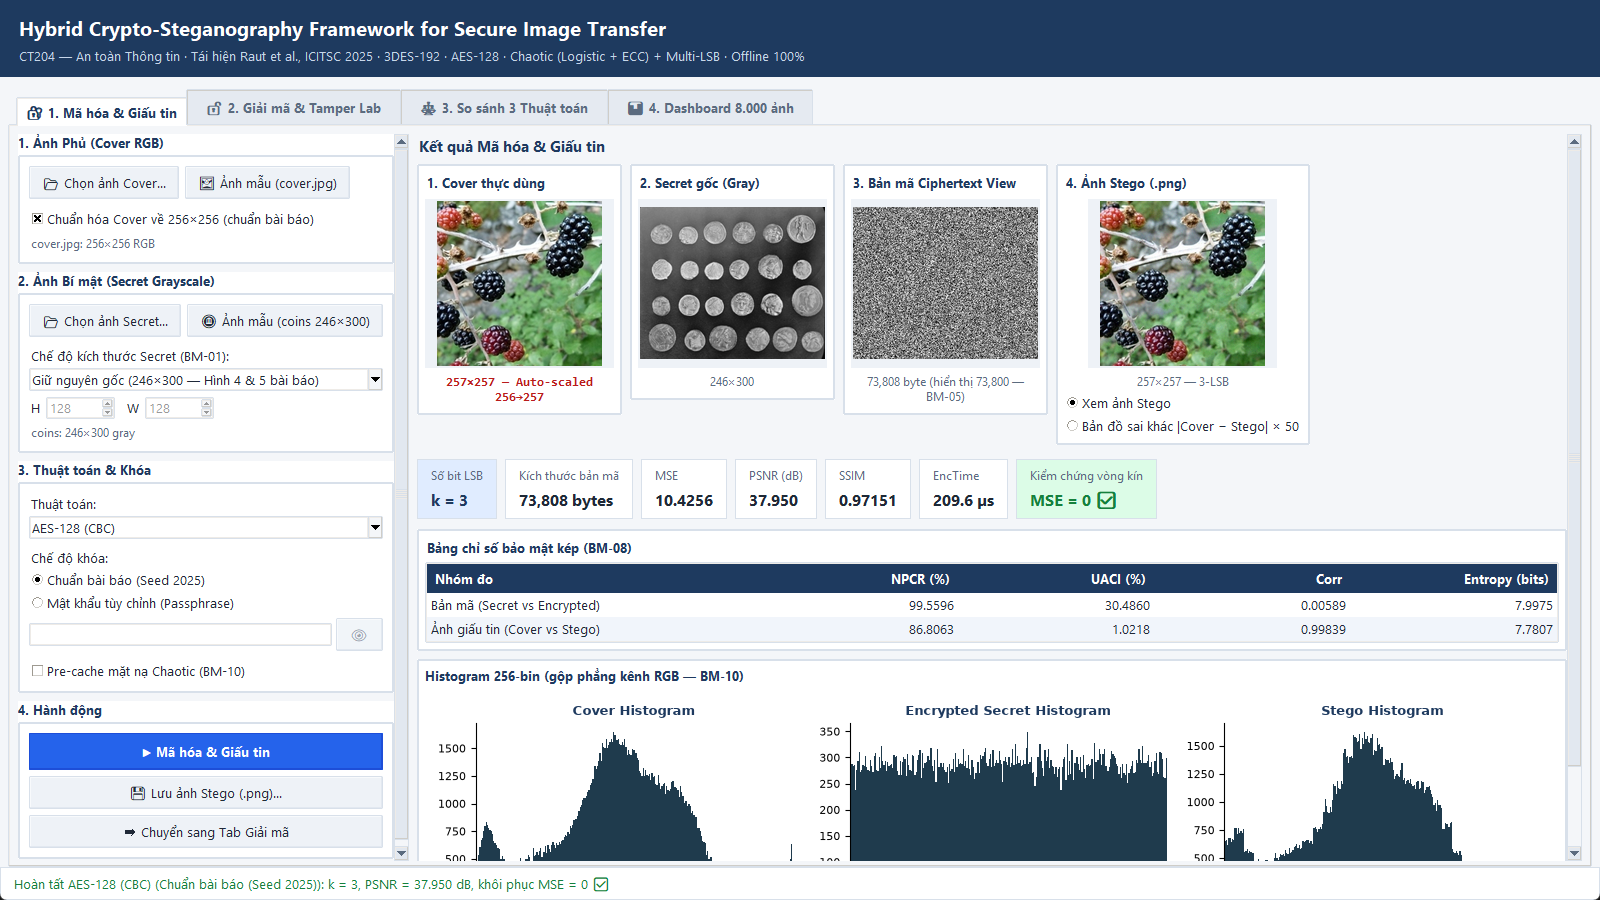
\includegraphics[width=\linewidth]{tab1_encrypt}
\caption{Tab 1 -- mã hóa AES-128 và giấu ảnh $246\times300$ (tự động chọn 3-LSB và phóng to ảnh
phủ lên $257\times257$)}
\label{fig:ui-tab1}
\end{figure}

\subsection{Tab 2 -- Giải mã và phòng thí nghiệm tấn công}

Tab 2 mô phỏng phía nhận: mở một ảnh stego bất kỳ (hoặc nhận trực tiếp từ Tab 1), đọc và hiển thị
từng trường của header kèm trạng thái kiểm tra CRC, rồi trích xuất và giải mã. Phần ``phòng thí
nghiệm tấn công'' (\tn{tamper lab}) cho phép áp dụng năm kịch bản lên ảnh stego: giải mã bằng sai
khóa, nén JPEG chất lượng 95, đảo một bit trong header, đảo 1\% bit LSB của vùng dữ liệu và cộng
nhiễu Gauss $\sigma = 2$. Hệ thống báo rõ quá trình dừng ở giai đoạn nào (header, trích xuất hay
giải mã) và vì sao (\hinh{fig:ui-tab2}).

\begin{figure}[H]
\centering
\begin{subfigure}{\linewidth}
  \centering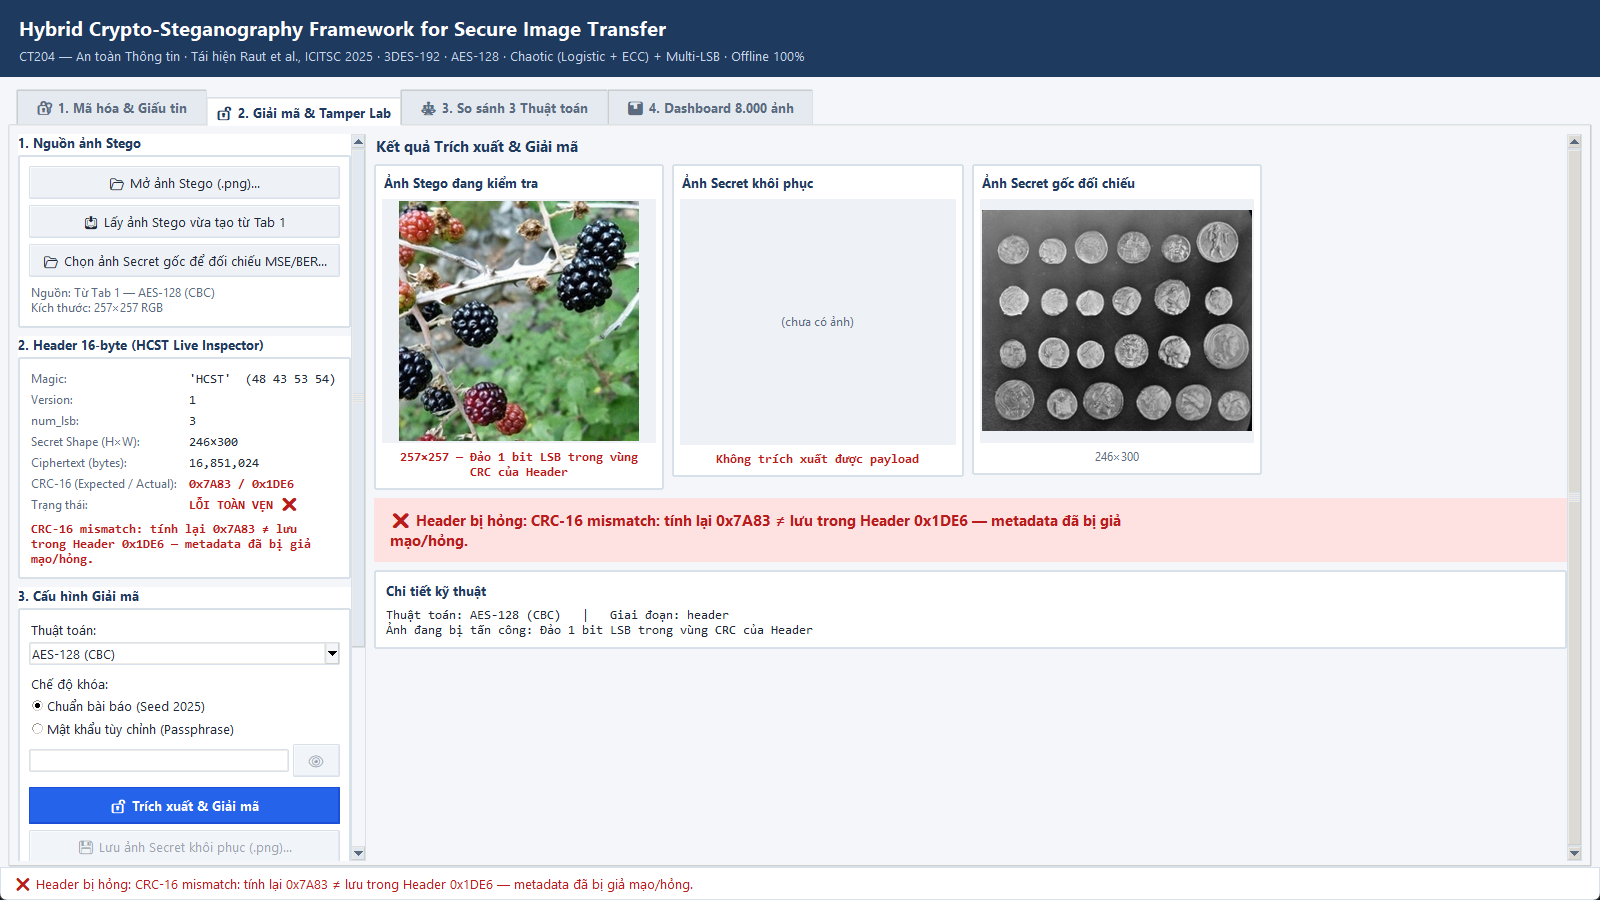
\includegraphics[width=0.93\linewidth]{tab2_tamper}
  \caption{Đảo 1 bit trong trường \code{ciphertext\_len}: magic vẫn đúng nhưng CRC-16 phát hiện
  header bị sửa}
\end{subfigure}

\vspace{3mm}
\begin{subfigure}{\linewidth}
  \centering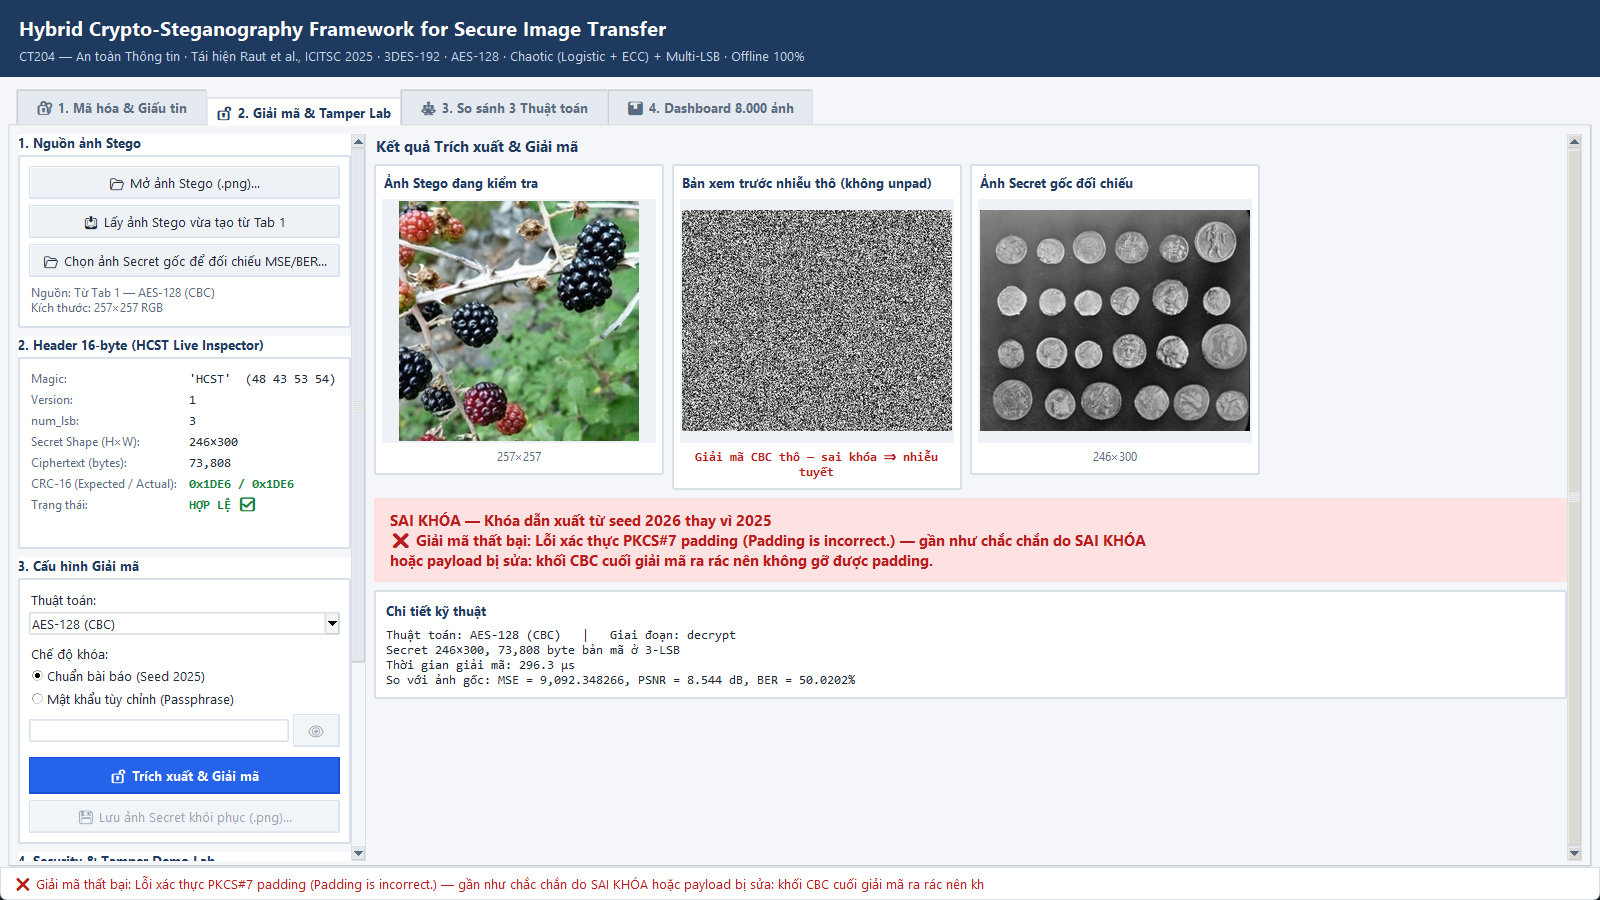
\includegraphics[width=0.93\linewidth]{tab2_wrongkey}
  \caption{Giải mã AES bằng khóa sai: lỗi gỡ đệm PKCS\#7, hiển thị dữ liệu giải mã thô (nhiễu)}
\end{subfigure}
\caption{Tab 2 -- kiểm tra header và phòng thí nghiệm tấn công}
\label{fig:ui-tab2}
\end{figure}

\subsection{Tab 3 -- So sánh ba thuật toán}

Tab 3 chạy cả ba thuật toán trên cùng một cặp ảnh và dựng lại Hình~5 của bài báo (ảnh mã hóa,
histogram bản mã, histogram ảnh stego của từng thuật toán), kèm bảng so sánh đầy đủ các độ đo và hệ
số tăng tốc so với 3DES (\hinh{fig:ui-tab3}). Toàn bộ kết quả có thể xuất ra thư mục dưới dạng ảnh
PNG và tệp CSV.

\begin{figure}[H]
\centering
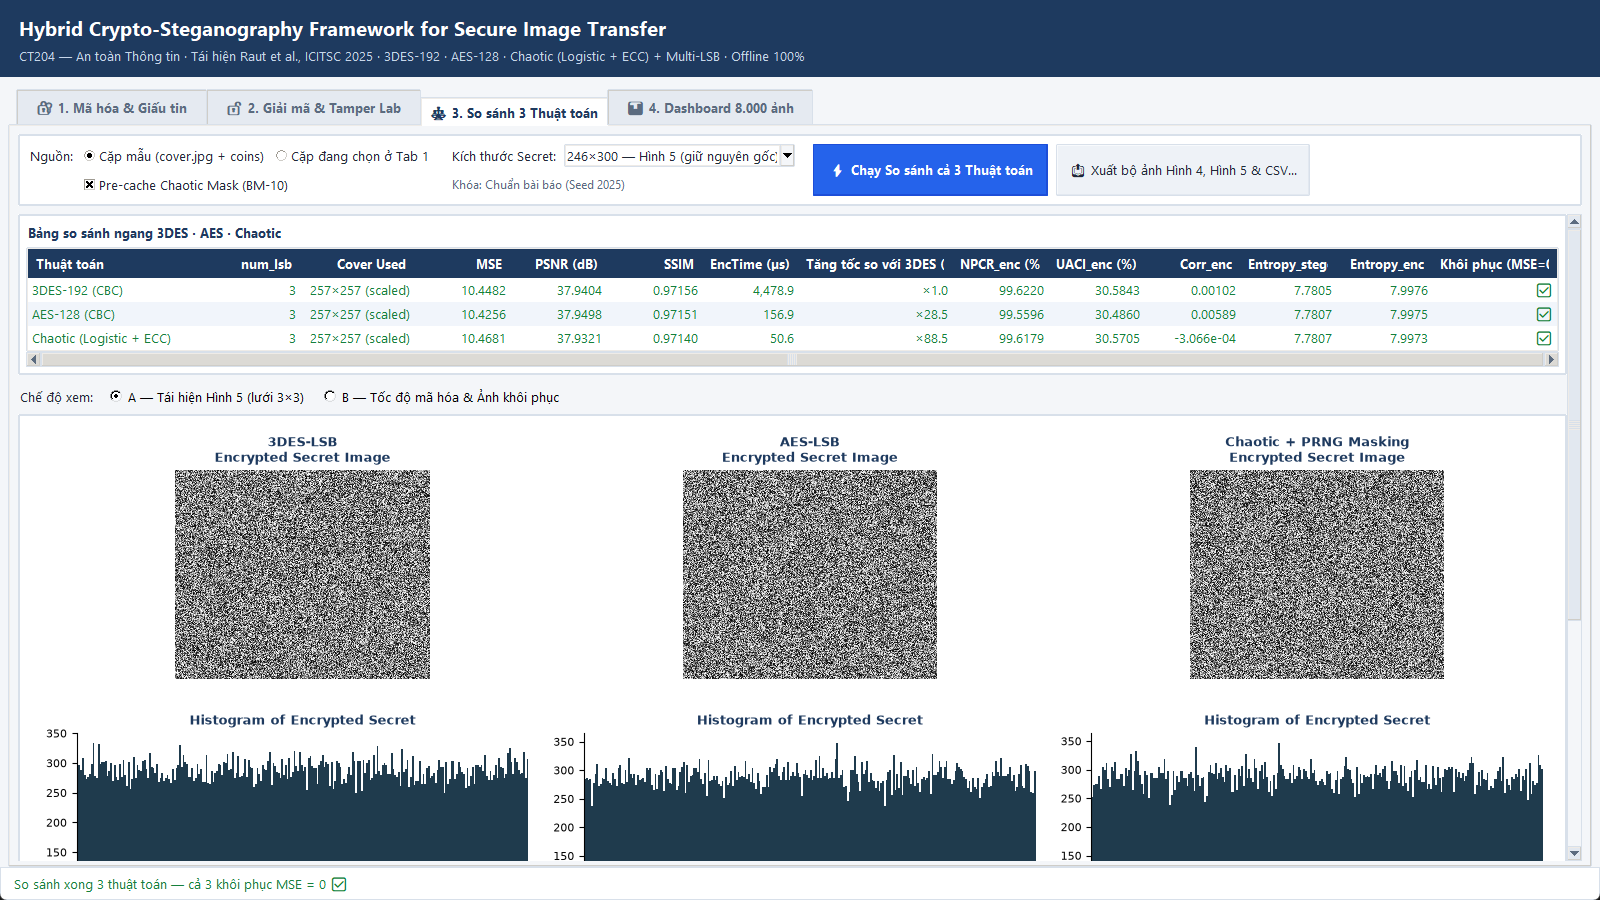
\includegraphics[width=\linewidth]{tab3_compare}
\caption{Tab 3 -- so sánh 3DES, AES và Chaotic trên cùng một cặp ảnh}
\label{fig:ui-tab3}
\end{figure}

\subsection{Tab 4 -- Bảng điều khiển kết quả 8000 ảnh}

Tab 4 nạp hai tệp CSV kết quả benchmark, hiển thị bảng đối chiếu ``Python -- bài báo -- chênh lệch''
cho từng thuật toán và các biểu đồ có thể lọc theo tập dữ liệu (\code{train}/\code{test}) và theo
lớp ảnh (\hinh{fig:ui-tab4}).

\begin{figure}[H]
\centering
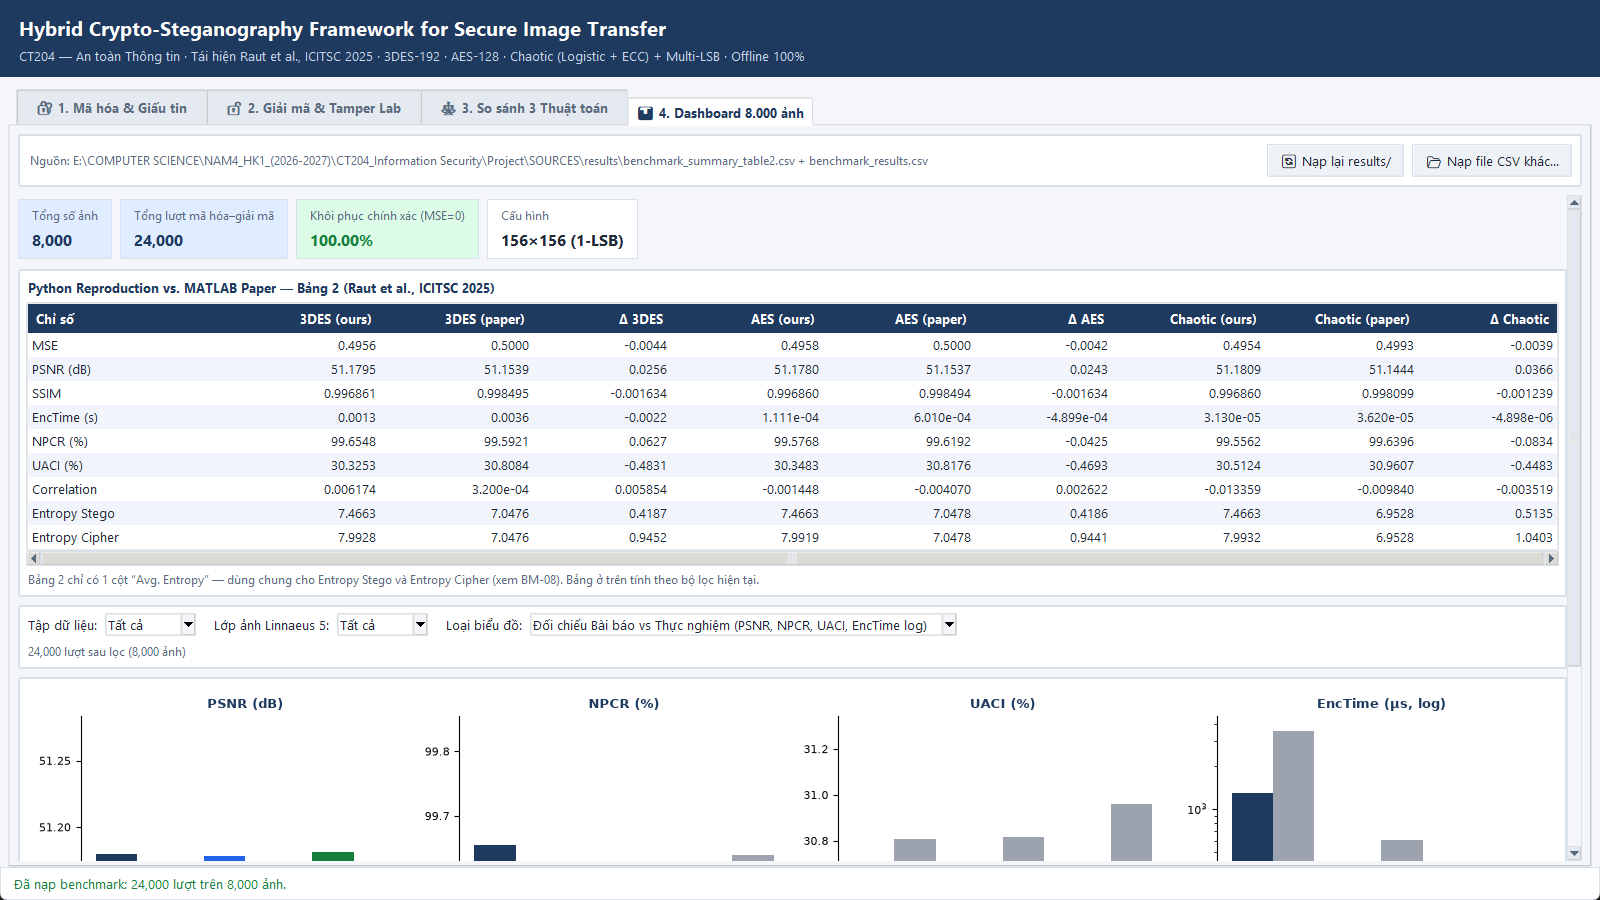
\includegraphics[width=\linewidth]{tab4_benchmark}
\caption{Tab 4 -- bảng điều khiển đối chiếu kết quả 8000 ảnh với Bảng~2 của bài báo}
\label{fig:ui-tab4}
\end{figure}

\subsection{Đóng gói thành tệp thực thi}

Ứng dụng được đóng gói bằng PyInstaller ở chế độ \emph{onedir} (\code{packaging/ct204\_app.spec}),
cho ra thư mục \code{CT204\_CryptoStego} gồm tệp \code{CT204\_CryptoStego.exe} và thư mục
\code{\_internal}. Gói kèm tệp cấu hình, cặp ảnh mẫu và các tệp kết quả benchmark, nhưng không kèm
8000 ảnh gốc. Khi chạy dạng \code{.exe}, ứng dụng tự xác định thư mục tài nguyên qua biến
\code{sys.\_MEIPASS} và chuyển bộ nhớ đệm JIT của Numba sang thư mục tạm để tránh lỗi ghi vào thư
mục chương trình. Người dùng chỉ cần giải nén và chạy, không cần cài Python.

\section{Kiểm thử phần mềm}

Hệ thống được kiểm thử tự động bằng pytest với tổng cộng \textbf{347 ca kiểm thử}
(\bang{tab:tests}). Toàn bộ 347 ca đều đạt khi chạy trên môi trường ở \bang{tab:tech}. Các ca kiểm
thử quan trọng nhất là kiểm thử khứ hồi (\tn{round-trip}): với mọi thuật toán, mọi kích thước ảnh
(kể cả ảnh toàn 0, ảnh có kích thước là bội số của 8/16, ảnh lớn buộc phải phóng to ảnh phủ), ảnh
khôi phục phải giống hệt ảnh gốc.

\begin{table}[H]
\centering
\caption{Thống kê các ca kiểm thử tự động}
\label{tab:tests}
\small
\begin{tabularx}{\linewidth}{@{}P{4.6cm}rL@{}}
\toprule
\thead{Tệp kiểm thử} & \thead{Số ca} & \thead{Nội dung chính}\\
\midrule
\code{test\_crypto.py}   & 126 & Khứ hồi cả 3 thuật toán; độ dài khóa/IV; đệm PKCS\#7; tính tất định; khóa 3DES suy biến; JIT warm-up; chế độ cache mặt nạ\\
\code{test\_lsb.py}      & 71  & Đóng gói/kiểm tra header, CRC; chọn $k$; công thức phóng to; nhúng/trích khứ hồi; phát hiện ảnh hỏng; không có vòng lặp Python trên điểm ảnh\\
\code{test\_metrics.py}  & 38  & MSE, PSNR, SSIM, NPCR, UACI, entropy, tương quan trên các ca đã biết đáp án; đo EncTime; chạy thử hai kịch bản \code{run\_single}, \code{run\_benchmark}\\
\code{test\_pipeline.py} & 40  & Đầu -- cuối: ảnh khôi phục giống hệt (MSE $=0$); ghi/đọc PNG; từ chối lưu JPEG\\
\code{test\_ui\_controller.py} & 72 & Nghiệp vụ giao diện: hai chế độ khóa, kiểm tra header, 4 kịch bản tấn công, xuất kết quả, luồng nền, chạy thử toàn bộ giao diện\\
\midrule
\textbf{Tổng} & \textbf{347} & \textbf{Tất cả đều đạt}\\
\bottomrule
\end{tabularx}
\end{table}

% =====================================================================
%  Chương 3 (tiếp) — Kết quả thực nghiệm và phân tích an toàn mở rộng
% =====================================================================

\section{Kết quả thực nghiệm}
\label{sec:ketqua}

\subsection{Dữ liệu, môi trường và kịch bản thực nghiệm}

Ảnh phủ là toàn bộ 8000 ảnh của bộ dữ liệu Linnaeus 5 \cite{chaladze2017}, gồm 5 lớp
(\hinh{fig:linnaeus}), mỗi lớp 1200 ảnh huấn luyện và 400 ảnh kiểm tra, kích thước $256\times256$.
Ảnh bí mật là ảnh xám ``coins'', lấy từ \code{skimage.data.coins()} và chuẩn hóa về kích thước
\code{coins.png} của MATLAB ($246\times300$) bằng nội suy \code{INTER\_AREA}. Cấu hình máy chạy thực
nghiệm được nêu ở \bang{tab:env}.

\begin{figure}[H]
\centering
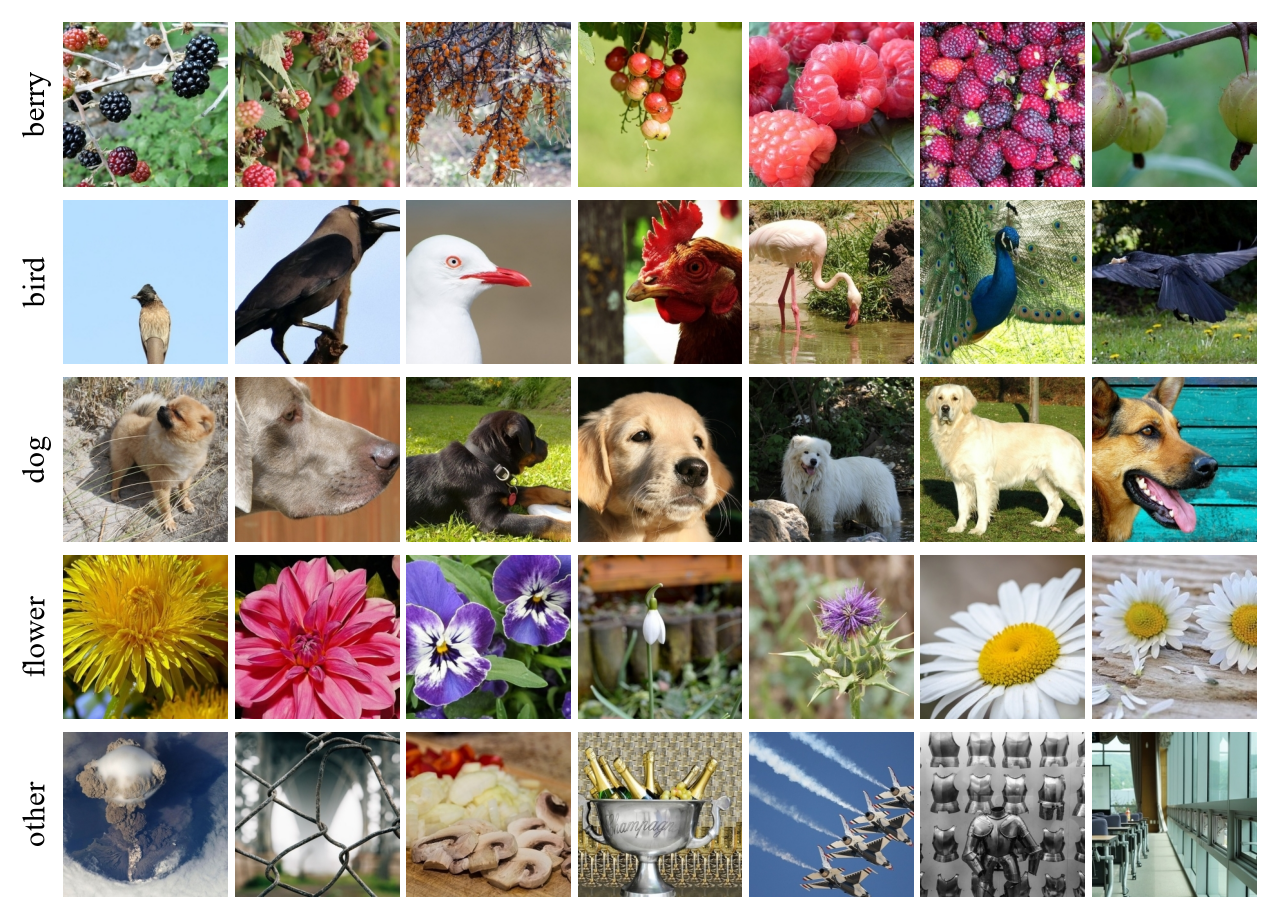
\includegraphics[width=0.86\linewidth]{linnaeus5_samples}
\caption{Một số ảnh phủ của bộ dữ liệu Linnaeus 5 (mỗi hàng là một lớp)}
\label{fig:linnaeus}
\end{figure}

\begin{table}[H]
\centering
\caption{Môi trường thực nghiệm}
\label{tab:env}
\small
\begin{tabularx}{0.85\linewidth}{@{}P{3.6cm}L@{}}
\toprule
\thead{Thành phần} & \thead{Cấu hình}\\
\midrule
Bộ xử lý & Intel Core i3-1005G1 (2 nhân, 4 luồng, xung cơ bản 1.20 GHz, hỗ trợ AES-NI)\\
Bộ nhớ & 20 GB RAM\\
Hệ điều hành & Windows 11 IoT Enterprise LTSC 2024 (64 bit)\\
Phần mềm & Python 3.12.8 và các thư viện ở \bang{tab:tech}\\
\bottomrule
\end{tabularx}
\end{table}

Theo quyết định BM-01, thực nghiệm được tổ chức thành hai kịch bản bổ sung cho nhau
(\bang{tab:scenarios}).

\begin{table}[H]
\centering
\caption{Hai kịch bản thực nghiệm}
\label{tab:scenarios}
\small
\begin{tabularx}{\linewidth}{@{}P{3.2cm}LL@{}}
\toprule
\thead{Thuộc tính} & \thead{Kịch bản A -- một cặp ảnh} & \thead{Kịch bản B -- benchmark}\\
\midrule
Mục đích & Tái hiện Hình~4 và Hình~5 & Tái hiện Bảng~2\\
Ảnh phủ & Ảnh mẫu \code{berry} & 8000 ảnh Linnaeus 5\\
Ảnh bí mật & $246\times300$ (\num{73800} byte) & $156\times156$ (\num{24336} byte)\\
Số bit LSB & 3 (ảnh phủ phóng to lên $257\times257$) & 1 (không phóng to)\\
Số lượt chạy & 3 (một lượt mỗi thuật toán) & \num{24000} ($8000 \times 3$)\\
Chaotic khi đo EncTime & Sinh lại mặt nạ mỗi lần & Cache mặt nạ (\code{--cache-chaotic-mask})\\
Kịch bản dòng lệnh & \code{scripts.run\_single} & \code{scripts.run\_benchmark --secret-size 156 156}\\
\bottomrule
\end{tabularx}
\end{table}

\subsection{Kết quả trên một cặp ảnh mẫu}

\hinh{fig:fig4} và \hinh{fig:fig5} là kết quả tái hiện Hình~4 và Hình~5 của bài báo. Histogram
ảnh phủ và ảnh bí mật (\hinh{fig:fig4}) có hình dạng tương tự bài báo: ảnh phủ có một đỉnh lớn
quanh mức 100--130, còn ảnh ``coins'' tập trung ở vùng tối 30--60 do nền ảnh. Ở \hinh{fig:fig5},
bản mã của cả ba thuật toán trông như nhiễu ngẫu nhiên, histogram phẳng với khoảng 288 điểm ảnh
mỗi mức, và histogram ảnh stego giữ nguyên hình dạng histogram ảnh phủ.

\begin{figure}[H]
\centering
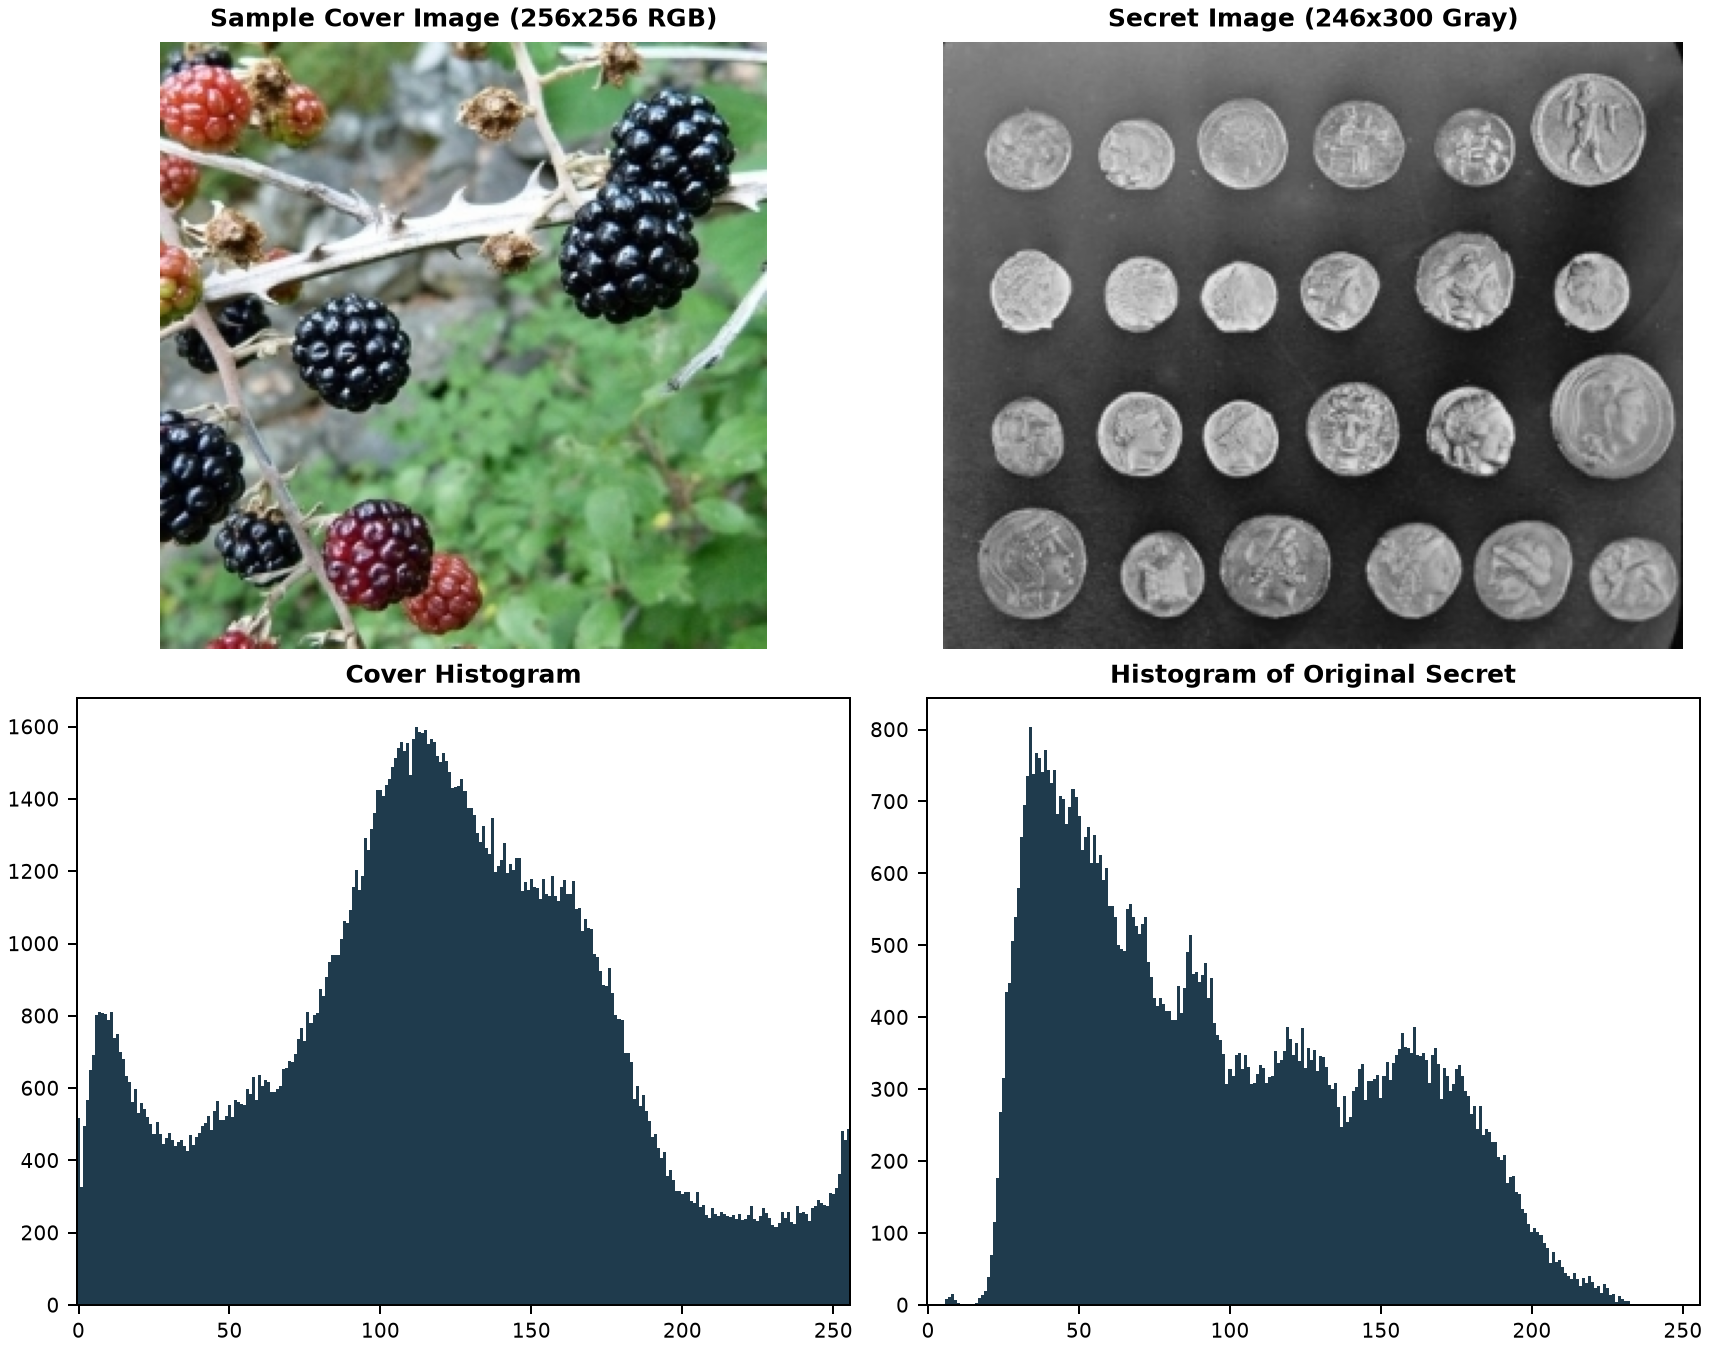
\includegraphics[width=0.82\linewidth]{fig4_cover_secret_histograms}
\caption{Tái hiện Hình~4 của bài báo: ảnh phủ, ảnh bí mật và histogram tương ứng}
\label{fig:fig4}
\end{figure}

\begin{figure}[H]
\centering
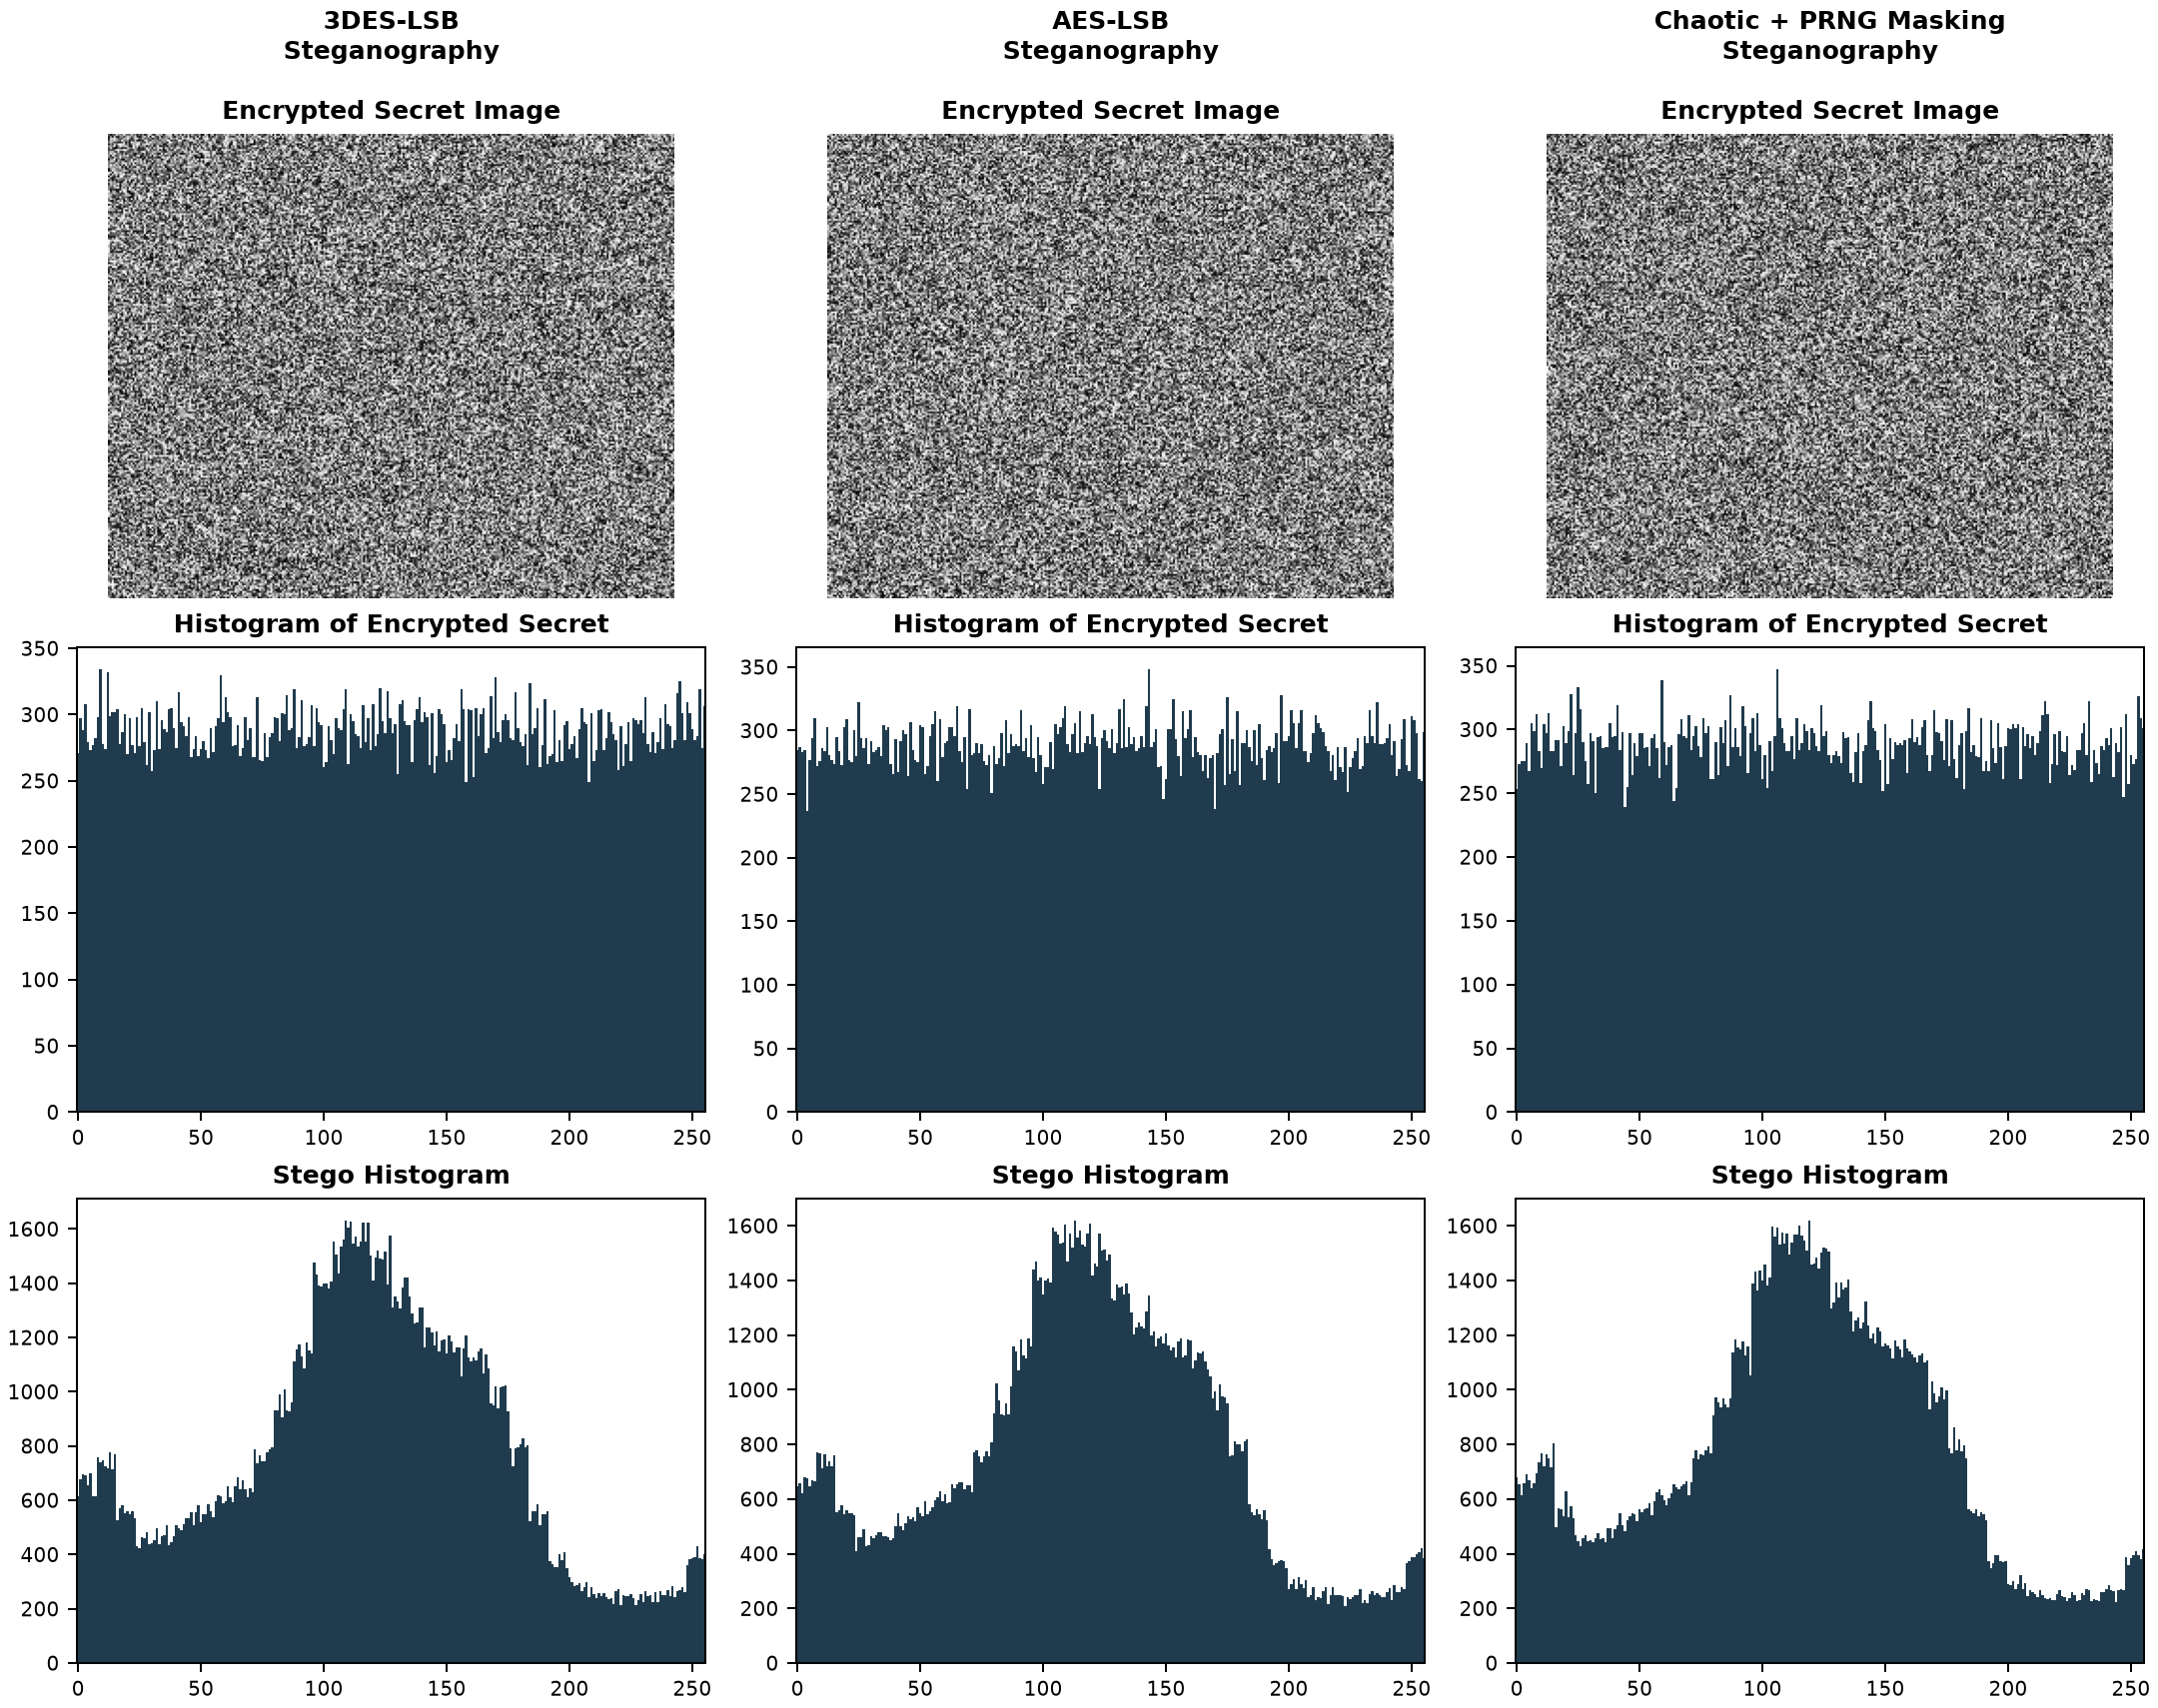
\includegraphics[width=0.92\linewidth]{fig5_comparison_grid}
\caption{Tái hiện Hình~5 của bài báo: bản mã, histogram bản mã và histogram ảnh stego của
3DES-LSB, AES-LSB và Chaotic-LSB (ảnh bí mật $246\times300$)}
\label{fig:fig5}
\end{figure}

\bang{tab:single} trình bày các độ đo của kịch bản A. Cả ba thuật toán đều khôi phục ảnh bí mật
chính xác tuyệt đối. Do tải tin \num{73800} byte vượt dung lượng 3-LSB của ảnh $256\times256$, hệ
thống tự động chọn $k = 3$ và phóng to ảnh phủ lên $257\times257$. MSE đo được ($\approx 10.43$)
khớp với giá trị lý thuyết $10.5\times99.3\%$ suy ra từ \pt{eq:lsb-mse}, trong đó $99.3\%$ là tỷ lệ
kênh màu thực sự được dùng. PSNR \SI{37.94}{dB} vẫn đủ cao để mắt thường không phân biệt được.

\begin{table}[H]
\centering
\caption{Kết quả kịch bản A -- ảnh bí mật $246\times300$, 3-LSB, ảnh phủ $257\times257$}
\label{tab:single}
\small
\begin{tabular}{@{}lrrr@{}}
\toprule
\thead{Độ đo} & \thead{3DES} & \thead{AES-128} & \thead{Chaotic}\\
\midrule
Độ dài bản mã (byte) & \num{73808} & \num{73808} & \num{73800}\\
MSE / PSNR (dB) & 10.448 / 37.94 & 10.426 / 37.95 & 10.468 / 37.93\\
SSIM & 0.97156 & 0.97151 & 0.97140\\
EncTime ($\mu$s) & \num{3587.7} & 285.1 & 834.5\\
NPCR\textsubscript{enc} / UACI\textsubscript{enc} (\%) & 99.622 / 30.584 & 99.560 / 30.486 & 99.618 / 30.570\\
Entropy bản mã (bit) & 7.99760 & 7.99751 & 7.99727\\
Khôi phục chính xác (MSE $= 0$) & \ok & \ok & \ok\\
\bottomrule
\end{tabular}
\end{table}

\hinh{fig:distortion} so sánh độ méo do nhúng ở hai mức tải tin. Ở 1-LSB, mỗi giá trị kênh thay đổi
nhiều nhất 1 đơn vị và chỉ $49.5\%$ số giá trị bị thay đổi (vì một nửa số bit nhúng tình cờ trùng
bit gốc). Ở 3-LSB, độ lệch tối đa là 7 và $86.8\%$ số giá trị bị thay đổi. Trong cả hai trường hợp,
bản đồ sai khác (đã khuếch đại) đều là nhiễu đều, không lộ đường nét của ảnh bí mật, nhờ bản mã có
phân bố bit ngẫu nhiên.

\begin{figure}[H]
\centering
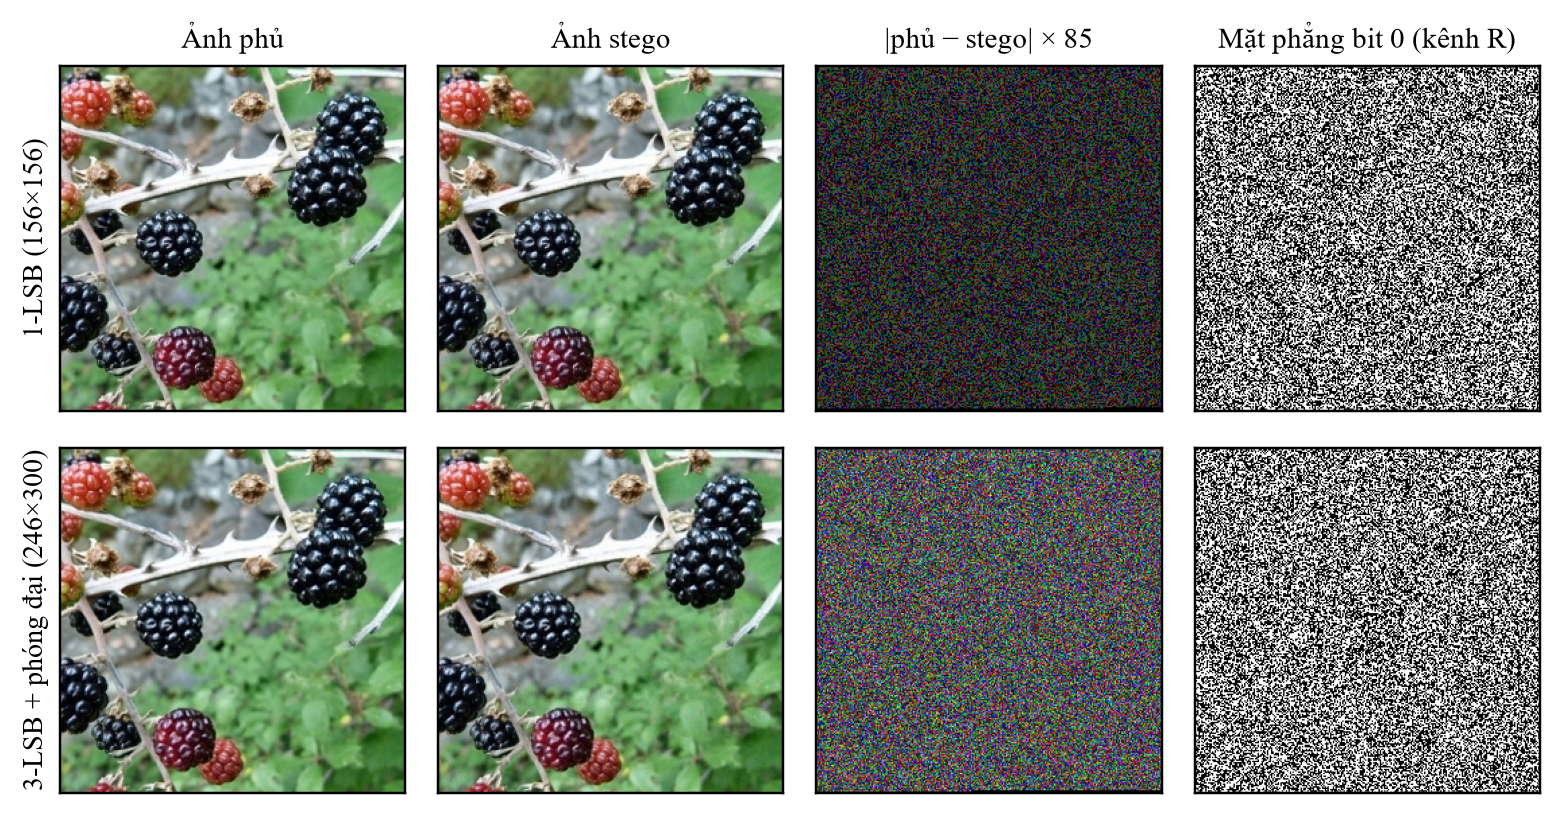
\includegraphics[width=\linewidth]{embedding_distortion}
\caption{Độ méo do nhúng: ảnh phủ, ảnh stego, sai khác tuyệt đối đã khuếch đại và mặt phẳng bit
thấp nhất (kênh R) ở hai mức tải tin}
\label{fig:distortion}
\end{figure}

\subsection{Chất lượng thị giác trên 8000 ảnh}

Ở kịch bản B, bản mã \num{24336}--\num{24352} byte cùng 128 bit header chiếm
$(128 + 8\cdot\num{24336}) / (3\cdot256^2) = 99.09\%$ số giá trị kênh. Theo \pt{eq:lsb-mse}, giá trị
kỳ vọng của MSE là $0.5\times0.9909 = 0.4954$, tương ứng PSNR $= \SI{51.18}{dB}$. Kết quả thực nghiệm
(\bang{tab:visual}, \hinh{fig:visual}) khớp gần như tuyệt đối với giá trị lý thuyết này. Toàn bộ
\num{24000} lượt chạy đều khôi phục ảnh bí mật chính xác và đều dùng 1-LSB.

\begin{table}[H]
\centering
\caption{Chất lượng thị giác trung bình trên 8000 ảnh (độ lệch chuẩn trong ngoặc)}
\label{tab:visual}
\small
\begin{tabular}{@{}llll@{}}
\toprule
\thead{Thuật toán} & \thead{MSE} & \thead{PSNR (dB)} & \thead{SSIM}\\
\midrule
3DES -- bài báo   & 0.499975 & 51.15389 & 0.998495\\
3DES -- tái hiện  & 0.495602 (0.0011) & 51.17948 (0.0099) & 0.996861 (0.0019)\\
AES -- bài báo    & 0.500006 & 51.15373 & 0.998494\\
AES -- tái hiện   & 0.495773 (0.0011) & 51.17798 (0.0098) & 0.996860 (0.0019)\\
Chaotic -- bài báo & 0.499321 & 51.14436 & 0.998099\\
Chaotic -- tái hiện & 0.495439 (0.0011) & 51.18092 (0.0097) & 0.996860 (0.0019)\\
\midrule
Lý thuyết (tải 99.09\%) & 0.4954 & 51.18 & --\\
\bottomrule
\end{tabular}
\end{table}

\begin{figure}[H]
\centering
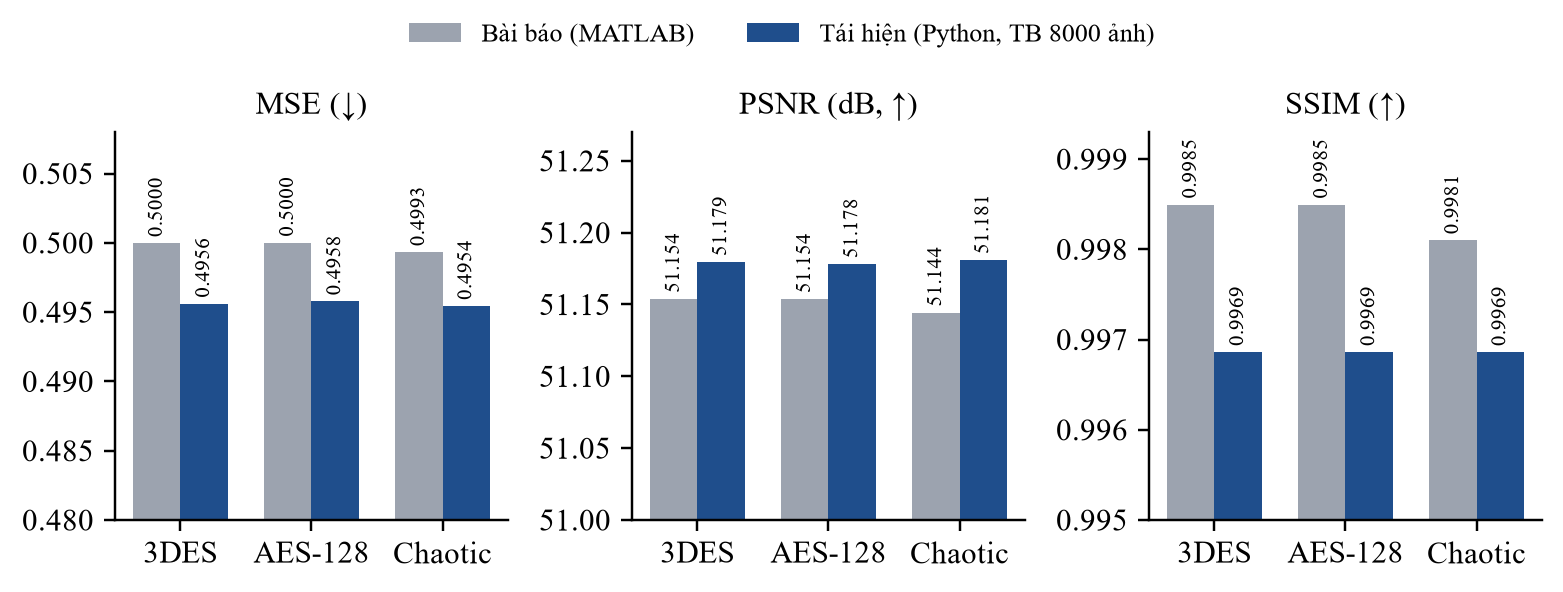
\includegraphics[width=\linewidth]{visual_paper_vs_ours}
\caption{So sánh MSE, PSNR, SSIM trung bình giữa bài báo và kết quả tái hiện}
\label{fig:visual}
\end{figure}

\begin{figure}[H]
\centering
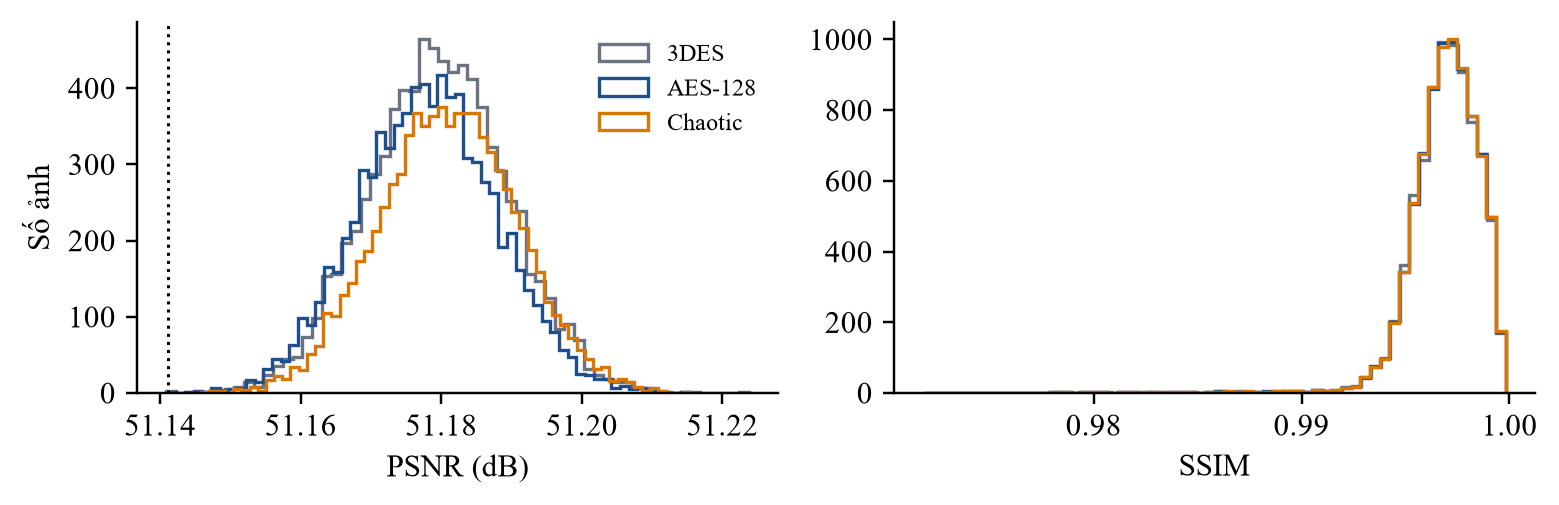
\includegraphics[width=\linewidth]{psnr_ssim_distribution}
\caption{Phân bố PSNR và SSIM trên 8000 ảnh (đường chấm: PSNR lý thuyết khi lấp đầy 100\% 1-LSB)}
\label{fig:psnr-dist}
\end{figure}

Nhận xét:
\begin{itemize}
  \item MSE và PSNR lệch bài báo dưới $1\%$ (PSNR lệch khoảng \SI{0.03}{dB}). Chênh lệch nhỏ này
        hoàn toàn do tỷ lệ lấp đầy: bài báo có MSE $\approx 0.5000$, tức đã lấp gần $100\%$ dung
        lượng 1-LSB, trong khi ảnh $156\times156$ lấp $99.09\%$.
  \item PSNR dao động rất hẹp (\SIrange{51.14}{51.22}{dB}) và gần như không phụ thuộc nội dung ảnh
        phủ hay thuật toán mã hóa, đúng như dự đoán từ \pt{eq:lsb-mse}: khi bit nhúng là ngẫu
        nhiên, độ méo chỉ phụ thuộc số bit nhúng.
  \item SSIM trung bình thấp hơn bài báo khoảng $0.0016$. Trên ảnh phủ đầu tiên (\code{berry}),
        SSIM đạt $0.99855$, gần như trùng giá trị $0.998495$ của bài báo; nhưng trên toàn bộ dữ liệu,
        các ảnh có vùng nền phẳng lớn (bầu trời, phông mờ) có SSIM thấp tới $0.972$ và kéo trung bình
        xuống. Bài báo không công bố cách tính SSIM cho ảnh màu nên không thể xác định chính xác
        nguyên nhân chênh lệch này.
\end{itemize}

\subsection{Độ an toàn thống kê của bản mã}
\label{sec:ketqua-antoan}

\bang{tab:enc-metrics} và \hinh{fig:dual} trình bày hai nhóm độ đo an toàn theo quyết định BM-08.
Một điểm quan trọng: vì khóa cố định và ảnh bí mật không đổi, bản mã của mỗi thuật toán \emph{giống
hệt nhau} trên cả 8000 lượt. Do đó các độ đo nhóm \code{*\_enc} thực chất là giá trị của một bản mã
duy nhất. Khác biệt NPCR giữa các thuật toán (ví dụ $99.59\%$ so với $99.64\%$ trong bài báo) chỉ là
dao động thống kê của một mẫu, không phản ánh thuật toán nào ``tốt hơn''.

\begin{table}[H]
\centering
\caption{Hai nhóm độ đo an toàn trung bình trên 8000 ảnh (ảnh bí mật $156\times156$)}
\label{tab:enc-metrics}
\small
\begin{tabular}{@{}lrrrr@{}}
\toprule
\thead{Độ đo} & \thead{3DES} & \thead{AES-128} & \thead{Chaotic} & \thead{Bài báo (AES)}\\
\midrule
\multicolumn{5}{@{}l}{\textit{Nhóm bản mã (ảnh bí mật -- bản mã)}}\\
NPCR\textsubscript{enc} (\%)    & 99.6548 & 99.5768 & 99.5562 & 99.6192\\
UACI\textsubscript{enc} (\%)    & 30.3253 & 30.3483 & 30.5124 & 30.8176\\
Tương quan\textsubscript{enc}   & 0.00617 & $-0.00145$ & $-0.01336$ & $-0.00407$\\
Entropy bản mã (bit)            & 7.99285 & 7.99189 & 7.99318 & --\\
\midrule
\multicolumn{5}{@{}l}{\textit{Nhóm ảnh stego (ảnh phủ -- ảnh stego)}}\\
NPCR\textsubscript{stego} (\%)  & 49.560 & 49.577 & 49.544 & --\\
UACI\textsubscript{stego} (\%)  & 0.1944 & 0.1944 & 0.1943 & --\\
Tương quan\textsubscript{stego} & 0.99989 & 0.99989 & 0.99989 & --\\
Entropy ảnh stego (bit)         & 7.46633 & 7.46633 & 7.46634 & 7.04776\\
\bottomrule
\end{tabular}
\end{table}

\begin{figure}[H]
\centering
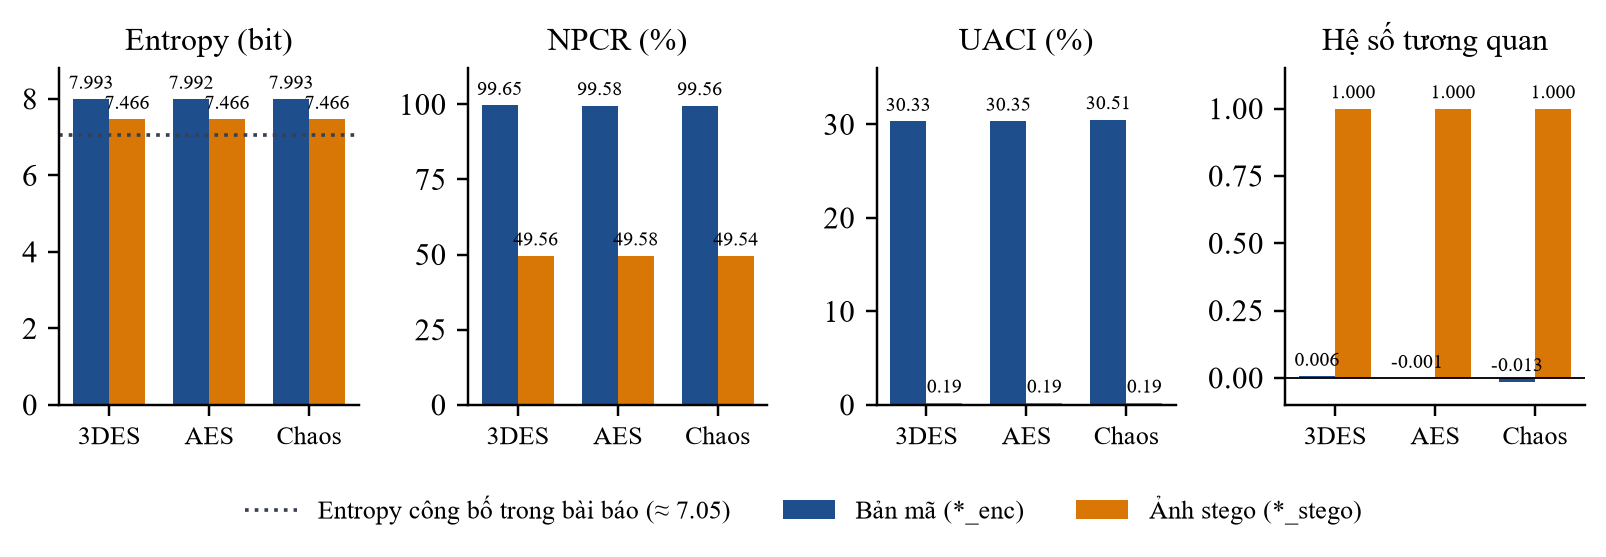
\includegraphics[width=\linewidth]{dual_metrics}
\caption{Hai nhóm độ đo: bản mã (\code{*\_enc}) và ảnh stego (\code{*\_stego})}
\label{fig:dual}
\end{figure}

Từ kết quả trên có thể giải thích đầy đủ các con số an toàn trong Bảng~2 của bài báo:
\begin{itemize}
  \item \textbf{NPCR} của cả ba thuật toán xấp xỉ giá trị lý thuyết $255/256 = 99.609\%$ của một
        bản mã ngẫu nhiên đều.
  \item \textbf{UACI} $\approx 30.3$--$30.5\%$, thấp hơn ngưỡng $33.46\%$ mà bài báo nêu. Đây
        \emph{không} phải dấu hiệu bản mã yếu. Khi so một ảnh bí mật cố định với một bản mã ngẫu
        nhiên đều $U$, giá trị kỳ vọng của UACI bằng
        $\frac{1}{mn}\sum_{i,j}\mathbb{E}\,|I(i,j) - U| / 255$ và phụ thuộc phân bố mức xám của
        ảnh bí mật. Tính trực tiếp trên ảnh ``coins'' $156\times156$ (độ sáng trung bình 96.9) cho
        giá trị kỳ vọng $30.41\%$, khớp với thực nghiệm. Ngưỡng $33.46\%$ chỉ đúng khi so hai ảnh
        ngẫu nhiên đều với nhau.
  \item \textbf{Entropy}: bản mã của cả ba thuật toán có entropy $\approx 7.992$--$7.993$ bit, sát
        cực đại 8. Giá trị $\approx 7.05$ trong bài báo nằm trong khoảng entropy của ảnh stego (ảnh
        màu tự nhiên, ở đây trung bình $7.47$), chứng tỏ bài báo đo entropy trên ảnh stego chứ
        không phải trên bản mã. Entropy của ảnh stego gần như bằng entropy của ảnh phủ và hầu như
        không phụ thuộc thuật toán mã hóa. Vì vậy kết luận của bài báo rằng Chaotic ``có entropy
        thấp hơn, cần nghiên cứu thêm về tính ngẫu nhiên'' không có cơ sở.
  \item \textbf{Tương quan} giữa ảnh bí mật và bản mã xấp xỉ 0 ở cả ba thuật toán, trong khi tương
        quan giữa ảnh phủ và ảnh stego là $0.9999$, phản ánh đúng vai trò của hai lớp: lớp mã hóa
        phá vỡ mọi liên hệ với bản rõ, lớp giấu tin giữ ảnh mang tin gần như không đổi.
\end{itemize}

Để đánh giá kỹ hơn tính ngẫu nhiên, em tính thêm tương quan giữa các điểm ảnh kề nhau và kiểm định
$\chi^2$ tính đều của histogram ($\chi^2 = \sum_i (o_i - e_i)^2/e_i$ với 255 bậc tự do, giá trị
tới hạn ở mức ý nghĩa $5\%$ là $293.25$). Kết quả ở \bang{tab:adjacent} và \hinh{fig:scatter} cho
thấy ảnh bí mật có tương quan điểm ảnh kề rất cao (0.89--0.94), còn bản mã của cả ba thuật toán có
tương quan xấp xỉ 0 và đều vượt qua kiểm định tính đều.

\begin{table}[H]
\centering
\caption{Tương quan điểm ảnh kề, entropy và kiểm định $\chi^2$ tính đều ($156\times156$)}
\label{tab:adjacent}
\small
\begin{tabular}{@{}lrrrrrc@{}}
\toprule
\thead{Ảnh} & \thead{Ngang} & \thead{Dọc} & \thead{Chéo} & \thead{Entropy} & \thead{$\chi^2$} & \thead{Đều?}\\
\midrule
Ảnh bí mật       & 0.92566 & 0.94084 & 0.88696 & 7.4252 & \num{15143.5} & \no\\
Bản mã 3DES      & $-0.00255$ & 0.00860 & 0.00398 & 7.9928 & 241.2 & \ok\\
Bản mã AES-128   & $-0.00565$ & $-0.00265$ & 0.01160 & 7.9919 & 272.3 & \ok\\
Bản mã Chaotic   & $-0.00211$ & 0.00702 & 0.00050 & 7.9932 & 231.9 & \ok\\
\bottomrule
\end{tabular}
\end{table}

\begin{figure}[H]
\centering
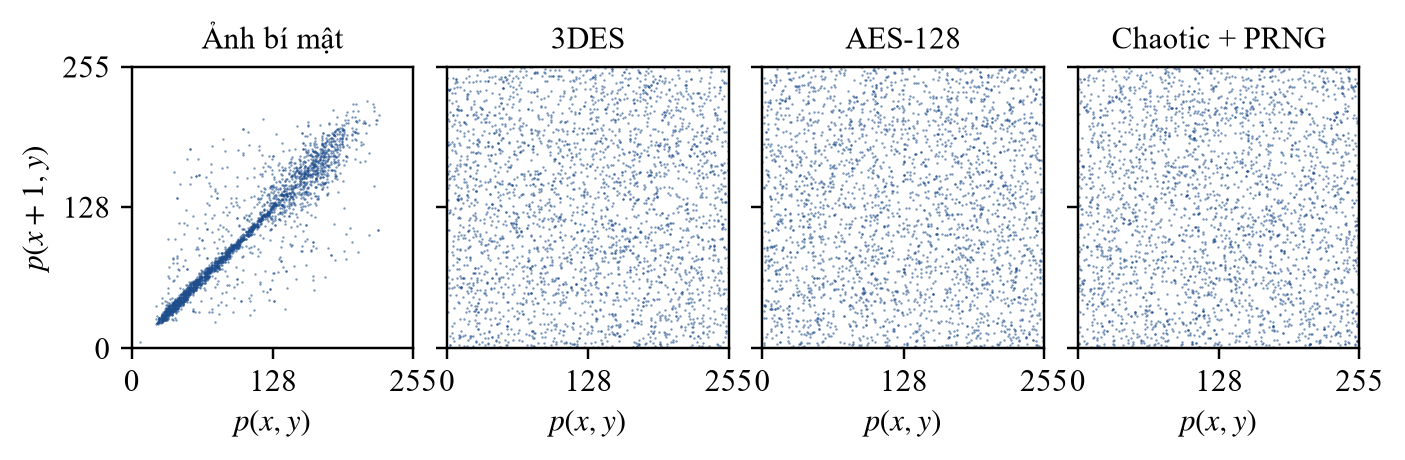
\includegraphics[width=\linewidth]{adjacent_scatter}
\caption{Phân bố cặp điểm ảnh kề theo chiều ngang (3000 cặp ngẫu nhiên)}
\label{fig:scatter}
\end{figure}

\subsection{Hiệu năng tốc độ mã hóa}

\bang{tab:enctime} và \hinh{fig:enctime} so sánh thời gian mã hóa với bài báo.

\begin{table}[H]
\centering
\caption{Thời gian mã hóa ($\mu$s) -- kịch bản B: 8000 lượt mỗi thuật toán}
\label{tab:enctime}
\small
\begin{tabular}{@{}lrrrrr@{}}
\toprule
\thead{Thuật toán} & \thead{Bài báo} & \thead{Trung bình} & \thead{Trung vị} & \thead{P95} & \thead{$246\times300$}\\
\midrule
3DES-192 CBC          & \num{3552} & \num{1303.1} & \num{1199.6} & \num{1602.2} & \num{3587.7}\\
AES-128 CBC           & 601        & 111.1        & 100.4        & 149.3        & 285.1\\
Chaotic + PRNG        & 36.2       & 31.3         & 26.0         & 51.3         & 834.5\textsuperscript{*}\\
\bottomrule
\multicolumn{6}{@{}l}{\footnotesize \textsuperscript{*} Không cache mặt nạ: thời gian gồm cả sinh \num{73800} giá trị Logistic và \num{73800} byte PRNG.}
\end{tabular}
\end{table}

\begin{figure}[H]
\centering
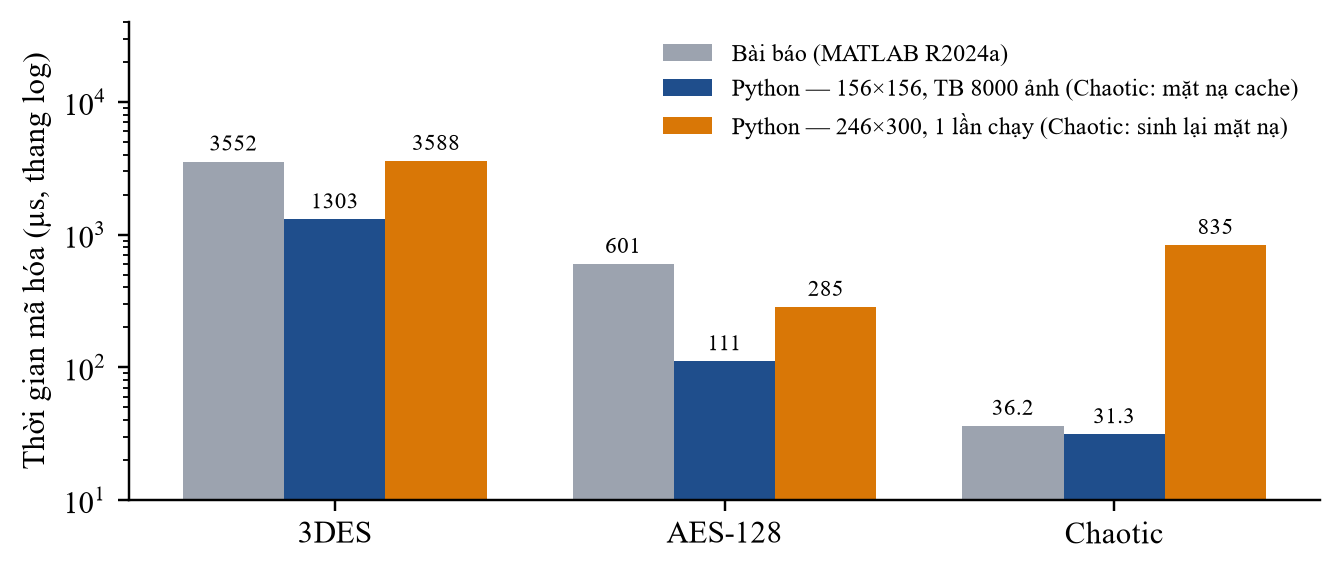
\includegraphics[width=0.9\linewidth]{enctime_compare}
\caption{Thời gian mã hóa: bài báo và kết quả tái hiện (thang logarit)}
\label{fig:enctime}
\end{figure}

\begin{figure}[H]
\centering
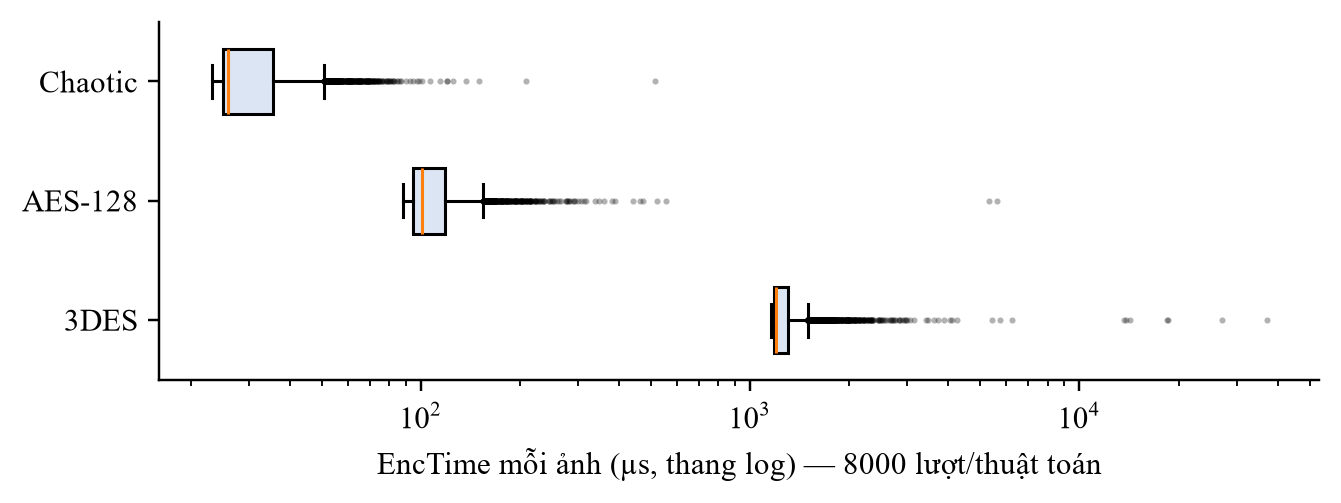
\includegraphics[width=0.9\linewidth]{enctime_distribution}
\caption{Phân bố thời gian mã hóa trên 8000 lượt chạy của mỗi thuật toán}
\label{fig:enctime-dist}
\end{figure}

Nhận xét:
\begin{itemize}
  \item Thứ tự tốc độ \textbf{Chaotic $<$ AES $<$ 3DES} của bài báo được tái hiện đúng. Với ảnh
        $156\times156$, Chaotic nhanh hơn 3DES khoảng $41.6$ lần và nhanh hơn AES khoảng $3.5$ lần;
        AES nhanh hơn 3DES khoảng $11.7$ lần.
  \item Thời gian 3DES trên ảnh $246\times300$ (\SI{3588}{\micro s}) gần như trùng giá trị
        \SI{3552}{\micro s} của bài báo. Điều này củng cố nhận định ở BM-01 rằng bài báo đo EncTime
        trên ảnh ``coins'' kích thước đầy đủ.
  \item AES trong bản tái hiện nhanh hơn bài báo khoảng $5.4$ lần nhờ PyCryptodome dùng tập lệnh
        phần cứng AES-NI. 3DES không có hỗ trợ phần cứng tương tự nên chậm hơn hẳn, vì phải chạy 48
        vòng Feistel trên khối 64 bit.
  \item Con số \SI{36.2}{\micro s} của Chaotic trong bài báo chỉ đạt được khi \emph{mặt nạ được tính
        sẵn} và chỉ đo phép XOR (chế độ cache: \SI{31.3}{\micro s}). Nếu tính cả chi phí sinh mặt nạ,
        Chaotic trên ảnh $246\times300$ mất \SI{834.5}{\micro s}, chậm hơn AES. Như vậy lợi thế tốc
        độ ``hai bậc độ lớn'' mà bài báo nêu phụ thuộc mạnh vào cách đo.
  \item Phân bố thời gian có đuôi dài (\hinh{fig:enctime-dist}) do ảnh hưởng của bộ lập lịch hệ điều
        hành và bộ nhớ đệm CPU; trung vị là đại lượng ổn định hơn trung bình khi so sánh.
\end{itemize}

\subsection{Phân tích theo lớp ảnh phủ}

Bài báo chỉ công bố giá trị trung bình gộp. Khi tách theo 5 lớp của Linnaeus 5
(\hinh{fig:class}), PSNR gần như không đổi nhưng SSIM và entropy ảnh stego khác nhau rõ rệt. Các
lớp nhiều kết cấu chi tiết như \code{dog} (SSIM $0.99721$, entropy $7.54$) và \code{berry}
($0.99709$; $7.51$) che giấu biến đổi LSB tốt hơn các lớp có nền phẳng như \code{flower}
($0.99653$) và \code{bird} ($0.99664$; entropy $7.37$). Nguyên nhân là SSIM nhạy với nhiễu $\pm1$
trên vùng phẳng hơn trên vùng nhiều chi tiết, gọi là hiệu ứng che lấp thị giác (\tn{visual
masking}). Kết quả trên tập \code{train} và \code{test} gần như trùng nhau (PSNR chênh dưới
\SI{0.001}{dB}, SSIM chênh dưới $0.0001$), cho thấy cỡ mẫu 8000 ảnh đủ để các giá trị trung bình
hội tụ.

\begin{figure}[H]
\centering
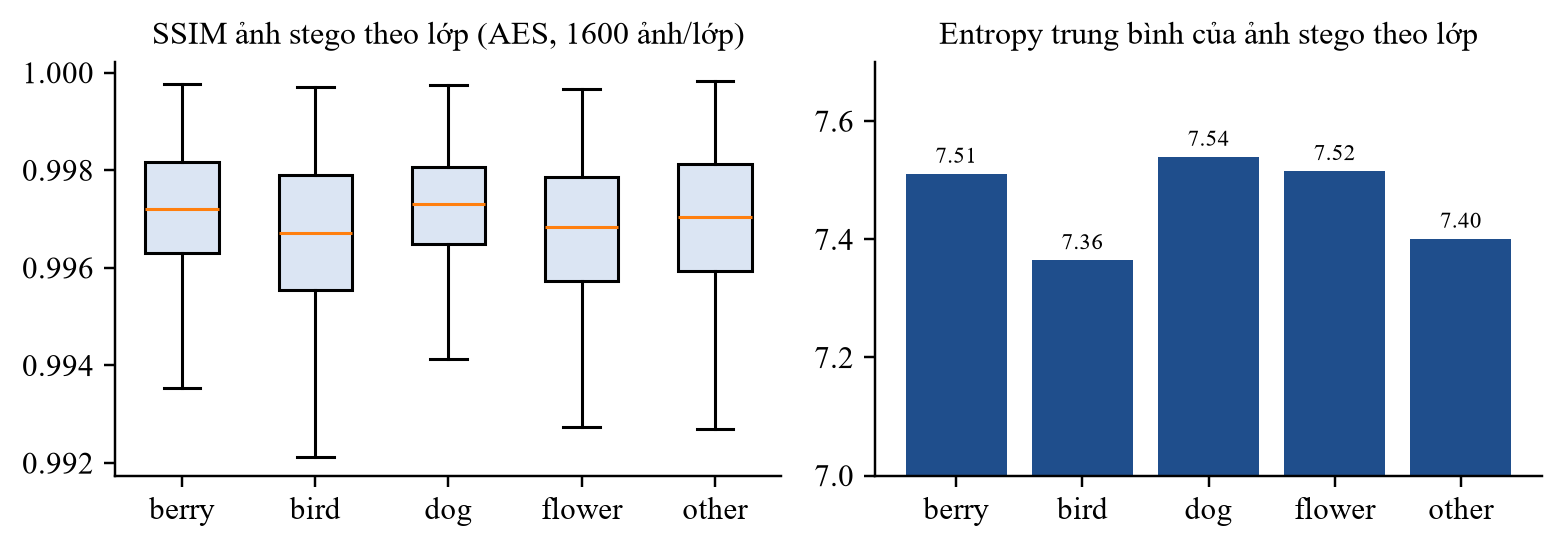
\includegraphics[width=\linewidth]{class_analysis}
\caption{SSIM và entropy ảnh stego theo 5 lớp ảnh phủ của Linnaeus 5}
\label{fig:class}
\end{figure}

\subsection{Đối chiếu tổng hợp với Bảng 2 của bài báo}

\bang{tab:compare-all} đặt cạnh nhau toàn bộ số liệu Bảng~2 của bài báo và kết quả tái hiện. Với
entropy, bản tái hiện đối chiếu cả hai cách đo.

\begin{table}[H]
\centering
\caption{Đối chiếu Bảng~2 của bài báo (BB) với kết quả tái hiện (TH) trên 8000 ảnh}
\label{tab:compare-all}
\footnotesize
\setlength{\tabcolsep}{4pt}
\begin{tabular}{@{}lrrrrrrl@{}}
\toprule
& \multicolumn{2}{c}{\thead{3DES}} & \multicolumn{2}{c}{\thead{AES-128}} & \multicolumn{2}{c}{\thead{Chaotic}} & \\
\cmidrule(lr){2-3}\cmidrule(lr){4-5}\cmidrule(lr){6-7}
\thead{Độ đo} & \thead{BB} & \thead{TH} & \thead{BB} & \thead{TH} & \thead{BB} & \thead{TH} & \thead{Mức khớp}\\
\midrule
MSE          & 0.49998 & 0.49560 & 0.50001 & 0.49577 & 0.49932 & 0.49544 & Rất sát\\
PSNR (dB)    & 51.1539 & 51.1795 & 51.1537 & 51.1780 & 51.1444 & 51.1809 & Rất sát\\
SSIM         & 0.99850 & 0.99686 & 0.99849 & 0.99686 & 0.99810 & 0.99686 & Sát\\
EncTime ($\mu$s) & 3552 & 1303 & 601 & 111 & 36.2 & 31.3 & Đúng thứ tự\\
NPCR (\%)    & 99.592 & 99.655 & 99.619 & 99.577 & 99.640 & 99.556 & Rất sát\\
UACI (\%)    & 30.808 & 30.325 & 30.818 & 30.348 & 30.961 & 30.512 & Sát, đúng thứ tự\\
Tương quan   & 0.0003 & 0.0062 & $-0.0041$ & $-0.0014$ & $-0.0098$ & $-0.0134$ & $\approx 0$\\
Entropy stego & 7.048 & 7.466 & 7.048 & 7.466 & 6.953 & 7.466 & Cùng đối tượng\\
Entropy bản mã & -- & 7.993 & -- & 7.992 & -- & 7.993 & Bài báo không đo\\
\bottomrule
\end{tabular}
\end{table}

Có thể kết luận bản tái hiện khớp với bài báo ở các điểm chính: MSE, PSNR, NPCR khớp gần như tuyệt
đối; UACI và SSIM khớp ở mức sát với chênh lệch đã được giải thích; thứ tự tốc độ được giữ nguyên.
Riêng entropy ảnh stego của bản tái hiện ($7.47$) cao hơn bài báo ($7.05$). Đây là đại lượng phụ
thuộc hoàn toàn vào ảnh phủ chứ không vào thuật toán, nên khác biệt có thể đến từ cách bài báo tính
entropy cho ảnh màu (ví dụ chuyển sang ảnh xám trước khi tính).

% =====================================================================
\section{Phân tích an toàn mở rộng}
\label{sec:antoan-morong}
% =====================================================================

Các độ đo trong bài báo chủ yếu mô tả \emph{tính thống kê} của bản mã và ảnh stego. Một hệ mật mã
chỉ có thể coi là an toàn khi chịu được các mô hình tấn công cụ thể. Phần này đánh giá thêm năm khía
cạnh mà bài báo chưa đề cập, dùng chính mã nguồn đã cài đặt và ảnh bí mật $156\times156$.

\subsection{Độ nhạy khóa}

Một hệ mật tốt phải cho bản mã khác hoàn toàn khi khóa thay đổi dù rất nhỏ, và giải mã bằng khóa
gần đúng không được tiết lộ thông tin. \bang{tab:keysens} cho thấy cả ba thuật toán đều đạt yêu cầu
này: đảo một bit khóa 3DES/AES, hay thay đổi $x_0$ hoặc $r$ chỉ $10^{-10}$, đều làm khoảng $99.3$--$99.6\%$
điểm ảnh bản mã thay đổi, UACI xấp xỉ $33.4\%$ (giá trị của hai ảnh ngẫu nhiên độc lập), và ảnh giải
mã bằng khóa sai chỉ còn là nhiễu (PSNR $\approx \SI{8.7}{dB}$). Với Chaotic, NPCR thấp hơn đôi chút
($99.3\%$) vì hai quỹ đạo Logistic chỉ tách nhau sau khoảng 30 bước lặp (\hinh{fig:logistic}b), nên
vài chục byte đầu của hai bản mã trùng nhau.

\begin{table}[H]
\centering
\caption{Độ nhạy khóa: so sánh bản mã của khóa đúng và khóa bị thay đổi rất nhỏ}
\label{tab:keysens}
\small
\begin{tabularx}{\linewidth}{@{}lLrrr@{}}
\toprule
\thead{Thuật toán} & \thead{Thay đổi khóa} & \thead{NPCR (\%)} & \thead{UACI (\%)} & \thead{PSNR giải mã sai}\\
\midrule
3DES    & Đảo 1 bit của $K_1$ (bit 1, byte 0) & 99.626 & 33.385 & \SI{8.61}{dB}\\
AES-128 & Đảo 1 bit của khóa (bit 0, byte 0)  & 99.552 & 33.466 & \SI{8.63}{dB}\\
Chaotic & $x_0 \to x_0 + 10^{-10}$            & 99.310 & 32.708 & \SI{8.72}{dB}\\
Chaotic & $r \to r + 10^{-10}$                & 99.240 & 32.771 & \SI{8.71}{dB}\\
Chaotic & \code{ecc\_seed}: $42 \to 43$       & 99.643 & 33.390 & \SI{8.72}{dB}\\
\bottomrule
\end{tabularx}
\end{table}

\subsection{Độ nhạy bản rõ -- phân tích vi sai đúng định nghĩa}

Trong phân tích vi sai chuẩn \cite{wu2011npcr}, kẻ tấn công mã hóa hai ảnh chỉ khác nhau \emph{một
điểm ảnh} rồi so sánh hai bản mã. Lược đồ tốt phải cho NPCR $\approx 99.6\%$ để không có quan hệ
khai thác được giữa thay đổi bản rõ và thay đổi bản mã. \bang{tab:plainsens} cho kết quả khi tăng
giá trị một điểm ảnh lên 1 ở ba vị trí khác nhau.

\begin{table}[H]
\centering
\caption{Độ nhạy bản rõ: NPCR/UACI (\%) giữa hai bản mã khi ảnh bí mật đổi đúng một điểm ảnh}
\label{tab:plainsens}
\small
\begin{tabular}{@{}lrrr@{}}
\toprule
\thead{Vị trí điểm ảnh thay đổi} & \thead{3DES} & \thead{AES-128} & \thead{Chaotic}\\
\midrule
Đầu ảnh $(0, 0)$        & 99.626 / 33.520 & 99.667 / 33.600 & 0.0041 / 0.00002\\
Giữa ảnh $(78, 78)$     & 49.511 / 16.594 & 49.466 / 16.483 & 0.0041 / 0.00005\\
Cuối ảnh $(155, 155)$   & 0.0329 / 0.0151 & 0.0657 / 0.0272 & 0.0041 / 0.00008\\
\bottomrule
\end{tabular}
\end{table}

Kết quả phản ánh đúng cấu trúc của từng thuật toán:
\begin{itemize}
  \item Với CBC, thay đổi ở khối $P_i$ lan sang mọi khối \emph{phía sau} theo \pt{eq:cbc}. Thay đổi
        điểm ảnh đầu làm toàn bộ bản mã thay đổi, ở giữa ảnh thì khoảng một nửa, còn ở điểm ảnh cuối
        thì chỉ đúng một khối thay đổi (8 byte $= 0.033\%$ với 3DES, 16 byte $= 0.066\%$ với AES).
  \item Với Chaotic + PRNG, dòng khóa không phụ thuộc bản rõ nên thay đổi một điểm ảnh chỉ làm
        \emph{đúng một byte} bản mã thay đổi ($1/\num{24336} = 0.0041\%$). Lược đồ hoàn toàn không có
        tính khuếch tán.
\end{itemize}
Như vậy, NPCR $\approx 99.6\%$ trong bài báo (đo giữa ảnh bí mật và bản mã) \emph{không} chứng minh
được khả năng chống tấn công vi sai. Khi đo đúng định nghĩa, Chaotic thất bại hoàn toàn, còn 3DES và
AES ở chế độ CBC với IV cố định chỉ đạt yêu cầu khi thay đổi nằm ở đầu ảnh.

\subsection{Tấn công biết bản rõ lên lớp Chaotic + PRNG}

Mặt nạ của lớp Chaotic được sinh từ các tham số cố định $(x_0, r, \mathit{seed})$, không phụ thuộc
bản rõ và không có số dùng một lần (\tn{nonce}). Vì vậy mọi ảnh đều được XOR với \emph{cùng một dòng
khóa} và lược đồ rơi vào đúng trường hợp dùng lại dòng khóa ở \pt{eq:twotime}. Em mô phỏng một kẻ tấn
công biết một cặp (ảnh bí mật $A$, bản mã $C_A$), ví dụ một ảnh đã từng bị lộ, và thu được bản mã
$C_B$ của một ảnh khác $B$ (ảnh ``camera''). Kết quả ở \hinh{fig:kpa}:
\begin{itemize}
  \item Chỉ cần XOR hai bản mã, $C_A \xor C_B = A \xor B$ đã lộ rõ đường nét chồng lên nhau của cả
        hai ảnh (hệ số tương quan với $A \xor B$ bằng $1.0$);
  \item Dòng khóa khôi phục được bằng $A \xor C_A$, từ đó giải mã được $B = C_B \xor (A \xor C_A)$
        \textbf{chính xác 100\%} mà không cần biết $x_0$, $r$ hay seed;
  \item Cùng phép tấn công đó với AES-CBC chỉ cho ra nhiễu (PSNR \SI{7.84}{dB}, tương quan $0.005$),
        vì AES là hoán vị giả ngẫu nhiên chứ không phải phép XOR với dòng khóa cố định.
\end{itemize}

\begin{figure}[H]
\centering
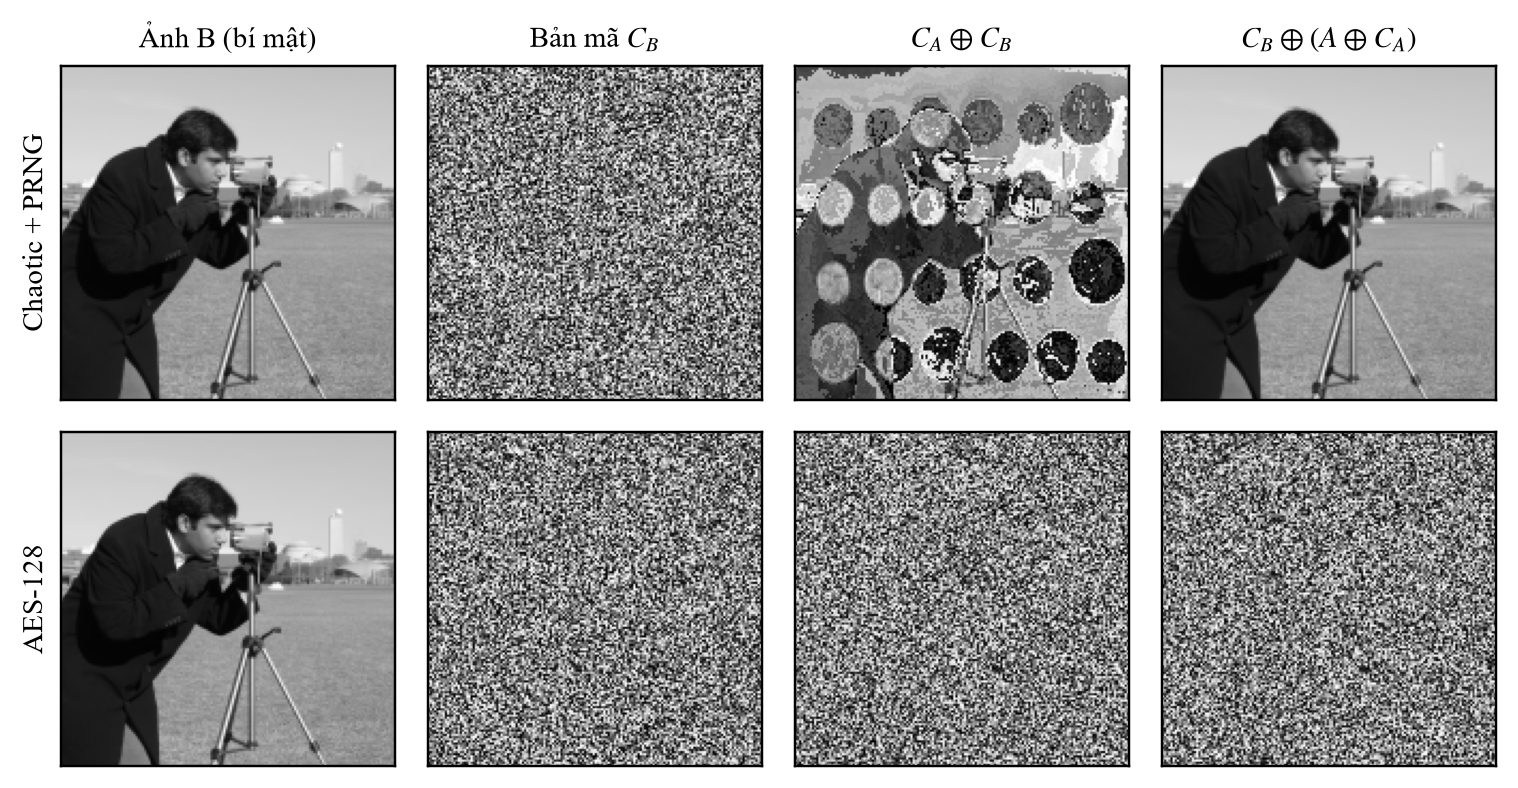
\includegraphics[width=0.95\linewidth]{kpa_attack}
\caption{Tấn công biết bản rõ: lớp Chaotic + PRNG bị phá hoàn toàn, AES-CBC không bị ảnh hưởng}
\label{fig:kpa}
\end{figure}

Ngoài ra, bài báo công bố công khai $x_0 = 0.785398$, $r = 3.999$, và mặt nạ ``ECC'' chỉ phụ thuộc
một seed số nguyên. Không gian khóa thực tế vì thế rất nhỏ so với 112 bit của 3DES hay 128 bit của
AES, vi phạm cả nguyên lý Kerckhoffs lẫn các yêu cầu cơ bản cho hệ mật hỗn loạn mà Alvarez và Li đã
nêu \cite{alvarez2006}. Kết luận rằng phương pháp hỗn loạn ``an toàn và nhanh hơn'' của bài báo vì
vậy cần được hiểu thận trọng: nó nhanh hơn chính vì nó chỉ là một mã dòng đơn giản dùng lại khóa.

\subsection{Khả năng chống chỉnh sửa}

Dùng phòng thí nghiệm tấn công của ứng dụng (Tab~2), em áp dụng năm kịch bản lên ảnh stego của cả ba
thuật toán. Kết quả tổng hợp ở \bang{tab:tamper} và \hinh{fig:tamper}.

\begin{table}[H]
\centering
\caption{Phản ứng của hệ thống trước các kịch bản tấn công/chỉnh sửa ảnh stego}
\label{tab:tamper}
\small
\begin{tabularx}{\linewidth}{@{}P{3.3cm}P{2.5cm}LL@{}}
\toprule
\thead{Kịch bản} & \thead{Dừng ở bước} & \thead{3DES / AES-128} & \thead{Chaotic}\\
\midrule
Không tấn công & -- & Khôi phục chính xác & Khôi phục chính xác\\
Giải mã sai khóa (seed + 1) & Giải mã & Phát hiện: lỗi gỡ đệm PKCS\#7; dữ liệu thô là nhiễu (PSNR 8.66/8.67 dB) & Không phát hiện: trả về ảnh nhiễu như kết quả hợp lệ (PSNR 8.72 dB)\\
Nén JPEG Q = 95 & Header & \multicolumn{2}{l}{Phát hiện: sai magic \code{HCST}, toàn bộ LSB bị phá hủy}\\
Đảo 1 bit trong header & Header & \multicolumn{2}{l}{Phát hiện: CRC-16 không khớp}\\
Đảo 1\% bit payload & Giải mã & Lỗi lan truyền theo khối: BER 24.1\% / 35.9\%, PSNR 11.9 / 10.0 dB; lần này lỗi đệm báo hiệu & Không phát hiện: BER đúng 1.0\%, PSNR 24.9 dB, lỗi rải rác\\
Nhiễu Gauss $\sigma = 2$ & Header & \multicolumn{2}{l}{Phát hiện: sai magic \code{HCST}}\\
\bottomrule
\end{tabularx}
\end{table}

\begin{figure}[H]
\centering
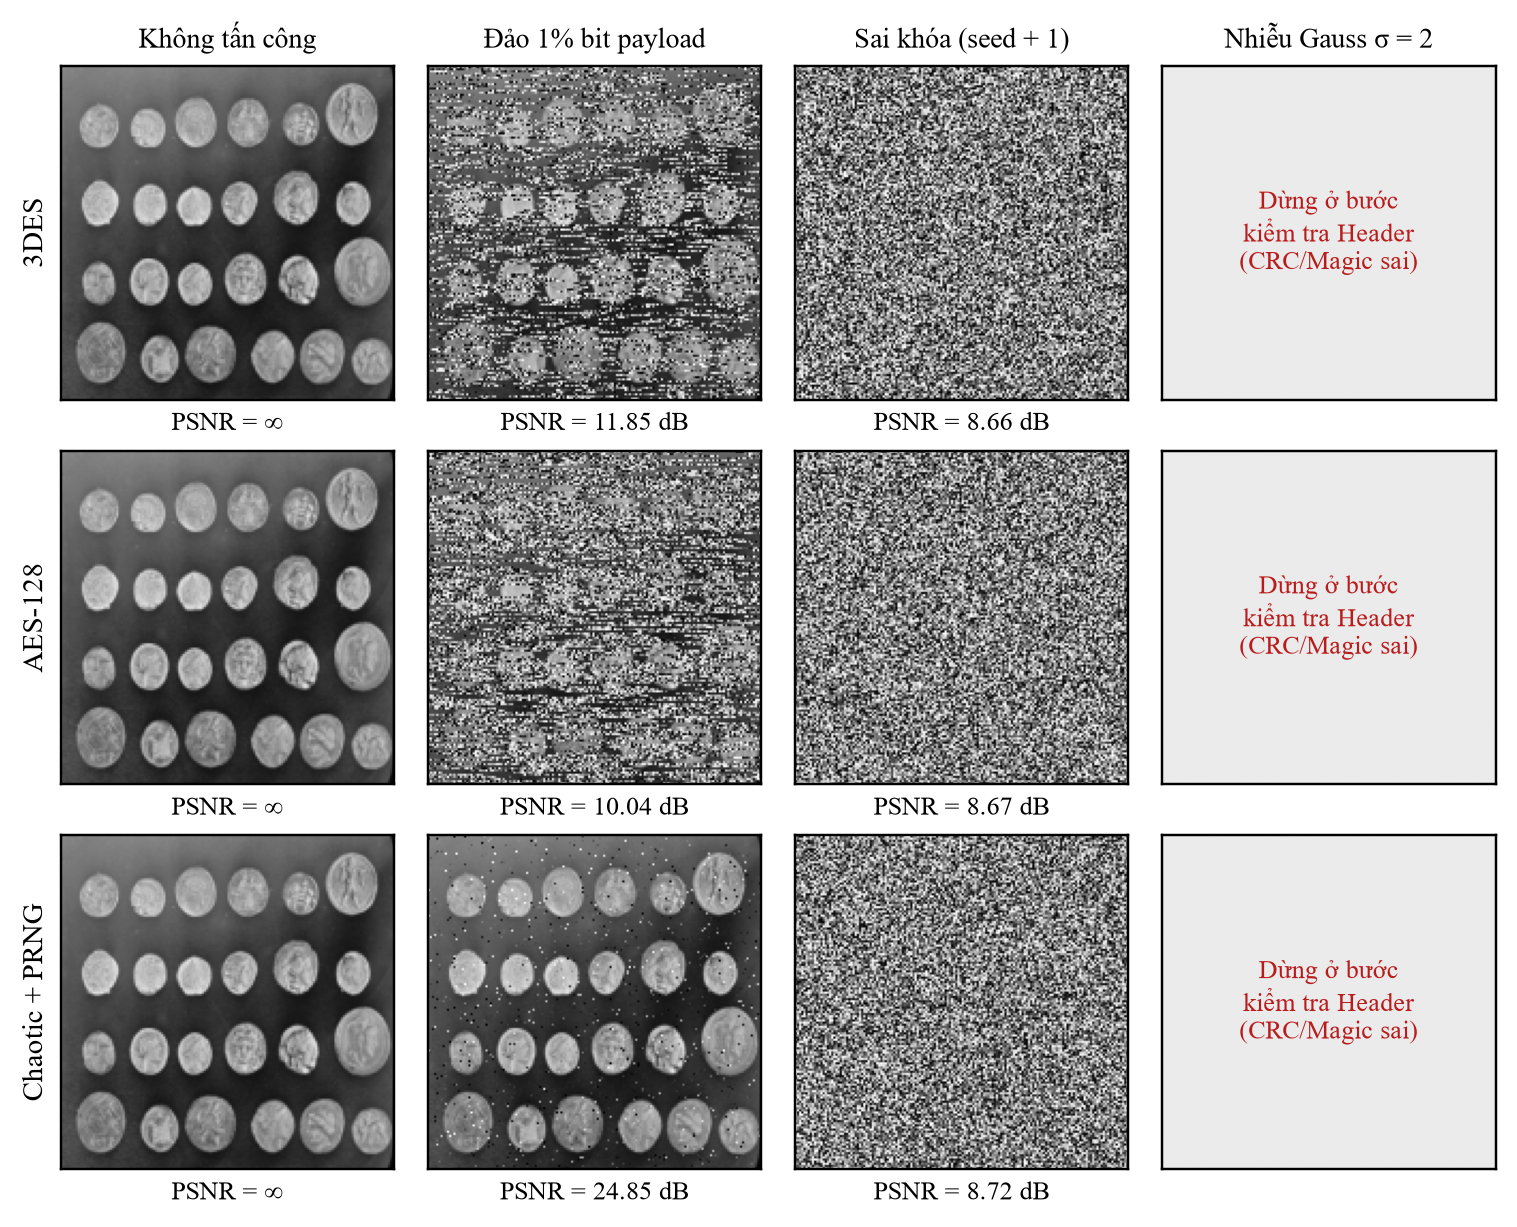
\includegraphics[width=0.92\linewidth]{tamper_grid}
\caption{Ảnh khôi phục dưới các kịch bản tấn công (cột cuối: bị chặn ngay ở bước kiểm tra header)}
\label{fig:tamper}
\end{figure}

Những nhận xét rút ra:
\begin{itemize}
  \item Giấu tin LSB thay thế là kỹ thuật \emph{mong manh} (\tn{fragile}): chỉ một lần nén JPEG chất
        lượng cao hoặc nhiễu rất nhỏ cũng phá hủy toàn bộ thông điệp. Header có magic và CRC-16 giúp
        hệ thống phát hiện ngay các trường hợp này thay vì giải mã ra dữ liệu rác, nhưng không khôi
        phục được thông điệp.
  \item CRC-16 chỉ phát hiện sai lệch ngẫu nhiên. Kẻ tấn công chủ động có thể sửa header rồi tính
        lại CRC. Phần payload hoàn toàn không được bảo vệ toàn vẹn: với 3DES/AES, việc phát hiện chỉ
        là ``tình cờ'' khi khối cuối bị hỏng làm sai đệm PKCS\#7; với Chaotic thì không có bất kỳ cơ
        chế phát hiện nào.
  \item Ở khía cạnh độ bền, Chaotic lại có ưu điểm: lỗi bit không lan truyền nên ảnh khôi phục vẫn
        nhận ra được (PSNR \SI{24.9}{dB}), trong khi CBC khuếch đại mỗi bit lỗi thành cả một khối
        hỏng.
\end{itemize}

\subsection{Khả năng bị phát hiện bởi phân tích giấu tin}

Mục tiêu cốt lõi của lớp giấu tin là không bị phát hiện. Tuy nhiên, ở chế độ 1-LSB lấp $99\%$ dung
lượng, mặt phẳng bit thấp nhất của ảnh stego bị thay hoàn toàn bằng dữ liệu ngẫu nhiên
(\hinh{fig:lsb-plane}). Trong khi đó mặt phẳng bit thấp của ảnh tự nhiên vẫn còn mang dấu vết cấu trúc
của ảnh, đặc biệt ở các vùng bão hòa hoặc phẳng.

\begin{figure}[H]
\centering
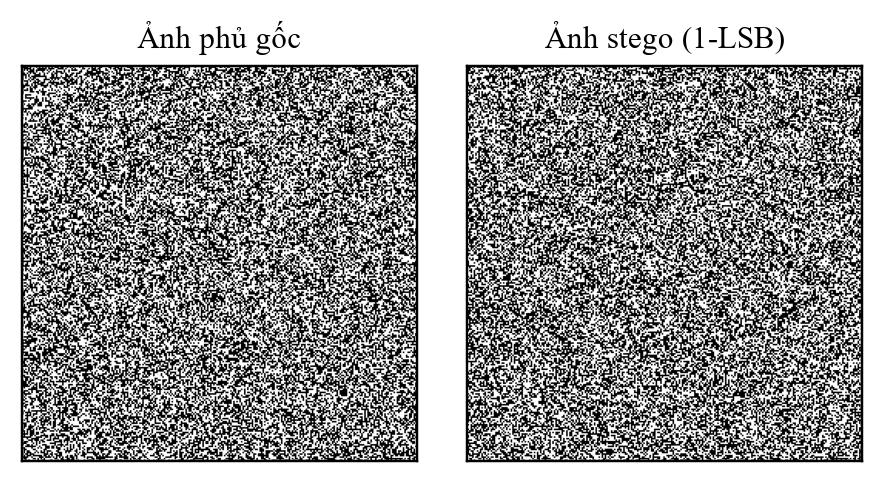
\includegraphics[width=0.62\linewidth]{lsb_plane}
\caption{Mặt phẳng bit thấp nhất (kênh R) của ảnh phủ và ảnh stego}
\label{fig:lsb-plane}
\end{figure}

Em áp dụng kiểm định $\chi^2$ trên cặp giá trị của Westfeld và Pfitzmann \cite{westfeld2000} cho cả
8000 ảnh phủ và 8000 ảnh stego tương ứng (AES, $156\times156$). Ảnh được coi là ``có giấu tin'' khi
giá trị $p > 0.95$. Kết quả (\hinh{fig:chi2}):
\begin{itemize}
  \item \textbf{99.84\%} ảnh stego bị phát hiện (trung vị $p = 0.999999$);
  \item chỉ \textbf{4.58\%} ảnh phủ gốc bị báo nhầm (trung vị $p \approx 2.4\times10^{-24}$).
\end{itemize}
Như vậy, với một phép kiểm định thống kê đơn giản công bố từ năm 1999, kẻ tấn công gần như luôn biết
ảnh nào đang mang tin. Lớp giấu tin của bài báo vì thế không đạt được mục tiêu ``vô hình'' trước một
đối thủ có kiến thức, dù đạt PSNR rất cao trước mắt người. Lý do là LSB \emph{thay thế} làm cân bằng
tần suất của các cặp giá trị $(2k, 2k+1)$, một dấu vết mà ảnh tự nhiên không có.

\begin{figure}[H]
\centering
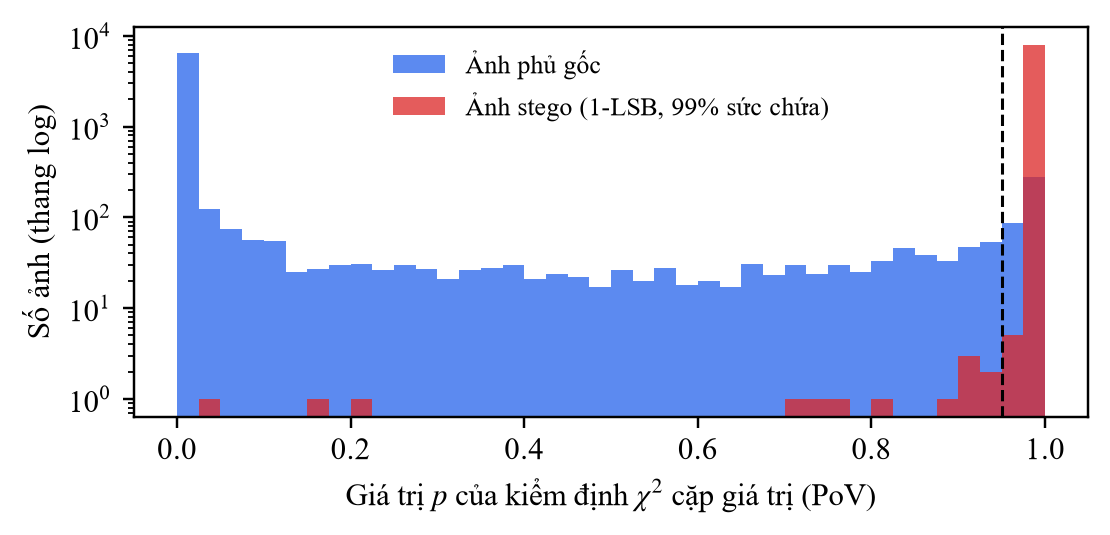
\includegraphics[width=0.82\linewidth]{chi2_steganalysis}
\caption{Phân bố giá trị $p$ của kiểm định $\chi^2$ cặp giá trị trên 8000 ảnh phủ và 8000 ảnh stego
(đường đứt: ngưỡng $p = 0.95$)}
\label{fig:chi2}
\end{figure}

\subsection{Tổng hợp đánh giá và đề xuất cải tiến}

\bang{tab:improve} tổng hợp các hạn chế đã được kiểm chứng bằng thực nghiệm và hướng khắc phục tương
ứng.

\begin{table}[H]
\centering
\caption{Các hạn chế đã kiểm chứng và đề xuất cải tiến}
\label{tab:improve}
\small
\begin{tabularx}{\linewidth}{@{}P{4.5cm}L@{}}
\toprule
\thead{Hạn chế} & \thead{Đề xuất khắc phục}\\
\midrule
Chaotic dùng lại dòng khóa; tham số công khai; không khuếch tán
  & Dẫn xuất dòng khóa từ khóa bí mật và một nonce ngẫu nhiên lưu trong header; tốt hơn là dùng mã dòng chuẩn như ChaCha20\\
IV cố định cho CBC: hai ảnh giống phần đầu cho bản mã giống phần đầu
  & Sinh IV ngẫu nhiên cho mỗi lần mã hóa và lưu vào header (IV không cần bí mật)\\
Không xác thực bản mã; CRC không chống sửa đổi có chủ đích
  & Dùng mã hóa có xác thực AES-GCM \cite{sp80038d} (hoặc ChaCha20-Poly1305) và đưa header vào dữ liệu liên kết (AAD) để mọi sửa đổi đều bị phát hiện\\
Khóa dẫn xuất từ seed công khai / SHA-256 của mật khẩu
  & Dùng hàm dẫn xuất khóa chậm có muối như Argon2 \cite{rfc9106} hoặc PBKDF2\\
3DES đã bị NIST loại bỏ, khối 64 bit dễ bị tấn công va chạm
  & Chỉ giữ 3DES để so sánh; dùng AES cho ứng dụng thực tế\\
LSB thay thế dễ bị kiểm định $\chi^2$ phát hiện
  & Dùng LSB matching ($\pm1$) \cite{mielikainen2006}, hoán vị vị trí nhúng bằng khóa, giảm tỷ lệ tải tin hoặc dùng giấu tin thích nghi \cite{holub2014}\\
Giấu tin không bền trước nén và nhiễu
  & Nếu cần độ bền: kết hợp mã sửa lỗi và nhúng trong miền biến đổi (DCT/DWT), chấp nhận giảm dung lượng\\
\bottomrule
\end{tabularx}
\end{table}


% =====================================================================
\chapter{Kết luận}
\label{chap:ketluan}
% =====================================================================

\section{Kết quả đạt được}

Đề tài đã nghiên cứu và tái hiện đầy đủ bài báo ``\BaiBaoGoc'' \cite{raut2026hybrid} từ MATLAB sang
Python. Các kết quả chính gồm:
\begin{itemize}
  \item \textbf{Về lý thuyết}: hệ thống hóa các kiến thức nền tảng của đề tài, gồm mã khối 3DES và
        AES ở chế độ CBC, đệm PKCS\#7, hệ hỗn loạn Logistic, mã dòng XOR, giấu tin LSB đa bit, và các
        tiêu chí đánh giá (MSE, PSNR, SSIM, NPCR, UACI, entropy, hệ số tương quan). Từ đó em rút ra
        công thức sai số kỳ vọng $(L^2-1)/6$ của phép nhúng $k$-LSB, giải thích được vì sao bài báo
        đạt $\mathrm{MSE} \approx 0.5$ và PSNR $\approx \SI{51.15}{dB}$.
  \item \textbf{Về cài đặt}: xây dựng thư viện lõi gồm ba thuật toán mã hóa theo mẫu Strategy, lớp
        giấu tin LSB 1--3 bit vectơ hóa hoàn toàn bằng NumPy, header 16 byte tự mô tả cho phép bên
        nhận giải mã chỉ từ ảnh stego và khóa, và bộ độ đo đánh giá kép. Hệ thống có 347 ca kiểm thử
        tự động, tất cả đều đạt.
  \item \textbf{Về tái hiện}: xác định và giải quyết nhất quán mười điểm mù kỹ thuật của bài báo.
        Trên toàn bộ 8000 ảnh Linnaeus 5 (\num{24000} lượt chạy), \textbf{100\%} ảnh bí mật được khôi
        phục chính xác từng bit. MSE ($0.4956$), PSNR (\SI{51.18}{dB}) và NPCR ($\approx 99.6\%$) khớp
        sát Bảng~2; thứ tự tốc độ Chaotic $<$ AES $<$ 3DES được giữ nguyên. Thời gian 3DES trên ảnh
        $246\times300$ (\SI{3588}{\micro s}) gần như trùng số liệu của bài báo (\SI{3552}{\micro s}).
  \item \textbf{Về phân tích}: giải thích được các con số ``bất thường'' trong Bảng~2. UACI thấp hơn
        $33.46\%$ là do phân bố mức xám của ảnh bí mật (giá trị kỳ vọng tính được là $30.41\%$);
        entropy $\approx 7.05$ thực chất là entropy của ảnh stego, trong khi entropy bản mã đạt
        $7.993$.
  \item \textbf{Về đánh giá an toàn mở rộng}: chỉ ra bằng thực nghiệm các hạn chế mà bài báo chưa
        nêu. Lớp Chaotic + PRNG bị phá hoàn toàn bởi tấn công biết bản rõ và không có tính khuếch tán
        (đổi một điểm ảnh chỉ đổi một byte bản mã). CBC với IV cố định chỉ khuếch tán về phía sau.
        Giấu tin LSB thay thế bị kiểm định $\chi^2$ phát hiện ở $99.84\%$ ảnh stego và bị phá hủy bởi
        nén JPEG hay nhiễu nhẹ.
  \item \textbf{Về sản phẩm}: xây dựng ứng dụng desktop bốn tab chạy ngoại tuyến, gồm mã hóa và giấu
        tin, giải mã kèm phòng thí nghiệm tấn công, so sánh ba thuật toán, và bảng điều khiển kết quả
        8000 ảnh. Ứng dụng được đóng gói thành tệp \code{.exe} chạy độc lập trên Windows.
\end{itemize}

Về câu hỏi nên chọn thuật toán nào, kết quả của báo cáo cho thấy chất lượng ảnh stego \emph{không
phụ thuộc} thuật toán mã hóa, chỉ phụ thuộc số bit nhúng. Trong ba lựa chọn, \textbf{AES-128} là
phương án cân bằng nhất: nhanh nhờ AES-NI, là chuẩn được công nhận rộng rãi, và chống được tấn công
biết bản rõ. Phương án Chaotic + PRNG của bài báo chỉ nhanh hơn khi mặt nạ được tính sẵn, và không đủ
an toàn cho ứng dụng thực tế ở dạng hiện tại.

\section{Hạn chế}

\begin{itemize}
  \item Do bài báo không công bố mã nguồn, khóa và nhiều chi tiết cài đặt, bản tái hiện chỉ có thể
        bám sát ở mức các đại lượng có thể suy luận được. Một số chênh lệch nhỏ (SSIM, entropy ảnh
        stego) chưa xác định được nguyên nhân chính xác.
  \item Thời gian mã hóa được đo trên một máy tính cụ thể (Intel Core i3-1005G1) bằng Python, nên chỉ
        có ý nghĩa so sánh tương đối với MATLAB.
  \item Các cải tiến đề xuất ở \bang{tab:improve} mới dừng ở mức phân tích, chưa được cài đặt và đánh
        giá đầy đủ trong khuôn khổ đề tài.
  \item Phần đánh giá phân tích giấu tin mới dùng kiểm định $\chi^2$; chưa thử các phương pháp mạnh
        hơn như phân tích RS \cite{fridrich2001} hay các bộ phân loại học sâu.
\end{itemize}

\section{Hướng phát triển}

\begin{itemize}
  \item \textbf{Nâng cấp lớp mật mã}: thay CBC bằng mã hóa có xác thực AES-GCM \cite{sp80038d} với
        nonce ngẫu nhiên cho mỗi ảnh, đưa header vào dữ liệu liên kết để phát hiện mọi chỉnh sửa; dẫn
        xuất khóa từ mật khẩu bằng Argon2 \cite{rfc9106}.
  \item \textbf{Cải tiến lớp hỗn loạn}: thiết kế lại theo các yêu cầu của Alvarez và Li
        \cite{alvarez2006}, gồm khóa bí mật đủ dài, dòng khóa phụ thuộc nonce và có vòng khuếch tán
        trên toàn ảnh; sau đó đánh giá lại bằng phân tích vi sai đúng định nghĩa.
  \item \textbf{Cải tiến lớp giấu tin}: thử nghiệm LSB matching \cite{mielikainen2006}, hoán vị vị
        trí nhúng bằng khóa, giấu tin thích nghi theo độ phức tạp vùng ảnh \cite{holub2014}; đánh giá
        bằng phân tích RS và các bộ phát hiện dựa trên học máy.
  \item \textbf{Tăng độ bền vững}: kết hợp mã sửa lỗi và nhúng trong miền DCT/DWT để thông điệp sống
        sót qua nén JPEG.
  \item \textbf{Mở rộng ứng dụng}: hỗ trợ ảnh bí mật màu, video và âm thanh như hướng phát triển mà
        bài báo gốc đề xuất.
\end{itemize}


% ------------------------------------------------------------ tài liệu tham khảo
\bibliographystyle{unsrtnat}
\bibliography{references}

% ------------------------------------------------------------ phụ lục
\appendix
% =====================================================================
\chapter{Hướng dẫn cài đặt và sử dụng chương trình}
\label{app:huongdan}
% =====================================================================

\section{Cài đặt môi trường}

Chương trình chạy trên Windows với Python 3.12. Từ thư mục \code{SOURCES}, tạo môi trường ảo và cài
các thư viện cần thiết:

\begin{lstlisting}[style=plain]
py -3.12 -m venv .venv
.\.venv\Scripts\python.exe -m pip install -r requirements.txt
\end{lstlisting}

Bộ dữ liệu Linnaeus 5 được đặt trong thư mục \path{SOURCES/data/linnaeus5/}, gồm hai thư mục con
\code{train} và \code{test}, mỗi thư mục chứa năm lớp \code{berry}, \code{bird}, \code{dog},
\code{flower}, \code{other}. Cặp ảnh mẫu \code{cover.jpg} và \code{secret.png} nằm trong
\path{SOURCES/data/sample/}.

\section{Chạy kiểm thử và các kịch bản thực nghiệm}

\begin{lstlisting}[style=plain]
# 347 ca kiem thu tu dong
.\.venv\Scripts\pytest.exe -q
# Kich ban A (Hinh 4-5): ket qua trong results/single/
.\.venv\Scripts\python.exe -m scripts.run_single
# Kich ban B (Bang 2): ket qua trong results/*.csv
.\.venv\Scripts\python.exe -m scripts.run_benchmark --secret-size 156 156 --cache-chaotic-mask
\end{lstlisting}

Các tùy chọn dòng lệnh chính:
\begin{itemize}
  \item \code{--secret-size H W}: thay đổi kích thước ảnh bí mật (mặc định giữ $246\times300$);
  \item \code{--cache-chaotic-mask}: tính sẵn mặt nạ Chaotic, chỉ đo thời gian phép XOR;
  \item \code{--vary-key-per-image}: dùng khóa khác nhau cho mỗi ảnh trong benchmark;
  \item \code{--limit N}: chỉ chạy $N$ ảnh đầu tiên (chạy thử nhanh, chỉ \code{run\_benchmark});
  \item \code{--cover} (chỉ \code{run\_single}), \code{--secret}, \code{--config}: chỉ định ảnh phủ,
        ảnh bí mật, tệp cấu hình.
\end{itemize}

\section{Ứng dụng desktop}

\begin{lstlisting}[style=plain]
# chay giao dien
.\.venv\Scripts\python.exe app.py
# kiem tra khoi dong (tu dong dong cua so)
.\.venv\Scripts\python.exe app.py --smoke
# dong goi thanh dist\CT204_CryptoStego\
.\.venv\Scripts\pyinstaller.exe packaging\ct204_app.spec
\end{lstlisting}

Bản đóng gói chỉ cần giải nén thư mục \code{CT204\_CryptoStego} và chạy
\code{CT204\_CryptoStego.exe}, không cần cài Python. Ảnh stego luôn được lưu ở định dạng PNG; hệ thống
từ chối lưu JPEG vì nén mất dữ liệu sẽ phá hủy các bit LSB.

\section{Tái tạo hình ảnh và số liệu trong báo cáo}

Các hình và số liệu bổ sung trong Chương~\ref{chap:vandung} được sinh bởi các script trong thư mục
\path{Reports/My_reports/Latex/tools}. Chúng chạy bằng môi trường ảo của dự án và không sửa đổi mã
nguồn lõi:

\begin{lstlisting}[style=plain]
cd SOURCES
.\.venv\Scripts\python.exe ..\Reports\My_reports\Latex\tools\make_figures.py
.\.venv\Scripts\python.exe ..\Reports\My_reports\Latex\tools\make_theory_figures.py
.\.venv\Scripts\python.exe ..\Reports\My_reports\Latex\tools\run_experiments.py
\end{lstlisting}


\end{document}
